% 00_MAIN_ProposalTA.tex
%
% Master file for Final Project Proposal Template Structure.
%
% Copyright 2025 by Philip Tobianto Daely.
% This file's structural code is protected under copyright and is licensed
% under the terms of the LaTeX Project Public License (LPPL).
%
%-----------------------------------------------------------------------

\documentclass[12pt]{report}
\usepackage{booktabs}
\usepackage{array}
\usepackage{tus-style} % style file, berisi library yg dibutuhkan dan setting tampilan

% berikan library tambahan di bawah ini
\usepackage{algpseudocode} % environment algoritma
\usepackage[document]{ragged2e}
\usepackage{tikz}
\usetikzlibrary{shapes.geometric, arrows.meta, positioning}

\tikzset{
    process/.style={rectangle, minimum width=3cm, minimum height=1cm, text centered, draw=black, fill=blue!15},
    decision/.style={diamond, aspect=2, minimum width=3cm, minimum height=1cm, text centered, draw=black, fill=green!20},
    startstop/.style={rectangle, rounded corners, minimum width=3cm, minimum height=1cm, text centered, draw=black, fill=red!30},
    arrow/.style={thick, ->, >=Stealth}
}
%==============================================================
\judulbhsindonesia{Integrasi Reinforcement Learning dalam Automated Web Penetration Testing: Studi Kasus OWASP Juice Shop}  % judul bhs indonesia, huruf kapital
\judulbhsinggris{Integrating Reinforcement Learning in Automated Web Penetration Testing: A Case Study on OWASP Juice Shop} % judul bhs inggris, huruf kapital
\prodi{Teknologi Informasi} % prodi mhs, huruf kapital untuk huruf awal di tiap kata saja
\matakuliah{Penulisan Proposal (CBK4AAA2)} % nama MK yang mengadakan seminar proposal
\tahuncover{2026} % tahun di mana periode revisi proposal berakhir

\namamahasiswa{Kevin Imanuel Setiawan} % nama mahasiswa
\nimmahasiswa{1202230003} % NIM mahasiswa

% isi tanggal di mana revisi/versi final Proposal TA disetujui Kaprodi
\tanggal{28} % tanggal lembar pengesahan di-ttd
\bulan{April} % bulan lembar pengesahan di-ttd
\tahun{2026} % tahun lembar pengesahan di-ttd

\namakaprodi{Muhammad Adib Kamali, S.T., M.Eng.} % nama dan gelar kaprodi
\nipkaprodi{22970007} % NIP kaprodi
\namapembimbingsatu{Philip Tobianto Daely, S.T., M.Eng., Ph.D.} % nama dan gelar pembimbing 1
\nippembimbingsatu{19940002} % NIP pembimbing 1
\namapembimbingdua{Muhammad Adib Kamali, S.T., M.Eng.} % nama dan gelar pembimbing 2
\nippembimbingdua{22970007} % NIP pembimbing 2
%==============================================================

\begin{document}
%==============================================================
\pagestyle{empty}
\begin{titlepage}
\centering

\LARGE
\judulcover{\TheJudulIndonesia}

\vspace{0.5cm}

\judulcover{\textit{\TheJudulInggris}}

\vspace{1cm}

\normalsize
Proposal~Tugas~Akhir \\
Mata~Kuliah~\TheMataKuliah

\vspace{1cm}

\large
Disusun oleh: \\
\textbf{\TheNamaMahasiswa} \\
\TheNIMMahasiswa

\vfill


\includegraphics[height=46.41mm]{gambar/telulogo.png}

\vfill



\vspace{1cm}

\tulisancoverbesar{PROGRAM~STUDI~SARJANA~\MakeUppercase{\TheProdi}}\\
\vspace{0.2cm}
\tulisancoverbesar{DIREKTORAT~KAMPUS~SURABAYA}\\
\vspace{0.2cm}
\tulisancoverbesar{UNIVERSITAS~TELKOM}\\
\vspace{0.2cm}
\tulisancoverbesar{SURABAYA}\\
\vspace{0.2cm}
\tulisancoverbesar{\TheTahunCover}


\end{titlepage}
\clearpage % halaman sampul/cover
% tidak perlu diedit, kecuali ingin mengubah tampilan

%==============================================================
% --- Pengaturan Halaman Lembar Pengesahan ---
\pagenumbering{roman} 
\setcounter{page}{2}
\pagestyle{plain}

% Menghilangkan spasi kosong berlebih di atas judul

\begin{center}
    \vspace{-0.5cm} % Menarik gambar ke atas agar tidak pindah ke halaman baru
    
    % Gunakan width dan height dengan keepaspectratio agar gambar pas otomatis
    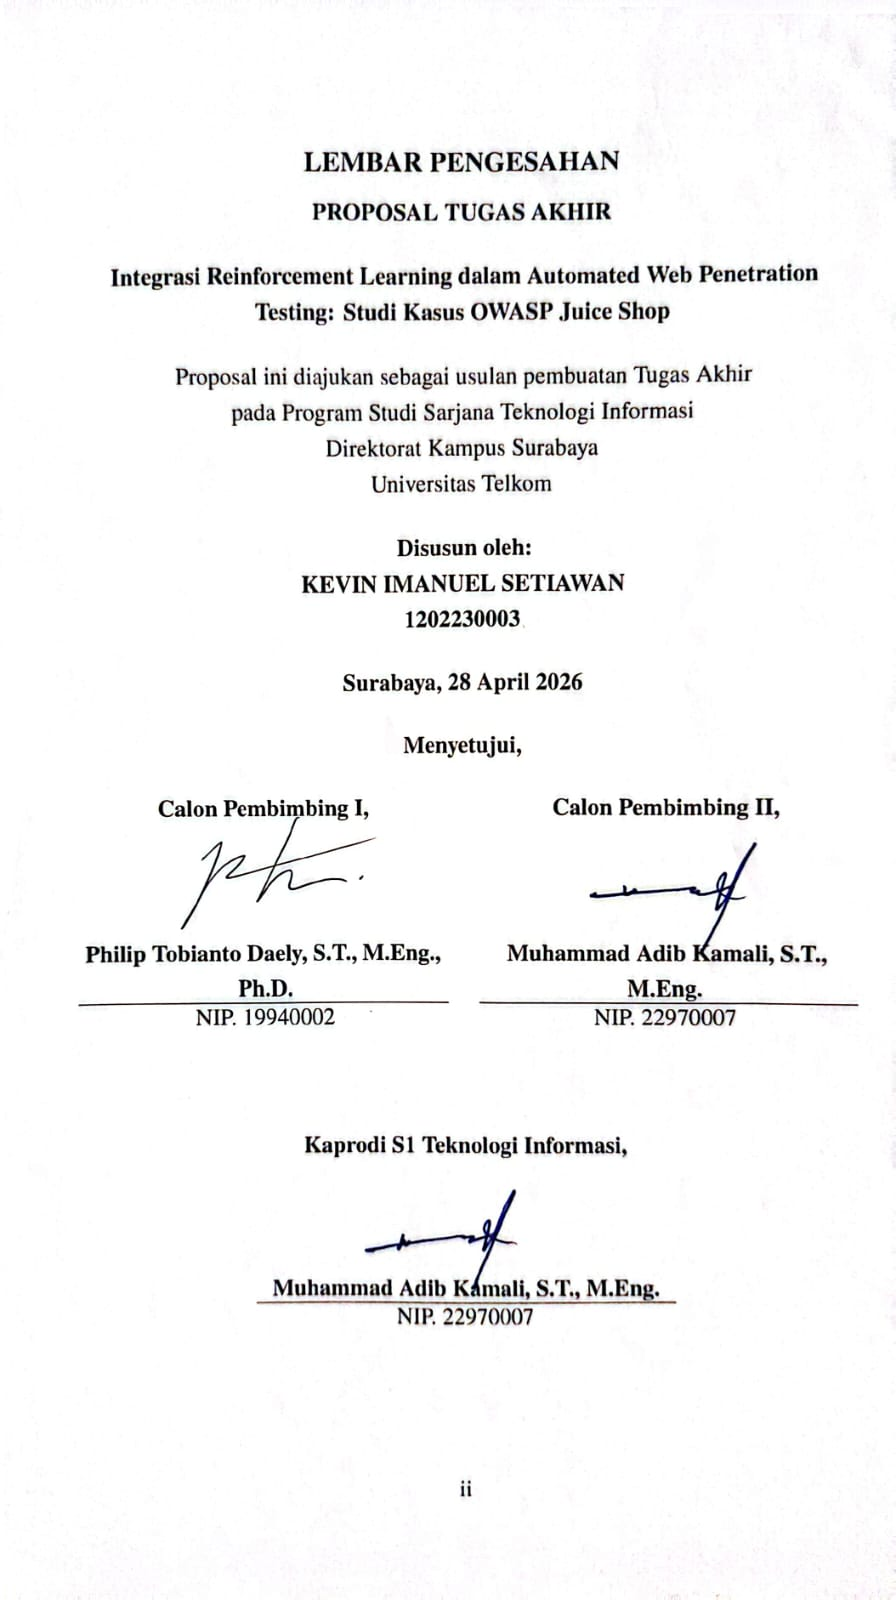
\includegraphics[width=0.95\textwidth, height=0.85\textheight, keepaspectratio]{gambar/pengesahan.jpeg}
\end{center} % lembar pengesahan
% tidak perlu diedit, kecuali ingin mengubah tampilan

%==============================================================
\tableofcontents % daftar isi
\addcontentsline{toc}{chapter}{Daftar Isi} 
% tidak perlu diedit
\clearpage

%==============================================================
\listoffigures % daftar gambar
\addcontentsline{toc}{chapter}{Daftar Gambar}
% jika tidak ada gambar, bagian ini bisa di-comment (nonaktif)
\clearpage

%==============================================================
\listoftables % daftar tabel
\addcontentsline{toc}{chapter}{Daftar Tabel}
% jika tidak ada tabel, bagian ini bisa di-comment (nonaktif)
\clearpage

%==============================================================
\chapter*{ABSTRAK}
\addcontentsline{toc}{chapter}{Abstrak} 

Perkembangan aplikasi web yang pesat meningkatkan risiko munculnya celah keamanan, seperti \textit{SQL Injection}, \textit{Cross-Site Scripting} (XSS), dan \textit{basic fuzzing}. Metode \textit{automated web penetration testing} konvensional yang masih berbasis aturan statis (\textit{rule-based}) memiliki keterbatasan dalam aspek adaptivitas dan efisiensi, terutama ketika menghadapi lingkungan web yang dinamis. Penelitian ini bertujuan untuk merancang dan mengimplementasikan metode \textit{Reinforcement Learning} dengan algoritma \textit{Q-Learning} dalam sistem \textit{automated web penetration testing}. Sistem dirancang agar agen dapat memilih strategi pengujian berdasarkan respons dari aplikasi target melalui mekanisme \textit{state}, \textit{action}, \textit{reward}, dan pembaruan \textit{Q-Table}. Pengujian dilakukan pada \textit{OWASP Juice Shop} dan dibandingkan dengan baseline menggunakan \textit{OWASP ZAP}. Evaluasi dilakukan berdasarkan jumlah kerentanan yang ditemukan, jumlah \textit{request}, waktu pengujian, \textit{precision}, dan \textit{cumulative reward}. Hasil yang diharapkan adalah sistem pengujian keamanan web otomatis yang lebih adaptif dan efisien dibandingkan dengan metode konvensional.

\textbf{Kata kunci:} \textit{penetration testing, reinforcement learning, Q-learning, web security, automated testing, OWASP Juice Shop.}
\clearpage


\chapter*{ABSTRACT}
\addcontentsline{toc}{chapter}{Abstract} 

The rapid development of web applications increases the risk of security vulnerabilities, such as SQL Injection, Cross-Site Scripting (XSS), and basic fuzzing. Conventional automated web penetration testing methods that rely on static rules are limited in adaptability and efficiency, especially in dynamic web environments. This study aims to design and implement a Reinforcement Learning method based on the Q-Learning algorithm for an automated web penetration testing system. The system is designed to enable the agent to select testing strategies based on responses from the target application via state, action, reward, and Q-Table updates. Testing is conducted on OWASP Juice Shop and compared with a baseline using OWASP ZAP. The evaluation is based on the number of detected vulnerabilities, the number of requests, testing time, precision, and cumulative reward. The expected result is an automated web security testing system that is more adaptive and efficient than conventional methods.

\textit{\textbf{Keywords:} penetration testing, reinforcement learning, Q-learning, web security, automated testing, OWASP Juice Shop.}
\clearpage % abstrak bhs indo dan eng. 
% Edit di file 03_abstrak_idn_eng.tex

%==============================================================
\pagenumbering{arabic} % set nomor halaman angka arab
\setcounter{page}{1}
% jangan di edit

%==============================================================
\chapter{Pendahuluan}

\section{Latar Belakang}

Perkembangan aplikasi berbasis web yang masif telah meningkatkan eksposur terhadap ancaman keamanan siber, menjadikan identifikasi kerentanan sebagai kebutuhan krusial dalam menjaga integritas sistem. Penetration testing merupakan pendekatan yang umum digunakan untuk mengevaluasi keamanan melalui simulasi serangan nyata. Namun, pendekatan konvensional terutama yang bersifat manual atau berbasis aturan statis masih menghadapi keterbatasan signifikan, seperti rendahnya efisiensi, tingginya ketergantungan pada keahlian spesialis, serta ketidakmampuan beradaptasi terhadap dinamika sistem yang kompleks dan terus berubah (\cite{zhang2023,kumar2024}).

Seiring dengan perkembangan machine learning, pendekatan berbasis pembelajaran adaptif mulai diadopsi untuk meningkatkan otomatisasi dalam penetration testing. Di antara berbagai metode, Reinforcement Learning (RL) menawarkan keunggulan dalam pengambilan keputusan berbasis pengalaman melalui interaksi langsung dengan lingkungan. RL memungkinkan agen untuk secara iteratif mengevaluasi dan mengoptimalkan strategi serangan berdasarkan umpan balik (reward), sehingga mampu mengeksplorasi ruang serangan secara lebih efektif dibandingkan dengan pendekatan deterministik (\cite{alavizadeh2024,nguyen2023}). Selain itu, penelitian terbaru menunjukkan bahwa pendekatan berbasis AI agent dan autonomous security systems memiliki potensi besar dalam meningkatkan efisiensi pengujian keamanan secara otomatis (\cite{li2025,chen2025}). Meskipun demikian, sebagian besar penelitian sebelumnya masih terbatas pada simulasi atau skenario umum, sehingga implementasi yang terukur pada aplikasi web nyata masih memerlukan eksplorasi lebih lanjut.

Berdasarkan kesenjangan tersebut, penelitian ini mengusulkan integrasi Reinforcement Learning sebagai mekanisme adaptive decision-making dalam automated web penetration testing. Studi ini menggunakan OWASP Juice Shop sebagai lingkungan pengujian untuk mengevaluasi kemampuan agen dalam mengidentifikasi kerentanan secara efisien dan adaptif. Dengan pendekatan ini, penelitian diharapkan dapat memberikan kontribusi dalam meningkatkan efektivitas strategi pengujian penetrasi dibandingkan dengan metode konvensional yang bersifat statis serta memberikan pendekatan yang lebih adaptif dalam menghadapi dinamika ancaman keamanan modern (\cite{singh2024}).

\section{Rumusan Masalah}
\begin{enumerate}
    \item Bagaimana merancang pendekatan \textit{Reinforcement Learning} dalam \textit{automated web penetration testing} untuk mengatasi keterbatasan metode pengujian konvensional yang masih bersifat statis, kurang adaptif, dan belum mempertimbangkan respons aplikasi web dalam pemilihan strategi pengujian kerentanan?
    
    \item Bagaimana merancang, mengimplementasikan, dan mengevaluasi metode \textit{Reinforcement Learning} dengan pendekatan Q-Learning dalam \textit{automated web penetration testing}, termasuk penentuan komponen \textit{state}, \textit{action}, \textit{reward}, pengaturan \textit{hyperparameter}, serta pengukuran kinerja berdasarkan waktu pengujian, jumlah \textit{request}, tingkat keberhasilan identifikasi kerentanan, dan \textit{cumulative reward}?
\end{enumerate}

\section{Tujuan Penelitian}
\begin{enumerate}
    \item Merancang sistem automated web penetration testing berbasis Reinforcement Learning (menggunakan algoritma Q-Learning) yang mampu mengadaptasi strategi pengujian kerentanan secara dinamis dengan mempertimbangkan respons balik dari web target guna mengatasi sifat statis pengujian konvensional.
    
    \item Merancang, mengimplementasikan, dan mengevaluasi metode \textit{Reinforcement Learning} dengan pendekatan Q-Learning dalam \textit{automated web penetration testing} melalui penentuan komponen \textit{state}, \textit{action}, \textit{reward}, pengaturan \textit{hyperparameter}, serta pengukuran kinerja berdasarkan waktu pengujian, jumlah \textit{request}, tingkat keberhasilan identifikasi kerentanan, dan \textit{cumulative reward}.
\end{enumerate}

\section{Manfaat Penelitian}

Penelitian ini diharapkan dapat memberikan manfaat dalam pengembangan ilmu pengetahuan di bidang keamanan siber dan kecerdasan buatan, khususnya terkait penerapan \textit{Reinforcement Learning} dalam proses \textit{automated web penetration testing}. Melalui penelitian ini, permasalahan pada metode pengujian konvensional yang kurang adaptif dan kurang efisien dapat dijelaskan secara lebih terarah, sehingga menjadi dasar dalam pengembangan pendekatan pengujian keamanan yang lebih mampu menyesuaikan strategi berdasarkan kondisi lingkungan pengujian.

Selain itu, penelitian ini diharapkan dapat memberikan manfaat praktis berupa rancangan dan implementasi metode Q-Learning untuk membantu proses identifikasi kerentanan pada aplikasi web secara lebih sistematis dan terukur. Hasil evaluasi berdasarkan waktu pengujian, jumlah \textit{request}, tingkat keberhasilan identifikasi kerentanan, dan \textit{cumulative reward} dapat digunakan sebagai dasar untuk menilai apakah pendekatan \textit{Reinforcement Learning} mampu memberikan peningkatan dibandingkan metode pengujian konvensional. Penelitian ini juga dapat menjadi referensi bagi penelitian selanjutnya yang ingin mengembangkan sistem pengujian keamanan otomatis dengan pendekatan pembelajaran adaptif.


\section{Batasan Penelitian}

Untuk menjaga fokus dan ruang lingkup penelitian, ditetapkan beberapa batasan sebagai berikut:

\begin{enumerate}
    \item Target pengujian terbatas pada aplikasi web OWASP Juice Shop sebagai studi kasus.
    \item Jenis serangan yang diuji meliputi SQL Injection, Cross-Site Scripting (XSS), dan basic fuzzing.
    \item Metode yang digunakan adalah Reinforcement Learning dengan pendekatan Q-Learning.
    \item Penelitian difokuskan pada pengujian keamanan aplikasi web dan tidak mencakup aspek keamanan jaringan atau sistem lainnya.
    \item Evaluasi sistem dilakukan berdasarkan metrik jumlah kerentanan yang ditemukan, waktu pengujian, jumlah request, dan cumulative reward. 
\end{enumerate}

\section{Sistematika Penulisan}

Sistematika penulisan dalam laporan penelitian ini disusun untuk memberikan gambaran alur pembahasan yang terstruktur. Adapun uraian singkat dari setiap bab adalah sebagai berikut:

\begin{enumerate}
    \item \textbf{Bab 1 - Pendahuluan} \\
    Bab ini menjelaskan latar belakang, rumusan masalah, tujuan, manfaat, batasan penelitian, serta sistematika penulisan sebagai panduan struktur keseluruhan laporan penelitian mengenai otomatisasi pengujian keamanan web.

    \item \textbf{Bab 2 - Tinjauan Pustaka} \\
    Bab ini membahas landasan konseptual dan teoritis yang mencakup definisi \textit{web penetration testing}, prinsip keamanan siber, teknologi \textit{Machine Learning} sebagai infrastruktur pendukung, serta \textit{Reinforcement Learning} sebagai mekanisme otomatisasi pengujian secara adaptif. Bab ini juga meninjau penelitian terdahulu sebagai pembanding dan penguat posisi penelitian.

    \item \textbf{Bab 3 - Metodologi dan Rancangan Sistem} \\
    Bab ini menjelaskan pendekatan penelitian dan tahapan pengembangan sistem menggunakan model \textit{prototyping}, spesifikasi alat dan bahan, perancangan arsitektur solusi yang memisahkan modul \textit{RL agent} dan \textit{pentest engine}, serta rancangan skenario serangan dan alur proses pembelajaran agen.
\end{enumerate} % ini file bab 1. 
% Edit di file 04_bab1.tex

%==============================================================
\chapter{TINJAUAN PUSTAKA}

\section{Kajian Teori}

\subsection{Web Penetration Testing}
\textit{Web penetration testing} merupakan metode pengujian keamanan aplikasi web dengan cara mensimulasikan serangan yang dilakukan oleh penyerang. Tujuan utama dari metode ini adalah untuk mengidentifikasi kerentanan yang dapat dimanfaatkan untuk mengakses sistem secara tidak sah.

Proses \textit{penetration testing} umumnya terdiri dari beberapa tahap, yaitu:
\begin{enumerate}
    \item \textbf{\textit{Information Gathering}}: Pengumpulan informasi target.
    \item \textbf{\textit{Vulnerability Scanning}}: Pemindaian celah keamanan.
    \item \textbf{\textit{Exploitation}}: Percobaan penetrasi pada celah yang ditemukan.
    \item \textbf{\textit{Reporting}}: Pelaporan hasil pengujian.
\end{enumerate}

Pendekatan ini sangat penting dalam menjaga keamanan sistem, namun memiliki keterbatasan jika dilakukan secara manual, seperti tidak efisien dan bergantung pada keahlian penguji. \textit{Penetration testing} tidak hanya berfungsi sebagai metode identifikasi kerentanan, tetapi juga sebagai mekanisme evaluasi terhadap efektivitas sistem keamanan yang telah diterapkan. Dalam praktiknya, proses ini meniru pola serangan yang dilakukan oleh penyerang nyata sehingga mampu memberikan gambaran yang lebih realistis terhadap potensi risiko yang dihadapi oleh sistem. Oleh karena itu, pendekatan ini menjadi salah satu metode yang paling banyak digunakan dalam pengujian keamanan aplikasi web (\cite{behl2017}).

\subsection{Vulnerability pada Aplikasi Web}

Kerentanan (\textit{vulnerability}) merupakan suatu kelemahan atau celah dalam desain, implementasi, operasi, maupun manajemen sistem yang dapat dieksploitasi oleh aktor ancaman (\textit{threat actor}) untuk melanggar kebijakan keamanan sistem tersebut. Pada arsitektur aplikasi web modern yang berbasis \textit{three-tier} (klien, server, dan database), kerentanan umumnya muncul akibat kegagalan dalam validasi input, sanitasi data yang tidak memadai, kesalahan konfigurasi keamanan (\textit{security misconfiguration}), serta kelemahan pada logika autentikasi dan otorisasi.

Untuk memberikan standardisasi dalam identifikasi risiko, \textit{Open Web Application Security Project} (OWASP) secara berkala merilis daftar risiko keamanan paling kritis. Berdasarkan metodologi pengujian keamanan aplikasi web, berikut adalah penjelasan rinci mengenai beberapa jenis kerentanan utama yang sering menjadi target eksploitasi:

\begin{enumerate}
    \item \textbf{\textit{SQL Injection} (SQLi)}
    
    \textit{SQL Injection} terjadi ketika data yang disuplai oleh pengguna (*user-supplied data*) langsung digabungkan ke dalam \textit{query} SQL tanpa melalui proses filtrasi atau menggunakan \textit{parameterized queries}. Akibatnya, interpreter database menginterpretasikan input tersebut sebagai perintah eksekusi, bukan sebagai data biasa. 
    
    
    
    Dampak dari serangan ini sangat fatal, meliputi kebocoran data sensitif (\textit{data exfiltration}), manipulasi atau penghapusan isi database (\textit{data tampering}), hingga pengambilalihan kontrol server database melalui fungsi \textit{stacked queries} atau \textit{command execution}.

    \item \textbf{\textit{Cross-Site Scripting} (XSS)}
    
    Kerentanan XSS terjadi ketika aplikasi web menyertakan data yang tidak terpercaya ke dalam halaman web yang dikirimkan ke \textit{browser} pengguna tanpa melakukan sanitasi atau \textit{output encoding} yang tepat. Hal ini memungkinkan penyerang untuk menyuntikkan \textit{malicious script} (umumnya berbasis JavaScript) yang akan dieksekusi oleh \textit{browser} korban dalam konteks sesi mereka. 
    
    
    
    Secara umum, XSS dibagi menjadi tiga kategori:
    \begin{itemize}
        \item \textbf{\textit{Stored XSS}}: \textit{Script} berbahaya disimpan secara permanen di server (misalnya pada database atau kolom komentar) dan dieksekusi setiap kali pengguna mengakses halaman tersebut.
        \item \textbf{\textit{Reflected XSS}}: \textit{Script} berbahaya dipantulkan dari \textit{request} HTTP (misalnya melalui parameter URL) langsung ke dalam \textit{response} tanpa disimpan.
        \item \textbf{\textit{DOM-based XSS}}: Eksekusi \textit{script} terjadi sepenuhnya di sisi klien akibat modifikasi \textit{Document Object Model} (DOM) oleh \textit{script} lokal yang tidak aman.
    \end{itemize}
    Dampak XSS meliputi pencurian token sesi (\textit{session hijacking}), pencurian kredensial melalui \textit{credential harvesting}, serta deface halaman web pada sisi klien.

    \item \textbf{\textit{Local File Inclusion} (LFI)}
    
    LFI adalah kerentanan yang terjadi ketika aplikasi web mengizinkan input dari pengguna untuk menentukan berkas yang akan dimuat atau dieksekusi secara lokal oleh server tanpa adanya validasi jalur (\textit{path validation}) yang ketat. Kerentanan ini sering ditemukan pada fungsi penanganan bahasa pemrograman web (seperti fungsi \texttt{include()}, \texttt{require()}, atau \texttt{file\_get\_contents()} pada PHP).
    
    Penyerang dapat menggunakan teknik \textit{directory traversal} (misalnya memasukkan urutan karakter \texttt{../../}) untuk membaca berkas sensitif di dalam sistem operasi server, seperti berkas konfigurasi aplikasi, \texttt{/etc/passwd} pada Linux, atau bahkan mencapai tahap \textit{Remote Code Execution} (RCE) melalui teknik \textit{log poisoning}.

    \item \textbf{\textit{Fuzzing} (Pengujian Kerentanan Otomatis)}
    
    Berbeda dengan tiga poin sebelumnya yang merujuk pada jenis celah keamanan, \textit{fuzzing} (atau \textit{fuzz testing}) merupakan teknik dan metodologi pengujian perangkat lunak yang digunakan untuk menemukan kerentanan tersembunyi secara otomatis. Proses ini dilakukan dengan cara memberikan input data yang tidak valid, tidak terduga, atau acak (\textit{malformed input}) dalam jumlah besar ke dalam titik masuk (\textit{entry point}) aplikasi web.
    
    Dalam konteks \textit{automated penetration testing}, \textit{fuzzing} digunakan untuk memicu perilaku anomali pada aplikasi, seperti \textit{error} internal server (HTTP 500), \textit{buffer overflow}, kebocoran informasi melalui pesan \textit{error}, atau \textit{unhandled exceptions}. Respons anomali inilah yang menjadi indikator kuat adanya celah keamanan yang dapat dieksploitasi lebih lanjut.
\end{enumerate}

Secara teoritis, pemahaman mendalam terhadap mekanisme dan karakteristik dari setiap kerentanan ini menjadi fondasi penting dalam merancang model keputusan (seperti pemetaan \textit{state} dan \textit{action} pada \textit{Reinforcement Learning}) untuk melakukan penetrasi atau pemindaian celah keamanan secara adaptif dan otomatis.

\subsection{Automated Penetration Testing}

\textit{Automated penetration testing} merupakan metode pengujian keamanan sistem yang dilakukan secara otomatis menggunakan perangkat lunak atau \textit{tools} tertentu untuk mengidentifikasi kerentanan pada aplikasi, jaringan, maupun sistem informasi (\cite{kumar2024}). Pendekatan ini dikembangkan untuk meningkatkan efisiensi proses \textit{penetration testing} dibandingkan metode manual yang cenderung membutuhkan waktu lebih lama dan sangat bergantung pada kemampuan seorang \textit{penetration tester}. Dengan adanya otomatisasi, proses pengujian dapat dilakukan secara lebih cepat, konsisten, dan mampu menangani cakupan sistem yang lebih luas.

Pada umumnya, \textit{automated penetration testing} bekerja dengan melakukan serangkaian tahapan secara otomatis, mulai dari proses \textit{information gathering}, \textit{vulnerability scanning}, analisis celah keamanan, hingga simulasi eksploitasi terhadap kerentanan yang ditemukan. Beberapa \textit{tools} yang umum digunakan dalam pendekatan ini antara lain \textit{Nmap} untuk pemetaan jaringan, \textit{Nikto} untuk pengujian keamanan web server, serta \textit{OWASP ZAP} dan \textit{Burp Suite} untuk pengujian aplikasi web. Penggunaan \textit{tools} tersebut memungkinkan proses pengujian dilakukan secara berulang dengan hasil yang lebih konsisten dibandingkan pengujian manual.

Selain meningkatkan efisiensi, \textit{automated penetration testing} juga membantu organisasi dalam melakukan pengujian keamanan secara berkala guna mendeteksi potensi kerentanan lebih dini. Pendekatan ini sangat bermanfaat pada lingkungan sistem modern yang memiliki kompleksitas tinggi dan perubahan konfigurasi yang cepat. Dengan pengujian otomatis, proses evaluasi keamanan dapat dilakukan secara kontinu sehingga membantu menjaga keamanan sistem secara lebih efektif.

Meskipun demikian, sebagian besar sistem \textit{automated penetration testing} saat ini masih menggunakan pendekatan \textit{rule-based} atau berbasis aturan yang telah ditentukan sebelumnya. Sistem hanya mampu menjalankan pola pengujian yang sudah diprogram dan cenderung kurang fleksibel dalam menghadapi kerentanan baru atau pola serangan yang dinamis. Ketika lingkungan sistem berubah atau muncul teknik serangan baru, sistem otomatis sering kali tidak dapat menyesuaikan strategi pengujiannya secara adaptif.

Keterbatasan tersebut menyebabkan proses pengujian keamanan belum sepenuhnya optimal, terutama dalam menghadapi aplikasi modern yang memiliki struktur dan perilaku yang kompleks. Oleh karena itu, diperlukan pendekatan yang lebih adaptif dan cerdas agar sistem \textit{automated penetration testing} mampu belajar dari lingkungan pengujian serta menentukan strategi pengujian yang lebih efektif secara otomatis. Salah satu pendekatan yang mulai banyak diteliti untuk mengatasi permasalahan tersebut adalah penerapan \textit{Reinforcement Learning} dalam proses \textit{penetration testing}.

\subsection{Machine Learning dalam Cybersecurity}

\textit{Machine Learning} merupakan cabang dari kecerdasan buatan (\textit{Artificial Intelligence}) yang memungkinkan sistem komputer mempelajari pola dari data dan membuat keputusan tanpa harus diprogram secara eksplisit (\cite{mitchell1997,singh2024}). Pendekatan ini bekerja dengan memanfaatkan data historis untuk membangun model yang dapat mengenali pola tertentu, melakukan prediksi, maupun mengambil keputusan secara otomatis. Seiring meningkatnya kompleksitas sistem digital dan jumlah ancaman siber, \textit{machine learning} menjadi salah satu teknologi yang banyak diterapkan dalam bidang keamanan siber.

Dalam konteks \textit{cybersecurity}, \textit{machine learning} dimanfaatkan untuk mendeteksi anomali perilaku sistem, mengidentifikasi aktivitas mencurigakan, mengklasifikasikan jenis serangan, serta menganalisis log keamanan dalam jumlah besar secara otomatis. Teknologi ini mampu membantu proses identifikasi ancaman yang sulit dideteksi menggunakan metode konvensional berbasis aturan (\textit{rule-based}). Dengan mempelajari pola lalu lintas jaringan dan aktivitas pengguna, sistem dapat mengenali indikasi serangan seperti \textit{malware}, \textit{phishing}, \textit{Distributed Denial of Service} (DDoS), maupun upaya eksploitasi celah keamanan lainnya.

Penerapan \textit{machine learning} dalam keamanan siber umumnya menggunakan beberapa pendekatan utama, yaitu \textit{supervised learning}, \textit{unsupervised learning}, dan \textit{reinforcement learning}. \textit{Supervised learning} digunakan ketika data pelatihan telah memiliki label sehingga sistem dapat mempelajari hubungan antara data dan kategori serangan tertentu. Sementara itu, \textit{unsupervised learning} digunakan untuk menemukan pola atau anomali pada data yang belum memiliki label. Adapun \textit{reinforcement learning} memungkinkan agen belajar melalui interaksi langsung dengan lingkungan berdasarkan mekanisme \textit{reward} dan \textit{punishment}.

Keunggulan utama \textit{machine learning} dalam \textit{cybersecurity} terletak pada kemampuannya dalam memproses data dalam skala besar dan melakukan adaptasi terhadap pola ancaman baru. Sistem dapat terus meningkatkan performanya seiring bertambahnya data yang dipelajari. Hal ini menjadikan \textit{machine learning} lebih fleksibel dibandingkan pendekatan tradisional yang hanya mengandalkan aturan statis.

Meskipun demikian, penerapan \textit{machine learning} dalam keamanan siber juga memiliki beberapa tantangan. Kualitas dan jumlah data pelatihan sangat memengaruhi performa model yang dihasilkan. Selain itu, model yang tidak dilatih dengan baik dapat menghasilkan \textit{false positive} atau \textit{false negative} yang berpotensi mengurangi efektivitas sistem keamanan. Kompleksitas proses pelatihan dan kebutuhan sumber daya komputasi yang tinggi juga menjadi salah satu tantangan dalam implementasinya.

Dengan berbagai kemampuan tersebut, \textit{machine learning} menjadi teknologi yang menjanjikan untuk mendukung pengembangan sistem keamanan siber yang lebih adaptif, termasuk dalam bidang \textit{automated penetration testing}. Integrasi \textit{machine learning}, khususnya \textit{reinforcement learning}, diharapkan mampu meningkatkan kemampuan sistem dalam menentukan strategi pengujian keamanan secara otomatis dan dinamis sesuai kondisi lingkungan pengujian.a

\subsection{Reinforcement Learning}
\textit{Reinforcement Learning} (RL) merupakan metode pembelajaran berbasis interaksi antara agen dan lingkungan (\cite{sutton2018}). Dalam metode ini, agen belajar memilih tindakan (\textit{action}) terbaik berdasarkan umpan balik yang diterima dari lingkungan dalam bentuk \textit{reward}. Proses pembelajaran dilakukan secara bertahap melalui percobaan berulang sehingga agen dapat menemukan strategi yang paling optimal.

Komponen utama dalam \textit{Reinforcement Learning} meliputi:
\begin{enumerate}
    \item \textbf{\textit{State}}: Representasi kondisi sistem saat ini.
    \item \textbf{\textit{Action}}: Tindakan yang diambil oleh agen.
    \item \textbf{\textit{Reward}}: Nilai positif atau negatif sebagai umpan balik dari lingkungan.
    \item \textbf{\textit{Agent \& Environment}}: Subjek yang belajar dan dunia tempat agen berinteraksi.
\end{enumerate}

Hubungan antara komponen-komponen tersebut dapat digambarkan dalam suatu siklus interaksi antara agen dan lingkungan, seperti ditunjukkan pada Gambar berikut.

\begin{figure}[H]
\centering
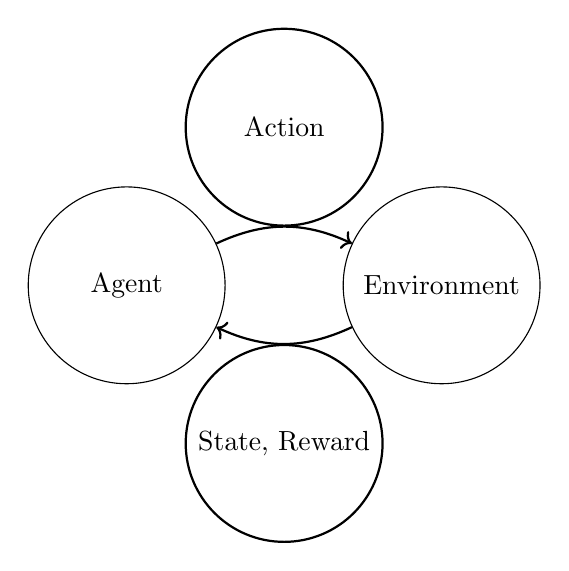
\begin{tikzpicture}[
    node distance=4cm,
    every node/.style={draw, circle, minimum size=2.5cm, align=center},
    arrow/.style={->, thick}
]
\node (agent) {Agent};
\node (env) [right of=agent] {Environment};

\draw[arrow] (agent) to[bend left=25] node[above] {Action} (env);
\draw[arrow] (env) to[bend left=25] node[below] {State, Reward} (agent);
\end{tikzpicture}
\caption{Konsep Reinforcement Learning}
\end{figure}

Gambar tersebut menunjukkan bahwa agen melakukan suatu tindakan terhadap lingkungan, kemudian lingkungan memberikan respons berupa \textit{state} baru dan \textit{reward}. Proses ini berlangsung secara terus-menerus sehingga agen dapat belajar dari pengalaman dan meningkatkan kualitas keputusan yang diambil.

Keunggulan utama \textit{Reinforcement Learning} dibandingkan metode \textit{machine learning} lainnya terletak pada kemampuannya dalam belajar melalui interaksi langsung dengan lingkungan, tanpa memerlukan dataset berlabel secara eksplisit.

\subsection{Reinforcement Learning dalam Penetration Testing}
Dalam konteks ini, RL digunakan untuk menentukan strategi pengujian secara adaptif. Agen akan memilih \textit{payload} atau tindakan tertentu, kemudian mengevaluasi hasilnya untuk meningkatkan strategi berikutnya.

Secara umum, proses penerapan \textit{Reinforcement Learning} dalam \textit{penetration testing} dapat digambarkan sebagai suatu alur interaksi antara agen, sistem target, dan mekanisme evaluasi, seperti ditunjukkan pada Gambar berikut.

\begin{figure}[H]
\centering
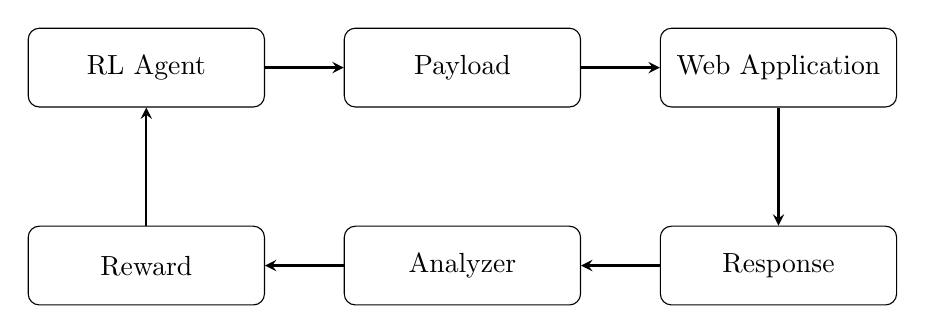
\begin{tikzpicture}[
    block/.style={
        draw, rectangle, rounded corners,
        minimum width=3cm, minimum height=1cm, align=center,
        fill=white
    },
    arrow/.style={->, >=stealth, thick}
]

\node[block] (agent) {RL Agent};
\node[block] (payload) [right=1cm of agent] {Payload};
\node[block] (web) [right=1cm of payload] {Web Application};

\node[block] (response) [below=1.5cm of web] {Response};
\node[block] (analyzer) [below=1.5cm of payload] {Analyzer};
\node[block] (reward) [below=1.5cm of agent] {Reward};

\draw[arrow] (agent) -- (payload);
\draw[arrow] (payload) -- (web);
\draw[arrow] (web) -- (response);
\draw[arrow] (response) -- (analyzer);
\draw[arrow] (analyzer) -- (reward);
\draw[arrow] (reward) -- (agent);

\end{tikzpicture}
\caption{Penerapan Reinforcement Learning dalam Penetration Testing}
\end{figure}

Gambar tersebut menunjukkan bahwa agen akan memilih \textit{payload} untuk dikirim ke aplikasi web. Selanjutnya, sistem akan memberikan respons yang kemudian dianalisis untuk menentukan apakah terdapat indikasi kerentanan. Hasil analisis ini digunakan untuk memberikan \textit{reward} kepada agen sebagai dasar dalam memperbaiki strategi pada langkah berikutnya.

Pendekatan ini memungkinkan eksplorasi \textit{attack path} yang lebih luas dan tidak terduga, pengambilan keputusan yang adaptif terhadap mekanisme proteksi server, serta peningkatan efisiensi pengujian melalui eliminasi tindakan yang tidak efektif.

\section{Penelitian Terkait}

\subsubsection{Literature Review}

\begin{table}[H]
\centering
\footnotesize
\renewcommand{\arraystretch}{1.2}
\setlength{\tabcolsep}{3pt}

\begin{tabularx}{\textwidth}{|c|p{3.2cm}|l|c|X|X|X|}
\hline
\textbf{No} & \textbf{Judul Penelitian} & \textbf{Peneliti} & \textbf{Tahun} & \textbf{Kelebihan} & \textbf{Kekurangan} & \textbf{Hasil} \\ \hline

1 & PentestGPT: Evaluating and Harnessing LLMs for Automated Pentesting & Deng et al. & 2023 & Otomatisasi berbasis AI modern & Tidak menggunakan RL & Efektivitas pentesting meningkat \\ \hline

2 & Large Language Models in Cybersecurity: Opportunities & Khoury et al. & 2023 & Analisis AI komprehensif & Masih bersifat konseptual & Potensi besar pada automation \\ \hline

3 & AutoPentest: Automated Penetration Testing Using AI Planning & Zhang et al. & 2023 & Pendekatan berbasis AI planning & Tidak adaptif seperti RL & Efisiensi pentesting meningkat \\ \hline

4 & Reinforcement Learning for Cybersecurity: A Survey & Nguyen et al. & 2023 & Fokus RL dalam security & Tidak spesifik web pentest & RL efektif untuk adaptive defense \\ \hline

5 & Deep Reinforcement Learning for Cyber Attack Detection & Alavizadeh et al. & 2024 & RL untuk decision-making & Fokus deteksi, bukan pentest & Akurasi keputusan meningkat \\ \hline

6 & AI-Driven Vulnerability Detection in Web Applications & Singh et al. & 2024 & Fokus pada kerentanan web & Tidak menggunakan RL & Peningkatan deteksi celah \\ \hline

7 & Automated Security Testing Using Machine Learning & Kumar et al. & 2024 & ML tingkatkan efisiensi testing & Tidak adaptif penuh & Mempercepat proses scanning \\ \hline

8 & Advances in Autonomous Cybersecurity Systems & Li et al. & 2025 & Sistem keamanan otonom berbasis AI & Masih bersifat umum & Menuju sistem security otomatis \\ \hline

9 & Intelligent Web Security Testing Using AI Agents & Chen et al. & 2025 & AI agent untuk web testing & Belum fokus pada RL & Agent tingkatkan efisiensi testing \\ \hline

\end{tabularx}
\caption{Ringkasan Penelitian Terdahulu (1--9)}
\end{table}

Kajian literatur dalam penelitian ini dilakukan untuk memahami perkembangan penelitian terkait \textit{automated penetration testing}, pemanfaatan \textit{machine learning} dalam keamanan siber, serta penerapan \textit{Reinforcement Learning} pada proses pengujian keamanan aplikasi web.

Literatur yang digunakan dalam penelitian ini dipilih berdasarkan keterkaitannya dengan tiga aspek utama. Pertama, penelitian yang membahas \textit{automated penetration testing} sebagai dasar perbandingan terhadap metode pengujian konvensional. Kedua, penelitian yang membahas pemanfaatan kecerdasan buatan atau \textit{machine learning} dalam mendukung proses deteksi dan pengujian kerentanan. Ketiga, penelitian yang membahas \textit{Reinforcement Learning} sebagai metode pengambilan keputusan adaptif pada lingkungan keamanan siber.

Berdasarkan hasil kajian literatur, diketahui bahwa sebagian besar pendekatan \textit{automated penetration testing} masih bersifat \textit{rule-based}, berbasis pemindaian statis, atau belum menggunakan mekanisme pembelajaran adaptif secara langsung pada aplikasi web. Oleh karena itu, penelitian ini memosisikan \textit{Reinforcement Learning} dengan algoritma \textit{Q-Learning} sebagai pendekatan yang digunakan untuk meningkatkan adaptivitas dan efisiensi dalam proses \textit{automated web penetration testing}.


\subsection{Analisis Penelitian Terdahulu}

Penelitian terdahulu memiliki peran penting sebagai dasar dalam memahami perkembangan pendekatan otomatisasi pengujian keamanan, khususnya pada bidang \textit{automated penetration testing}. Melalui kajian terhadap beberapa penelitian sebelumnya, dapat diketahui metode, kelebihan, keterbatasan, serta peluang pengembangan yang masih dapat diteliti lebih lanjut. Kajian ini juga digunakan untuk memperjelas posisi penelitian yang dilakukan, terutama dalam penerapan \textit{Reinforcement Learning} sebagai mekanisme pengambilan keputusan adaptif pada pengujian keamanan aplikasi web.

Berdasarkan Tabel 2.1, dapat disimpulkan bahwa pemanfaatan kecerdasan buatan dalam \textit{penetration testing} mengalami perkembangan yang signifikan, khususnya dalam penggunaan \textit{machine learning} dan AI berbasis \textit{agent}. Penelitian oleh Deng et al, menunjukkan bahwa \textit{large language model} mampu meningkatkan efektivitas \textit{penetration testing}, sementara Zhang et al. (\cite{zhang2023}) mengembangkan sistem \textit{automated pentesting} berbasis \textit{AI planning} yang meningkatkan efisiensi pengujian.

Selain itu, penelitian oleh Nguyen et al. (\cite{nguyen2023}) serta Alavizadeh et al. (\cite{alavizadeh2024}) menunjukkan bahwa \textit{reinforcement learning} memiliki potensi dalam pengambilan keputusan adaptif pada sistem keamanan siber. Pendekatan ini memungkinkan sistem untuk belajar dari interaksi dengan lingkungan sehingga mampu meningkatkan performa secara bertahap.

Namun demikian, sebagian besar penelitian masih memiliki keterbatasan, seperti tidak spesifik diterapkan pada aplikasi web, berfokus pada deteksi dibanding eksploitasi, atau belum mengintegrasikan \textit{reinforcement learning} sebagai mekanisme utama dalam \textit{automated penetration testing}. Oleh karena itu, penelitian ini berfokus pada integrasi \textit{reinforcement learning} untuk \textit{adaptive decision-making} dalam \textit{automated web penetration testing} pada lingkungan nyata, yaitu OWASP Juice Shop.

\section{Alur Penelitian}

\begin{figure}[H]
\centering
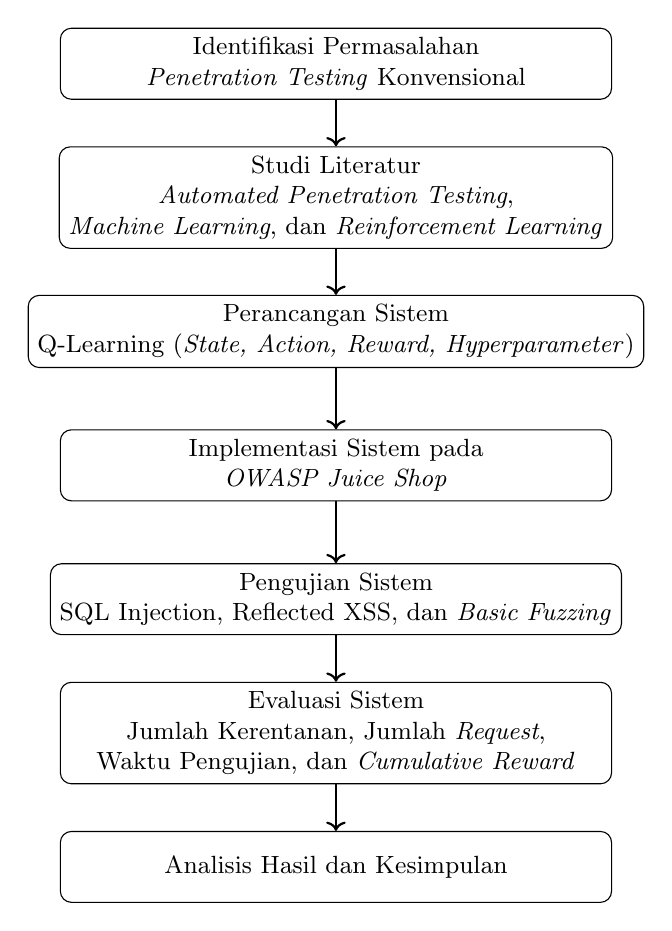
\begin{tikzpicture}[
    node distance=1.7cm,
    every node/.style={font=\small},
    process/.style={
        rectangle,
        draw=black,
        rounded corners,
        align=center,
        minimum width=7cm,
        minimum height=0.9cm
    },
    arrow/.style={
        ->,
        thick
    }
]

\node (start) [process] {Identifikasi Permasalahan \\ \textit{Penetration Testing} Konvensional};

\node (literature) [process, below of=start] {Studi Literatur \\ \textit{Automated Penetration Testing}, \\ \textit{Machine Learning}, dan \textit{Reinforcement Learning}};

\node (design) [process, below of=literature] {Perancangan Sistem \\ Q-Learning (\textit{State, Action, Reward, Hyperparameter})};

\node (implementation) [process, below of=design] {Implementasi Sistem pada \\ \textit{OWASP Juice Shop}};

\node (testing) [process, below of=implementation] {Pengujian Sistem \\ SQL Injection, Reflected XSS, dan \textit{Basic Fuzzing}};

\node (evaluation) [process, below of=testing] {Evaluasi Sistem \\ Jumlah Kerentanan, Jumlah \textit{Request}, \\ Waktu Pengujian, dan \textit{Cumulative Reward}};

\node (analysis) [process, below of=evaluation] {Analisis Hasil dan Kesimpulan};

\draw [arrow] (start) -- (literature);
\draw [arrow] (literature) -- (design);
\draw [arrow] (design) -- (implementation);
\draw [arrow] (implementation) -- (testing);
\draw [arrow] (testing) -- (evaluation);
\draw [arrow] (evaluation) -- (analysis);

\end{tikzpicture}
\caption{Alur Penelitian}
\label{fig:alur_penelitian}
\end{figure}

Alur penelitian ini dimulai dari adanya permasalahan pada proses \textit{penetration testing} konvensional yang masih memiliki beberapa keterbatasan. Pengujian secara manual atau berbasis aturan tetap cenderung membutuhkan waktu yang lebih lama, bergantung pada keahlian penguji, dan kurang mampu menyesuaikan diri terhadap kondisi sistem yang berubah.

Berdasarkan permasalahan tersebut, penelitian ini mengusulkan penggunaan \textit{Reinforcement Learning} sebagai pendekatan untuk membantu proses \textit{automated penetration testing}. Melalui pendekatan ini, sistem dirancang agar dapat belajar dari setiap percobaan pengujian yang dilakukan. Agen akan memilih aksi berupa payload tertentu, mengirimkannya ke aplikasi target, kemudian menerima respons dari sistem sebagai dasar untuk menentukan tindakan berikutnya.

Penelitian ini diterapkan pada aplikasi web \textit{OWASP Juice Shop} sebagai lingkungan pengujian. Sistem akan diuji untuk melihat kemampuannya dalam menemukan kerentanan seperti \textit{SQL Injection}, \textit{Reflected Cross-Site Scripting} (Reflected XSS), dan \textit{basic fuzzing}. Hasil pengujian kemudian dievaluasi berdasarkan beberapa metrik, yaitu jumlah kerentanan yang ditemukan, jumlah \textit{request}, waktu pengujian, dan nilai \textit{cumulative reward}.

Dengan alur tersebut, penelitian ini diharapkan dapat menunjukkan apakah pendekatan \textit{Reinforcement Learning} mampu meningkatkan efektivitas dan efisiensi proses \textit{penetration testing} dibandingkan dengan pendekatan konvensional. % ini file bab 2. 
% Edit di file 05_bab2.tex

%==============================================================
\chapter{METODOLOGI DAN RANCANGAN PENELITIAN}

\section{Metodologi Penelitian}
Penelitian ini menerapkan metode \textit{Prototyping} untuk memungkinkan pengembangan sistem secara bertahap dan iteratif. Pendekatan ini dipilih karena sesuai dengan karakteristik sistem \textit{Reinforcement Learning} yang memerlukan proses evaluasi dan perbaikan secara berulang untuk mencapai performa yang optimal.

Metode Prototyping dalam penelitian ini dilakukan melalui beberapa tahapan utama, yaitu identifikasi kebutuhan sistem, perancangan sistem awal, pembangunan prototipe, pengujian sistem, serta evaluasi dan perbaikan. Setiap tahap dilakukan secara berulang hingga sistem yang dikembangkan mampu mencapai tujuan yang diharapkan.

\begin{figure}[H]
\centering
\resizebox{0.95\textwidth}{!}{
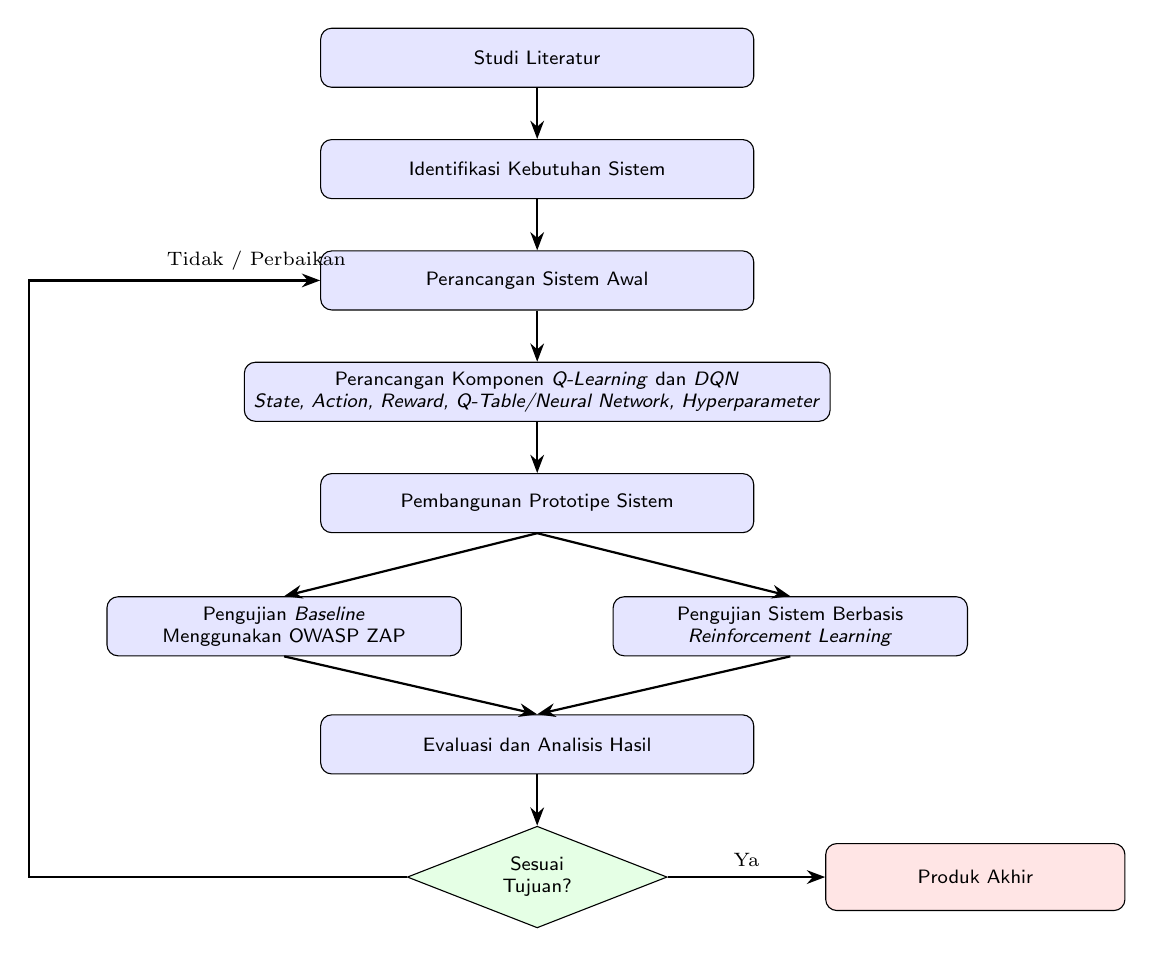
\begin{tikzpicture}[
    node distance=0.65cm and 0.8cm,
    auto,
    process/.style={
        draw, rectangle, rounded corners, 
        minimum width=5.5cm, minimum height=0.75cm, 
        align=center, fill=blue!10, font=\scriptsize\sffamily
    },
    process_split/.style={
        draw, rectangle, rounded corners, 
        minimum width=4.5cm, minimum height=0.75cm, 
        align=center, fill=blue!10, font=\scriptsize\sffamily
    },
    decision/.style={
        draw, diamond, aspect=2,
        minimum width=3.3cm, minimum height=0.85cm, 
        align=center, fill=green!10, font=\scriptsize\sffamily
    },
    startstop/.style={
        draw, rectangle, rounded corners, 
        minimum width=3.8cm, minimum height=0.85cm, 
        align=center, fill=red!10, font=\scriptsize\sffamily
    },
    arrow/.style={
        -Stealth, thick
    }
]

    % Alur Utama Atas (Gunakan koordinat atau placeholder jika bagian atas ingin dipastikan presisi)
    \node (n1) [process] {Studi Literatur};
    \node (n2) [process, below=of n1] {Identifikasi Kebutuhan Sistem};
    \node (n3) [process, below=of n2] {Perancangan Sistem Awal};
    \node (n4) [process, below=of n3] {Perancangan Komponen \textit{Q-Learning} dan \textit{DQN}\\
    \textit{State, Action, Reward, Q-Table/Neural Network, Hyperparameter}};
    \node (n5) [process, below=of n4] {Pembangunan Prototipe Sistem};

    % Alur Paralel (Bercabang ke Kiri dan Kanan)
    \node (n6) [process_split, below left=0.8cm and -1.8cm of n5] {Pengujian \textit{Baseline}\\Menggunakan OWASP ZAP};
    \node (n7) [process_split, below right=0.8cm and -1.8cm of n5] {Pengujian Sistem Berbasis\\\textit{Reinforcement Learning}};

    % Alur Penggabungan Bawah
    \node (n8) [process, below=2.3cm of n5] {Evaluasi dan Analisis Hasil};
    \node (n9) [decision, below=of n8] {Sesuai\\Tujuan?};
    \node (n10) [startstop, right=of n9, xshift=1.2cm] {Produk Akhir};

    % Menghubungkan Garis Panah
    \draw [arrow] (n1) -- (n2);
    \draw [arrow] (n2) -- (n3);
    \draw [arrow] (n3) -- (n4);
    \draw [arrow] (n4) -- (n5);
    
    % Panah dari Prototipe ke Cabang Pengujian
    \draw [arrow] (n5.south) -- (n6.north);
    \draw [arrow] (n5.south) -- (n7.north);
    
    % Panah dari Pengujian ke Evaluasi
    \draw [arrow] (n6.south) -- (n8.north);
    \draw [arrow] (n7.south) -- (n8.north);
    
    \draw [arrow] (n8) -- (n9);
    \draw [arrow] (n9) -- node [anchor=south, font=\scriptsize] {Ya} (n10);

   
    \draw [arrow] (n9.west) -- ++(-4.8,0) |- (n3.west) 
        node [pos=0.85, above, font=\scriptsize, xshift=0.3cm] {Tidak / Perbaikan};

\end{tikzpicture}
}
\caption{Alur Metodologi Penelitian}
\label{fig:alur_metodologi_penelitian}
\end{figure}

\section{Alat dan Bahan yang Digunakan}

\subsection{Perangkat Lunak}

\begin{table}[H]
\centering
\begin{tabular}{|c|l|p{8cm}|}
\hline
\textbf{No} & \textbf{Komponen} & \textbf{Keterangan} \\ \hline

1 & Bahasa Pemrograman & Python dengan library NumPy untuk perhitungan Q-Table dan Requests untuk komunikasi HTTP \\ \hline

2 & Metode RL & Q-Learning dan Deep Q-Network (DQN) sebagai algoritma pembelajaran agen \\ \hline

3 & Target Lingkungan & OWASP Juice Shop \\ \hline

4 & Tools Pendukung & OWASP ZAP digunakan sebagai baseline pengujian dan integrasi melalui API \\ \hline

5 & Editor Kode & Visual Studio Code \\ \hline

\end{tabular}
\caption{Perangkat Lunak yang Digunakan}
\end{table}

\subsection{Perangkat Keras}

\begin{table}[H]
\centering
\begin{tabular}{|c|l|p{8cm}|}
\hline
\textbf{No} & \textbf{Komponen} & \textbf{Spesifikasi} \\ \hline

1 & Laptop/PC & Perangkat utama yang digunakan untuk menjalankan proses pengembangan sistem, pengujian, dan analisis hasil \\ \hline

2 & RAM & Minimal 8 GB \\ \hline

3 & Prosesor & Minimal Intel i5 atau setara \\ \hline

\end{tabular}
\caption{Perangkat Keras yang Digunakan}
\end{table}

\section{Perancangan Sistem Awal / Arsitektur Solusi}

\subsection{Analisis Aktor}

Analisis aktor dilakukan untuk mengidentifikasi komponen-komponen yang terlibat dalam sistem \textit{automated penetration testing} berbasis \textit{Reinforcement Learning}. Setiap aktor memiliki peran dan tanggung jawab masing-masing dalam mendukung proses pengujian keamanan secara otomatis dan adaptif. Pada penelitian ini, terdapat tiga aktor utama, yaitu Administrator, \textit{RL Agent}, dan \textit{Environment} berupa aplikasi \textit{OWASP Juice Shop}.

Administrator berperan sebagai pihak yang melakukan konfigurasi awal sistem sebelum proses pengujian dijalankan. Tugas administrator meliputi penentuan parameter pelatihan seperti \textit{learning rate}, nilai \textit{epsilon}, jumlah episode, serta pengaturan skenario pengujian yang akan digunakan. Selain itu, administrator juga bertanggung jawab dalam memantau hasil pengujian, mengevaluasi performa agen, serta menganalisis kerentanan yang berhasil ditemukan selama proses \textit{penetration testing}. Peran administrator sangat penting untuk memastikan sistem berjalan sesuai tujuan penelitian.

\textit{RL Agent} merupakan komponen inti dalam sistem yang berfungsi sebagai agen pembelajar. Agen bertugas menentukan aksi atau strategi pengujian yang akan dilakukan berdasarkan kondisi lingkungan yang diamati. Dalam prosesnya, agen akan menerima informasi berupa \textit{state} dari lingkungan, kemudian memilih tindakan tertentu seperti mengirimkan \textit{payload}, melakukan eksplorasi endpoint, atau mencoba pola serangan tertentu. Setelah aksi dilakukan, agen akan menerima \textit{reward} sebagai umpan balik atas keberhasilan atau kegagalan tindakan tersebut. Melalui mekanisme ini, agen dapat mempelajari strategi pengujian yang paling optimal secara bertahap.

Sementara itu, \textit{environment} dalam penelitian ini direpresentasikan oleh aplikasi \textit{OWASP Juice Shop} yang berfungsi sebagai target pengujian keamanan. Aplikasi ini dipilih karena memiliki berbagai jenis kerentanan keamanan web yang sesuai untuk kebutuhan simulasi \textit{penetration testing}. \textit{Environment} akan memberikan respons terhadap setiap aksi yang dilakukan oleh agen, seperti respons HTTP, status keberhasilan eksploitasi, maupun perubahan kondisi sistem tertentu. Respons tersebut kemudian digunakan sebagai dasar bagi agen untuk menentukan langkah pengujian berikutnya.

Interaksi antara administrator, \textit{RL Agent}, dan \textit{environment} membentuk suatu siklus pembelajaran yang berkelanjutan. Administrator melakukan konfigurasi sistem, agen menjalankan proses pengujian dan pembelajaran, sedangkan \textit{environment} menyediakan umpan balik yang digunakan agen untuk meningkatkan performanya. Dengan adanya interaksi tersebut, sistem diharapkan mampu melakukan \textit{automated penetration testing} secara lebih adaptif dibandingkan pendekatan konvensional berbasis aturan.

\usetikzlibrary{positioning, fit, arrows.meta, backgrounds}

\subsection{Keterkaitan Rancangan Sistem dengan Permasalahan Penelitian}

Rancangan sistem dalam penelitian ini disusun untuk menjawab permasalahan utama yang telah dijelaskan pada Bab 1, yaitu keterbatasan metode \textit{automated web penetration testing} konvensional dalam aspek adaptivitas dan efisiensi. Pada metode konvensional, proses pengujian umumnya dilakukan berdasarkan aturan atau daftar \textit{payload} yang telah ditentukan sebelumnya. Pendekatan tersebut cenderung menjalankan banyak percobaan tanpa mempertimbangkan hasil dari pengujian sebelumnya, sehingga dapat menghasilkan jumlah \textit{request} yang besar dan proses pengujian yang kurang efisien.

Untuk menjawab permasalahan tersebut, sistem yang dirancang dalam penelitian ini menggunakan pendekatan \textit{Reinforcement Learning} dengan algoritma Q-Learning. Agen tidak hanya mengirimkan \textit{payload} secara berulang, tetapi juga mempelajari hasil dari setiap aksi berdasarkan respons aplikasi target. Respons tersebut digunakan untuk membentuk \textit{state} dan memberikan nilai \textit{reward}, sehingga agen dapat memperbarui Q-Table dan menentukan strategi pengujian yang lebih tepat pada iterasi berikutnya.

Dengan rancangan tersebut, aspek adaptivitas dijawab melalui kemampuan agen dalam memilih aksi berdasarkan pengalaman sebelumnya, sedangkan aspek efisiensi dijawab melalui pengukuran jumlah \textit{request}, waktu pengujian, dan tingkat keberhasilan identifikasi kerentanan. Oleh karena itu, rancangan sistem tidak hanya menjelaskan implementasi metode, tetapi juga menunjukkan bagaimana metode yang diusulkan digunakan untuk menjawab problem utama penelitian.

\subsection{Arsitektur Sistem}
Sistem yang dikembangkan dirancang agar agen \textit{Reinforcement Learning} dapat melakukan proses \textit{penetration testing} melalui alur yang terintegrasi dari pengumpulan informasi hingga pemindaian kerentanan. Arsitektur sistem ditunjukkan pada Gambar \ref{fig:arsitektur_baru}.

\begin{figure}[h!]
\centering
\resizebox{\textwidth}{!}{
\begin{tikzpicture}[
    node distance=0.7cm and 1.2cm,
    block/.style={draw, rectangle, rounded corners, minimum width=2.8cm, minimum height=0.8cm, text centered, font=\scriptsize\sffamily},
    tallblock/.style={draw, rectangle, rounded corners, minimum width=1.1cm, minimum height=5.5cm, text centered, font=\small\bfseries\sffamily},
    arrow/.style={-Stealth, thick}
]

    \node (agent) [tallblock] {\rotatebox{90}{RL Agent (Q-Learning)}};

    \node (f1) [block, right=of agent.north east, anchor=north west, xshift=0.8cm, yshift=-0.2cm] {Endpoint Mapping};
    \node (f2) [block, below=of f1] {HTTP Headers};
    \node (f3) [block, below=of f2] {Input Fields};
    \node (f4) [block, below=of f3] {Auth Mechanism};

    \node (info) [tallblock, right=of f2, xshift=0.8cm, yshift=-0.4cm] {\rotatebox{90}{Information Gathering}};

    \node (v1) [block, right=of info.north east, anchor=north west, xshift=0.8cm, yshift=-1cm] {SQL Injection};
    \node (v2) [block, below=of v1, yshift=-0.5cm] {XSS};
    \node (v3) [block, below=of v2, yshift=-0.5cm] {Basic Fuzzing};

    \node (scan) [tallblock, right=of v2, xshift=0.8cm] {\rotatebox{90}{Analyze and Scan}};

    \begin{scope}[on background layer]
        \node[draw, rectangle, rounded corners, fill=gray!5, inner sep=12pt, fit=(v1) (v3) (scan), label={[font=\small\bfseries, yshift=2pt]above:Vulnerability Assessment}] (va_box) {};
    \end{scope}

    \foreach \n in {f1, f2, f3, f4} {
        \draw [arrow] (agent.east |- \n.west) -- (\n.west);
    }

    \foreach \n in {f1, f2, f3, f4} {
        \draw [arrow] (\n.east) -- (info.west |- \n.east);
    }

    \foreach \n in {v1, v2, v3} {
        \draw [arrow] (info.east |- \n.west) -- (\n.west);
    }

    \foreach \n in {v1, v2, v3} {
        \draw [arrow] (\n.east) -- (scan.west |- \n.east);
    }

\end{tikzpicture}
}
\caption{Arsitektur Sistem Penetration Testing Berbasis Reinforcement Learning}
\label{fig:arsitektur_baru}
\end{figure}

Berdasarkan Gambar \ref{fig:arsitektur_baru}, proses dimulai dari \textit{RL Agent} yang menentukan aksi berupa strategi pengujian. Aksi tersebut dikirimkan ke \textit{Pentest Engine} untuk menghasilkan \textit{HTTP request} yang akan dikirimkan ke aplikasi target \textit{OWASP Juice Shop}. Respons yang diterima kemudian dianalisis oleh \textit{Response Analyzer} untuk menghasilkan \textit{state} baru serta \textit{reward}, yang selanjutnya digunakan untuk memperbarui strategi agen.

Untuk memberikan gambaran yang lebih implementatif, arsitektur sistem dikembangkan menjadi lebih rinci seperti ditunjukkan pada Gambar \ref{fig:arsitektur_detail}.

\begin{figure}[h!]
\centering
\resizebox{\textwidth}{!}{
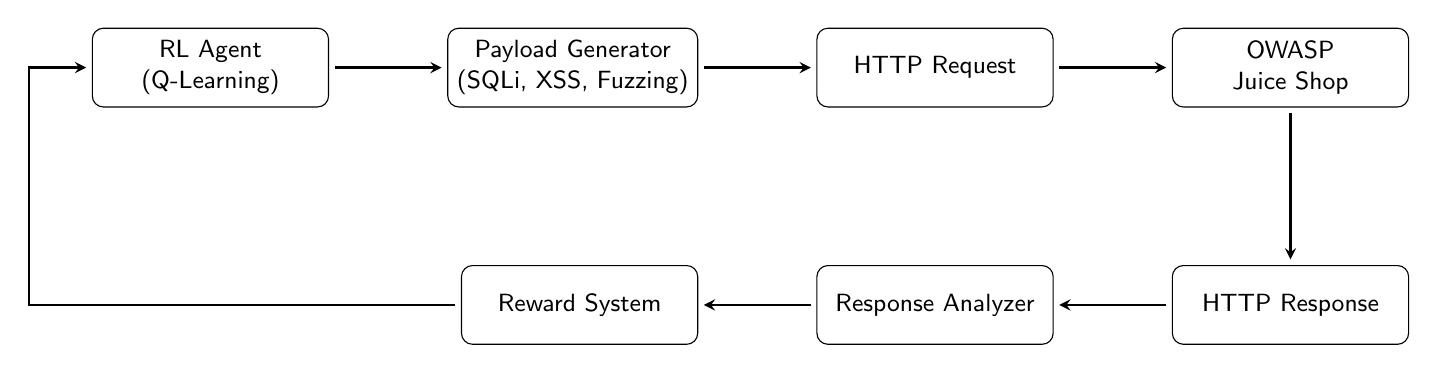
\begin{tikzpicture}[
    node distance=1.2cm and 1.5cm,
    block/.style={
        draw, 
        rectangle, 
        rounded corners=4pt, 
        minimum width=3cm, 
        minimum height=1cm, 
        align=center,
        fill=white,
        font=\small\sffamily
    },
    arrow/.style={
        ->, 
        >=stealth,
        thick, 
        shorten >=2pt, 
        shorten <=2pt
    }
]

\node[block] (agent) {RL Agent\\(Q-Learning)};
\node[block, right=of agent] (payload) {Payload Generator\\(SQLi, XSS, Fuzzing)};
\node[block, right=of payload] (request) {HTTP Request};
\node[block, right=of request] (target) {OWASP\\Juice Shop};

\node[block, below=2cm of target] (response) {HTTP Response};
\node[block, left=of response] (analyzer) {Response Analyzer};
\node[block, left=of analyzer] (reward) {Reward System};

\draw[arrow] (agent) -- (payload);
\draw[arrow] (payload) -- (request);
\draw[arrow] (request) -- (target);
\draw[arrow] (target) -- (response);
\draw[arrow] (response) -- (analyzer);
\draw[arrow] (analyzer) -- (reward);

\draw[arrow] (reward.west) -| ([xshift=-0.8cm]agent.west) -- (agent.west);

\end{tikzpicture}
}
\caption{Arsitektur Sistem Secara Detail}
\label{fig:arsitektur_detail}
\end{figure}

Pada Gambar \ref{fig:arsitektur_detail}, proses pengujian ditunjukkan secara lebih rinci. Agen \textit{Reinforcement Learning} memilih aksi berupa \textit{payload} tertentu, seperti \textit{SQL Injection}, \textit{Cross-Site Scripting} (XSS), atau \textit{fuzzing}. Payload tersebut dikirimkan melalui modul \textit{HTTP Request} menggunakan library Python ke aplikasi target. Respons yang diterima dianalisis untuk mengidentifikasi indikasi kerentanan, kemudian digunakan untuk menentukan nilai \textit{reward}. Nilai ini selanjutnya digunakan untuk memperbarui \textit{Q-Table}, sehingga agen dapat meningkatkan strategi pengujian secara adaptif pada iterasi berikutnya.

\subsection{Desain Komponen Reinforcement Learning}

Model \textit{Reinforcement Learning} dalam penelitian ini terdiri dari tiga komponen utama, yaitu \textit{state}, \textit{action}, dan \textit{reward}. \textit{State} (S) direpresentasikan sebagai kombinasi fitur dari respons sistem, seperti \textit{status code}, panjang respons, dan indikator error, yang kemudian diolah dalam bentuk representasi diskrit, misalnya tuple, agar dapat digunakan sebagai indeks dalam Q-Table.

\textit{Action} (A) merupakan aksi yang dilakukan oleh agen berupa pengiriman \textit{payload} ke aplikasi target. Payload yang digunakan dalam penelitian ini mencakup \textit{SQL Injection}, \textit{Reflected Cross-Site Scripting} (Reflected XSS), dan \textit{fuzzing}. Jenis XSS yang digunakan secara khusus adalah \textit{Reflected XSS}, bukan XSS secara umum, karena jenis serangan ini memberikan umpan balik yang lebih cepat dan terukur terhadap aksi yang dilakukan oleh agen. Pada Reflected XSS, payload dikirimkan melalui parameter URL atau input form, kemudian sistem menganalisis apakah payload tersebut muncul kembali pada respons HTTP. Karakteristik ini sesuai dengan kebutuhan Q-Learning karena keberhasilan atau kegagalan aksi dapat dievaluasi secara langsung melalui respons dari aplikasi target.

Sementara itu, \textit{reward} (R) diberikan sebagai umpan balik dari lingkungan. Nilai positif (+50) diberikan jika sistem berhasil menemukan indikasi kerentanan, misalnya ketika payload SQL Injection menghasilkan respons error tertentu atau ketika payload Reflected XSS berhasil muncul kembali pada isi respons HTTP tanpa proses sanitasi yang memadai. Sebaliknya, nilai negatif (-1) diberikan untuk setiap \textit{request} yang tidak menghasilkan temuan kerentanan. Selain itu, untuk mendukung proses pembelajaran, Q-Table direpresentasikan dalam bentuk struktur data seperti \textit{dictionary} dengan pasangan kunci \textit{(state, action)} dan nilai berupa estimasi $Q(s,a)$. Penentuan \textit{reward} ini bertujuan untuk mendorong agen menemukan kerentanan secara efisien dengan jumlah \textit{request} yang minimal \cite{nguyen2023}.

Agar komponen \textit{state}, \textit{action}, \textit{reward}, dan Q-Table dapat diimplementasikan secara sistematis, penelitian ini merancang struktur data utama yang digunakan dalam proses pengujian dan pembelajaran agen.

\subsection{Struktur Data Sistem}

Struktur data dalam penelitian ini dirancang untuk mendukung proses kerja sistem \textit{automated penetration testing} berbasis \textit{Reinforcement Learning}. Struktur data digunakan untuk menyimpan informasi yang diperoleh dari proses \textit{information gathering}, daftar \textit{payload} yang digunakan, respons dari aplikasi target, nilai \textit{reward}, serta Q-Table sebagai dasar pembelajaran agen.

Dalam sistem yang dikembangkan, struktur data berperan penting untuk memastikan bahwa setiap data yang diproses oleh agen dapat direpresentasikan secara terukur dan konsisten. Data yang digunakan tidak hanya berkaitan dengan hasil pengujian, tetapi juga mencakup representasi kondisi lingkungan atau \textit{state}, aksi yang dipilih oleh agen atau \textit{action}, dan nilai umpan balik atau \textit{reward} yang digunakan untuk memperbarui Q-Table.

\begin{table}[H]
\centering
\begin{tabular}{|c|l|l|p{6.5cm}|}
\hline
\textbf{No} & \textbf{Nama Struktur Data} & \textbf{Tipe Data} & \textbf{Keterangan} \\ \hline

1 & Endpoint Data & List/Array & Menyimpan daftar endpoint hasil proses \textit{endpoint mapping} pada aplikasi OWASP Juice Shop. \\ \hline
2 & Header Data & Dictionary & Menyimpan informasi HTTP header yang digunakan dalam proses pengiriman request. \\ \hline
3 & Input Field Data & List/Dictionary & Menyimpan informasi parameter atau field input yang dapat diuji menggunakan payload. \\ \hline
4 & Authentication Data & Dictionary & Menyimpan informasi mekanisme autentikasi yang diperlukan dalam proses pengujian. \\ \hline
5 & Payload Data & Dictionary/List & Menyimpan daftar payload berdasarkan kategori serangan, seperti SQL Injection, Reflected XSS, dan basic fuzzing. \\ \hline
6 & State Data & Tuple & Merepresentasikan kondisi lingkungan berdasarkan respons HTTP, seperti status code, panjang respons, indikator error, dan indikator refleksi payload. \\ \hline
7 & Action Data & String/Integer & Merepresentasikan aksi yang dipilih oleh agen, yaitu jenis payload atau strategi pengujian yang dilakukan. \\ \hline
8 & Reward Data & Integer/Float & Menyimpan nilai umpan balik yang diberikan kepada agen berdasarkan hasil analisis respons. \\ \hline
9 & Q-Table & Dictionary & Menyimpan nilai Q untuk setiap pasangan state dan action sebagai dasar pengambilan keputusan agen. \\ \hline
10 & Testing Log & List/Dictionary & Menyimpan riwayat pengujian, seperti endpoint, payload, status code, reward, dan indikasi kerentanan. \\ \hline

\end{tabular}
\caption{Struktur Data Utama Sistem}
\label{tab:struktur_data_utama}
\end{table}

\subsubsection{3.3.5.1 Struktur Data Endpoint}

Struktur data endpoint dirancang dengan poin-poin karakteristik sebagai berikut:

\begin{enumerate}
    \item \textbf{Fungsi Utama:} Digunakan untuk menyimpan daftar URL atau jalur (\textit{path}) unik yang diperoleh dari proses \textit{endpoint mapping}.
    \item \textbf{Peran Agen:} Menjadi target pengujian spesifik yang akan dikombinasikan dengan \textit{payload} tertentu berdasarkan keputusan agen \textit{Reinforcement Learning}.
    \item \textbf{Representasi Data:} Diimplementasikan dalam bentuk struktur linier (\textit{List/Array}) agar memudahkan proses iterasi pengujian.
\end{enumerate}

Contoh struktur data endpoint adalah sebagai berikut:

\begin{verbatim}
endpoint_data = [
    "/login",
    "/search",
    "/rest/products/search",
    "/api/Feedbacks"
]
\end{verbatim}

Setiap endpoint akan diuji menggunakan payload tertentu sesuai dengan aksi yang dipilih oleh agen. Dengan adanya struktur data ini, proses pengujian dapat dilakukan secara lebih sistematis karena agen memiliki daftar target yang jelas.

\subsubsection{3.3.5.2 Struktur Data HTTP Header}

Struktur data HTTP header memuat informasi dengan rincian elemen sebagai berikut:

\begin{enumerate}
    \item \textbf{Fungsi Utama:} Menyimpan informasi metadata \textit{header} yang dibutuhkan dalam proses komunikasi dan jabat tangan HTTP antara sistem penguji dan aplikasi target.
    \item \textbf{Komponen Konteks:} Menentukan format data, tipe konten (\textit{Content-Type}), identitas agen (\textit{User-Agent}), hingga token otorisasi keamanan.
    \item \textbf{Sifat Fleksibilitas:} Menggunakan struktur \textit{Key-Value Pair (Dictionary)} untuk mempermudah penambahan atau modifikasi \textit{header} secara dinamis sesuai kebutuhan \textit{state}.
\end{enumerate}

Contoh struktur data HTTP header adalah sebagai berikut:

\begin{verbatim}
header_data = {
    "Content-Type": "application/json",
    "User-Agent": "RL-Pentest-Agent",
    "Authorization": "Bearer <token>"
}
\end{verbatim}

Struktur ini digunakan oleh modul \textit{HTTP Request} saat mengirimkan payload ke aplikasi OWASP Juice Shop. Jika pengujian tidak membutuhkan autentikasi, maka bagian Authorization dapat dikosongkan atau tidak digunakan.

\subsubsection{3.3.5.3 Struktur Data Input Field}

Struktur data input field dirancang untuk menangani titik masuk data dengan spesifikasi sebagai berikut:

\begin{enumerate}
    \item \textbf{Fungsi Utama:} Menyimpan informasi parameter, variabel, atau \textit{field} input kontekstual yang dapat menerima masukan atau injeksi dari pengguna luar.
    \item \textbf{Target Serangan:} Memetakan area krusial tempat \textit{payload} SQL Injection, Reflected XSS, maupun \textit{fuzzing} dikirimkan (baik lewat URL, form input, maupun body request).
    \item \textbf{Efisiensi Agen:} Mencegah agen melakukan pengiriman \textit{payload} secara acak (\textit{blind fuzzing}) dan mengarahkannya langsung pada parameter yang valid dan memiliki potensi kerentanan.
\end{enumerate}

Contoh struktur data input field adalah sebagai berikut:

\begin{verbatim}
input_fields = [
    {
        "endpoint": "/login",
        "method": "POST",
        "parameters": ["email", "password"]
    },
    {
        "endpoint": "/search",
        "method": "GET",
        "parameters": ["q"]
    }
]
\end{verbatim}

Melalui struktur data ini, sistem dapat mengetahui parameter mana yang akan diuji menggunakan payload. Hal ini membantu agen agar pengiriman payload tidak dilakukan secara acak, melainkan diarahkan pada bagian aplikasi yang memiliki potensi menerima input.

\subsubsection{3.3.5.4 Struktur Data Authentication}

Struktur data authentication mengelola kredensial pengujian dengan poin-poin berikut:

\begin{enumerate}
    \item \textbf{Fungsi Utama:} Menyimpan informasi penanganan sesi, status \textit{state}, dan mekanisme pemeliharaan login pada sistem target.
    \item \textbf{Cakupan Skenario:} Memungkinkan pemindaian otomatis menembus \textit{endpoint} privat yang berada di balik dinding autentikasi (\textit{authenticated state}).
    \item \textbf{Atribut Kontrol:} Menyimpan status kebutuhan login (\textit{boolean flag}), tipe token (\textit{auth\_type}), dan nilai token aktif (\textit{session token}).
\end{enumerate}

Contoh struktur data authentication adalah sebagai berikut:

\begin{verbatim}
auth_data = {
    "is_required": True,
    "auth_type": "Bearer Token",
    "token": "<session_token>"
}
\end{verbatim}

Data autentikasi ini digunakan ketika agen perlu mengakses endpoint yang berada di balik mekanisme login. Dengan demikian, sistem dapat menjalankan pengujian pada endpoint publik maupun endpoint yang memerlukan autentikasi.

\subsubsection{3.3.5.5 Struktur Data Payload}

Struktur data payload mengorganisasi repositori serangan dengan pemetaan sebagai berikut:

\begin{enumerate}
    \item \textbf{Fungsi Utama:} Menyimpan string masukan eksploitasi (\textit{malicious vector}) yang digunakan oleh agen untuk menguji ketahanan sanitasi aplikasi target.
    \item \textbf{Kategorisasi Eksploitasi:} Mengelompokkan \textit{payload} secara terstruktur berdasarkan jenis kerentanan spesifik (SQL Injection, Reflected XSS, dan basic fuzzing).
    \item \textbf{Integrasi Modul:} Menjadi basis referensi utama bagi komponen \textit{Payload Generator} untuk menyuplai string serangan sesuai dengan \textit{action} yang dipilih agen.
\end{enumerate}

Contoh struktur data payload adalah sebagai berikut:

\begin{verbatim}
payload_data = {
    "sql_injection": [
        "' OR '1'='1",
        "' OR 1=1--",
        "admin'--"
    ],
    "reflected_xss": [
        "<script>alert(1)</script>",
        "<img src=x onerror=alert(1)>"
    ],
    "basic_fuzzing": [
        "../../../etc/passwd",
        "%00",
        "{{7*7}}"
    ]
}
\end{verbatim}

Struktur data payload berbentuk \textit{dictionary}, di mana setiap kategori serangan menjadi kunci utama dan daftar payload menjadi nilai dari kunci tersebut. Struktur ini memudahkan \textit{Payload Generator} dalam memilih payload sesuai aksi yang ditentukan oleh agen.

\subsubsection{3.3.5.6 Struktur Data State}

Struktur data state merepresentasikan umpan balik lingkungan dengan karakteristik sebagai berikut:

\begin{enumerate}
    \item \textbf{Fungsi Utama:} Menjadi representasi matematis dari kondisi lingkungan (\textit{environment state}) setelah suatu aksi pengujian (\textit{action}) dieksekusi.
    \item \textbf{Struktur Imutabilitas:} Menggunakan tipe data \textit{Tuple} untuk memastikan nilai status tidak berubah selama proses pencarian indeks pada Q-Table.
    \item \textbf{Dimensi Atribut:} Dibentuk secara terukur dari kombinasi 5 elemen respons, yaitu \textit{HTTP Status Code}, \textit{Response Length}, \textit{Error Indicator}, \textit{Reflection Indicator}, dan \textit{Vulnerability Indicator}.
\end{enumerate}

\begin{table}[H]
\centering
\begin{tabular}{|c|l|l|p{6.5cm}|}
\hline
\textbf{No} & \textbf{Atribut State} & \textbf{Tipe Data} & \textbf{Keterangan} \\ \hline

1 & Status Code & Integer & Kode respons HTTP, seperti 200, 302, 403, 404, atau 500. \\ \hline
2 & Response Length & Integer & Panjang isi respons HTTP yang diterima dari aplikasi target. \\ \hline
3 & Error Indicator & Integer/Boolean & Menunjukkan ada atau tidaknya indikasi error, seperti SQL syntax error atau server error. \\ \hline
4 & Reflection Indicator & Integer/Boolean & Menunjukkan apakah payload muncul kembali pada isi respons HTTP, terutama pada pengujian Reflected XSS. \\ \hline
5 & Vulnerability Indicator & Integer/Boolean & Menunjukkan ada atau tidaknya indikasi kerentanan berdasarkan hasil analisis respons. \\ \hline

\end{tabular}
\caption{Struktur Data State}
\label{tab:struktur_state}
\end{table}

Contoh representasi state adalah sebagai berikut:

\begin{verbatim}
state = (200, 1542, 0, 1, 1)
\end{verbatim}

Berdasarkan contoh tersebut, state menunjukkan bahwa sistem menerima status code 200, panjang respons sebesar 1542 karakter, tidak terdapat indikator error, terdapat payload yang muncul kembali pada respons, dan terdapat indikasi kerentanan. Representasi ini kemudian digunakan sebagai acuan oleh agen dalam menentukan aksi berikutnya.

\subsubsection{3.3.5.7 Struktur Data Action}

Struktur data action mendefinisikan ruang keputusan agen melalui poin-poin berikut:

\begin{enumerate}
    \item \textbf{Fungsi Utama:} Merepresentasikan ruang aksi (\textit{action space}) yang diizinkan untuk dipilih oleh agen pada setiap langkah atau iterasi pembelajaran.
    \item \textbf{Abstraksi Aksi:} Mengonversi pilihan taktis agen menjadi instruksi pemilihan kategori \textit{payload} atau strategi penetrasi tertentu pada \textit{endpoint} aktif.
    \item \textbf{Mekanisme Pemilihan:} Menjadi basis keputusan dalam algoritma \textit{exploration vs exploitation} ($\epsilon$-greedy) untuk menentukan jenis eksploitasi terbaik.
\end{enumerate}

Contoh struktur data action adalah sebagai berikut:

\begin{verbatim}
action_data = [
    "sql_injection",
    "reflected_xss",
    "basic_fuzzing"
]
\end{verbatim}

Pada setiap iterasi, agen memilih salah satu action berdasarkan strategi eksplorasi dan eksploitasi. Jika agen masih berada pada tahap eksplorasi, maka aksi dapat dipilih secara acak. Sebaliknya, apabila agen telah memiliki nilai Q yang cukup stabil, maka aksi akan dipilih berdasarkan nilai Q tertinggi pada state tertentu.

\paragraph{Struktur Data Reward}

Struktur data reward mengatur fungsi insentif agen melalui rincian pembobotan berikut:

\begin{enumerate}
    \item \textbf{Fungsi Utama:} Memberikan umpan balik kuantitatif (\textit{scalar feedback signal}) yang memandu agen memahami kualitas dari aksi yang baru saja diambil.
    \item \textbf{Skema Insentif (+):} Memberikan \textit{reward} tinggi (+50 atau +10) apabila aksi berhasil memicu anomali, refleksi tanpa sanitasi, atau pesan kesalahan basis data (\textit{database error}).
    \item \textbf{Skema Penalti (-):} Memberikan \textit{reward} negatif (-1 atau -5) untuk meminimalkan aksi yang sia-sia, \textit{timeout}, kegagalan koneksi, atau request yang tidak membuahkan hasil temuan.
\end{enumerate}

Penentuan nilai numerik atau bobot tolak ukur pada komponen \textit{reward} dan penalti dalam penelitian ini didasarkan pada preseden pemodelan insentif dari beberapa penelitian \textit{automated penetration testing} terdahulu. Skala nilai $+50$ hingga $-5$ diterapkan untuk menjaga stabilitas nilai gradien pada Q-Table, mempercepat waktu konvergensi agen, serta memastikan agen dapat membedakan dengan jelas antara pencapaian target utama (\textit{goal state}), indikasi anomali (\textit{heuristic guidance}), dan kondisi galat teknis. Rincian bobot beserta dasar referensi ilmiah penentuan angka tersebut ditunjukkan pada Tabel \ref{tab:struktur_reward}.

\begin{table}[H]
\centering
\begin{tabular}{|c|p{7cm}|c|p{4.5cm}|}
\hline
\textbf{No} & \textbf{Kondisi} & \textbf{Nilai Reward} & \textbf{Dasar / Referensi} \\ \hline

1 & Payload menunjukkan indikasi kerentanan, seperti SQL error atau payload XSS muncul kembali pada respons tanpa sanitasi yang memadai & +50 & \textit{Positive reinforcement} skala besar untuk eksploitasi \textit{goal state} \cite{erdodi2021} \\ \hline

2 & Respons menunjukkan perubahan signifikan yang berpotensi mengarah pada kerentanan & +10 & \textit{Reward shaping} sebagai panduan heuristik arah serangan \cite{nguyen2020} \\ \hline

3 & Request berhasil dikirim, tetapi tidak menghasilkan indikasi kerentanan & -1 & \textit{Step cost} dasar untuk mengoptimalkan efisiensi jumlah \textit{request} \cite{sutton2018} \\ \hline

4 & Request gagal, timeout, atau endpoint tidak dapat diakses & -5 & Penalti besar untuk menjaga aspek \textit{safety} interaksi agen \cite{zennaro2020} \\ \hline

\end{tabular}
\caption{Struktur Pemberian Reward}
\label{tab:struktur_reward}
\end{table}

Dengan struktur reward tersebut, agen diarahkan untuk memprioritaskan aksi yang memberikan hasil positif dan mengurangi pemilihan aksi yang tidak menghasilkan temuan kerentanan. Adapun argumen akademis di balik penentuan besaran nilai tolak ukur tersebut dijelaskan sebagai berikut:

\begin{enumerate}
    \item \textbf{Justifikasi Nilai +50 (Kerentanan Valid):} Bobot $+50$ diberikan sebagai bentuk penguatan positif (\textit{positive reinforcement}) maksimal ketika tujuan utama pengujian tercapai. Mengacu pada penelitian Erdodi dkk. (2021), perbedaan magnitudo yang kontras sangat penting agar nilai estimasi $Q(s,a)$ pada Q-Table melonjak tajam. Hal ini memastikan agen secara adaptif mengulang aksi atau penggunaan kategori \textit{payload} tersebut saat mendeteksi karakteristik \textit{state} lingkungan yang serupa.
    \item \textbf{Justifikasi Nilai +10 (Anomali Respons):} Penentuan nilai $+10$ mengadopsi metode \textit{reward shaping} dari penelitian Nguyen dkk. (2020). Dalam pengujian aplikasi web, perubahan panjang respons atau kemunculan tanda anomali belum tentu menjamin keberadaan celah keamanan yang valid, namun menandakan agen berada di jalur eksploitasi yang benar. Insentif menengah ini berfungsi sebagai kompas intermediate agar agen tidak mengalami *stuck* atau tersesat di dalam ruang aksi (\textit{action space}) yang luas.
    \item \textbf{Justifikasi Nilai -1 (Request Normal):} Pemberian penalti minimal sebesar $-1$ merujuk pada teori dasar \textit{step cost} oleh Sutton dan Barto (2018). Tanpa adanya penalti negatif berkala pada setiap langkah pengujian yang aman, agen akan cenderung mengirimkan paket serangan secara acak tanpa akhir (*infinite loops*). Bobot $-1$ ini memaksa agen untuk selalu mencari rute penetrasi yang paling efisien dengan meminimalkan akumulasi jumlah *request*.
    \item \textbf{Justifikasi Nilai -5 (Gagal / Timeout):} Nilai $-5$ ditentukan berdasarkan prinsip \textit{safe reinforcement learning} yang dikembangkan oleh Zennaro dkk. (2020). Penatpakan penalti yang cukup besar ditujukan untuk mencegah agen mengambil tindakan destruktif secara berulang, seperti memicu \textit{server crash}, kelumpuhan sistem (*Denial of Service*), atau \textit{HTTP status code 500/504} berturut-turut yang dapat mengakibatkan pemblokiran otomatis oleh mekanisme pertahanan internal (\textit{Web Application Firewall}) aplikasi target.
\end{enumerate}

\subsubsection{3.3.5.9 Struktur Data Q-Table}

Q-Table bertindak sebagai memori kecerdasan agen dengan karakteristik struktur berikut:

\begin{enumerate}
    \item \textbf{Fungsi Utama:} Menyimpan matriks nilai ekspektasi kumulatif (\textit{Q-value}) jangka panjang untuk setiap kombinasi \textit{state} dan \textit{action}.
    \item \textbf{Model Pemetaan:} Menggunakan tipe data \textit{Nested Dictionary} di mana kombinasi kunci utama merupakan gabungan dari \textit{state tuple} dan \textit{action string}.
    \item \textbf{Sifat Iteratif:} Nilai di dalam tabel terus diperbarui secara dinamis menggunakan persamaan Bellman berdasarkan akumulasi \textit{reward} yang didapatkan sepanjang episode.
\end{enumerate}

Contoh struktur Q-Table adalah sebagai berikut:

\begin{verbatim}
q_table = {
    ((200, 1542, 0, 1, 1), "reflected_xss"): 50.0,
    ((500, 1200, 1, 0, 1), "sql_injection"): 45.5,
    ((404, 300, 0, 0, 0), "basic_fuzzing"): -5.0
}
\end{verbatim}

Pada struktur tersebut, setiap kombinasi state dan action memiliki nilai Q masing-masing. Nilai Q akan diperbarui secara iteratif berdasarkan reward yang diterima dan estimasi nilai maksimum pada state berikutnya. Semakin tinggi nilai Q pada suatu pasangan state dan action, semakin besar kemungkinan aksi tersebut dipilih kembali oleh agen pada kondisi yang serupa.

\subsubsection{3.3.5.10 Struktur Data Testing Log}

Struktur data testing log dirancang untuk kebutuhan audit dan pencatatan dengan rincian berikut:

\begin{enumerate}
    \item \textbf{Fungsi Utama:} Menyimpan seluruh riwayat aktivitas kronologis pengujian eksplorasi dari awal hingga akhir episode secara presisi.
    \item \textbf{Parameter Evaluasi:} Mencatat metrik krusial seperti nomor episode, \textit{endpoint} target, \textit{payload} yang digunakan, kode respons HTTP, perolehan nilai \textit{reward}, dan kesimpulan deteksi.
    \item \textbf{Analisis Komparatif:} Menjadi basis data utama bagi peneliti untuk mengukur visualisasi kurva konvergensi pembelajaran, serta membandingkan performa sistem terhadap \textit{baseline} OWASP ZAP.
\end{enumerate}

Contoh struktur data testing log adalah sebagai berikut:

\begin{verbatim}
testing_log = [
    {
        "episode": 1,
        "endpoint": "/search",
        "method": "GET",
        "action": "reflected_xss",
        "payload": "<script>alert(1)</script>",
        "status_code": 200,
        "response_length": 1542,
        "reward": 50,
        "vulnerability_detected": True
    }
]
\end{verbatim}

Struktur data ini membantu peneliti dalam mencatat setiap percobaan yang dilakukan oleh agen. Data yang tersimpan dalam testing log dapat digunakan untuk menghitung metrik evaluasi seperti jumlah kerentanan yang ditemukan, jumlah request, cumulative reward, dan precision.

Berdasarkan struktur data yang telah dijelaskan, alur penggunaan data dalam sistem dimulai dari proses \textit{information gathering} untuk memperoleh endpoint, HTTP header, input field, dan mekanisme autentikasi. Selanjutnya, agen memilih action berupa kategori payload tertentu. Payload kemudian dikirimkan melalui HTTP request ke aplikasi OWASP Juice Shop. Respons yang diterima dianalisis oleh \textit{Response Analyzer} untuk membentuk state dan menentukan reward. Nilai reward tersebut digunakan untuk memperbarui Q-Table, sedangkan hasil pengujian disimpan ke dalam testing log untuk kebutuhan evaluasi.

\subsection{Algoritma yang Digunakan}
Penelitian ini menggunakan algoritma Q-Learning untuk memperbarui nilai aksi secara iteratif:

\begin{equation}
Q(s,a) \leftarrow Q(s,a) + \alpha \left[ r + \gamma \max_{a'} Q(s',a') - Q(s,a) \right]
\end{equation}

Proses pembelajaran dilakukan dalam beberapa episode hingga nilai Q-Table menjadi stabil.

\subsection{Pengaturan Hyperparameter Q-Learning}

Dalam penerapan Q-Learning, terdapat beberapa \textit{hyperparameter} yang digunakan untuk mengatur proses pembelajaran agen. Hyperparameter ini berpengaruh terhadap cara agen mengeksplorasi aksi baru, memanfaatkan pengalaman sebelumnya, memperbarui nilai Q-Table, serta menjaga proses pengujian agar tetap efisien. Pengaturan hyperparameter dalam penelitian ini penting karena berhubungan langsung dengan tujuan penelitian, yaitu meningkatkan adaptivitas dan efisiensi dalam proses \textit{automated web penetration testing}. 

Adapun rincian poin fungsi dari setiap hyperparameter yang digunakan adalah sebagai berikut:

\begin{enumerate}
    \item \textbf{Learning Rate ($\alpha = 0.1$):} Menentukan seberapa besar nilai Q-Table diperbarui berdasarkan reward yang baru diterima agen. Nilai 0.1 dipilih agar agen dapat mengasimilasi pengetahuan baru secara bertahap tanpa menghapus pengalaman lama secara drastis.
    \item \textbf{Discount Factor ($\gamma = 0.9$):} Menentukan seberapa besar agen mempertimbangkan nilai estimasi \textit{reward} di masa depan (\textit{long-term reward}). Nilai yang tinggi membantu agen memilih langkah eksploitasi yang tidak hanya menguntungkan pada satu request, tetapi berdampak pada penemuan kerentanan di tahap berikutnya.
    \item \textbf{Epsilon ($\epsilon = 1.0$):} Menentukan tingkat eksplorasi awal agen untuk memilih aksi secara acak. Nilai awal sebesar 1.0 memastikan bahwa pada episode-episode awal, agen akan aktif mencoba seluruh variasi kategori \textit{payload} pada \textit{endpoint} target.
    \item \textbf{Minimum Epsilon ($0.1$):} Menentukan batas bawah nilai eksplorasi. Nilai ini menjaga agar agen tetap memiliki peluang kecil (10\%) untuk melakukan eksplorasi acak demi menemukan pola anomali baru, meskipun model secara umum telah beralih ke mode eksploitasi nilai Q tertinggi.
    \item \textbf{Epsilon Decay ($0.90$):} Mengatur laju penurunan nilai eksplorasi ($\epsilon$) secara eksponensial pada setiap akhir episode. Penurunan ini memfasilitasi transisi agen yang mulus dari fase pencarian acak (\textit{exploration}) menuju fase pemanfaatan jalur penetrasi terbaik (\textit{exploitation}). Dengan decay 0.90, epsilon mencapai minimum (0.1) pada episode ke-22, sehingga 98\% dari budget berjalan dalam mode exploitation.
    \item \textbf{Jumlah Episode ($1.585$):} Menentukan total batasan iterasi siklus pembelajaran penuh yang diberikan kepada agen. Jumlah ini dirancang agar setara dengan anggaran request ZAP baseline untuk perbandingan yang adil, dan memberikan waktu yang cukup bagi agen dalam membangun kematangan konvergensi nilai pada Q-Table.
    \item \textbf{Maksimum Step per Episode ($50$):} Menentukan batas atas jumlah \textit{HTTP request} atau pengiriman \textit{payload} yang diizinkan dalam satu episode. Parameter ini berfungsi sebagai pembatas efisiensi agar sistem tidak terjebak dalam \textit{looping request} yang berlebihan pada satu \textit{endpoint}.
\end{enumerate}

\begin{table}[H]
\centering
\begin{tabular}{|c|l|c|p{7cm}|}
\hline
\textbf{No} & \textbf{Hyperparameter} & \textbf{Nilai Awal} & \textbf{Keterangan} \\ \hline

1 & Learning Rate ($\alpha$) & 0.1 & Menentukan seberapa besar nilai Q-Table diperbarui berdasarkan reward yang diterima agen. \\ \hline
2 & Discount Factor ($\gamma$) & 0.9 & Menentukan seberapa besar agen mempertimbangkan reward jangka panjang dalam proses pengambilan keputusan. \\ \hline
3 & Epsilon ($\epsilon$) & 1.0 & Menentukan tingkat eksplorasi awal agen dalam memilih aksi secara acak. \\ \hline
4 & Minimum Epsilon & 0.1 & Menentukan batas minimum eksplorasi agar agen tetap memiliki peluang kecil untuk mencoba aksi lain. \\ \hline
5 & Epsilon Decay & 0.90 & Mengatur penurunan nilai epsilon pada setiap episode agar agen secara bertahap berpindah dari eksplorasi menuju eksploitasi. \\ \hline
6 & Jumlah Episode & 1.585 & Menentukan jumlah iterasi pembelajaran yang dilakukan oleh agen selama proses pengujian. \\ \hline
7 & Maksimum Step per Episode & 50 & Menentukan batas jumlah aksi atau request yang dapat dilakukan agen dalam satu episode. \\ \hline

\end{tabular}
\caption{Pengaturan Hyperparameter Q-Learning}
\label{tab:hyperparameter_qlearning}
\end{table}

Nilai hyperparameter tersebut digunakan sebagai konfigurasi awal dalam proses pengujian. Pada tahap implementasi, nilai tersebut dapat disesuaikan melalui proses percobaan untuk melihat pengaruhnya terhadap performa agen. Evaluasi dilakukan dengan membandingkan hasil pengujian berdasarkan jumlah kerentanan yang ditemukan, jumlah \textit{request}, waktu pengujian, \textit{precision}, dan \textit{cumulative reward}. Dengan demikian, pengaturan hyperparameter tidak hanya berfungsi sebagai konfigurasi teknis, tetapi juga menjadi bagian dari mekanisme untuk menguji apakah pendekatan Q-Learning mampu meningkatkan adaptivitas dan efisiensi dibandingkan dengan metode pengujian konvensional.

Pemilihan nilai hyperparameter pada penelitian ini tidak dilakukan secara acak, melainkan mengacu pada karakteristik umum implementasi Q-Learning pada penelitian \textit{reinforcement learning} dan \textit{automated penetration testing}. Nilai \textit{learning rate} sebesar $\alpha = 0.1$ dipilih karena mampu memberikan keseimbangan antara kecepatan pembelajaran dan stabilitas konvergensi Q-Table. Beberapa penelitian Q-Learning terbaru menunjukkan bahwa rentang $\alpha$ antara 0.01 hingga 0.5 umum digunakan untuk menjaga stabilitas proses pembelajaran agen tanpa menyebabkan perubahan nilai Q yang terlalu agresif \cite{becker2024evaluation,sensors2025rlpentest}.

Selanjutnya, nilai \textit{discount factor} sebesar $\gamma = 0.9$ digunakan karena sesuai untuk skenario pengambilan keputusan berurutan seperti \textit{penetration testing}, di mana keberhasilan eksploitasi pada suatu langkah dapat memengaruhi peluang keberhasilan pada tahap berikutnya. Penelitian sebelumnya menunjukkan bahwa rentang $\gamma$ antara 0.9 hingga 0.99 efektif digunakan untuk mendorong agen mempertimbangkan \textit{long-term reward} dibandingkan hanya \textit{reward} jangka pendek \cite{liu2024hrl,yi2023drl}.

Pada aspek eksplorasi, nilai awal epsilon sebesar $\epsilon = 1.0$ dipilih agar agen melakukan eksplorasi penuh pada fase awal pembelajaran. Strategi ini banyak digunakan dalam penelitian Q-Learning modern untuk mencegah agen terjebak pada pola aksi tertentu sejak awal pelatihan \cite{becker2024evaluation,sensors2025rlpentest}. Selain itu, penggunaan \textit{minimum epsilon} sebesar 0.1 bertujuan menjaga kemampuan agen dalam menemukan pola kerentanan baru meskipun proses pembelajaran telah mendekati konvergensi.

Parameter \textit{epsilon decay} sebesar 0.95 digunakan untuk menghasilkan transisi eksplorasi menuju eksploitasi secara bertahap. Nilai ini dipilih karena mampu mempertahankan keseimbangan antara pencarian aksi baru dan pemanfaatan pengalaman sebelumnya. Beberapa penelitian terbaru menunjukkan bahwa penurunan epsilon yang terlalu cepat dapat menyebabkan agen kehilangan peluang eksplorasi terhadap jalur serangan alternatif \cite{sensors2025rlpentest,becker2024evaluation}.

Jumlah episode sebanyak 1.585 dipilih sebagai konfigurasi awal agar agen memiliki cukup iterasi untuk membangun pola pembelajaran pada lingkungan pengujian tanpa menghasilkan waktu komputasi yang terlalu besar. Sementara itu, batas maksimum 50 langkah per episode digunakan untuk menjaga efisiensi proses pengujian dan mencegah terjadinya \textit{looping request} berlebihan pada endpoint target \cite{ghanem2023hrl,yi2023drl}.

Dengan demikian, konfigurasi hyperparameter yang digunakan dalam penelitian ini telah disusun berdasarkan praktik umum dan rekomendasi pada penelitian Q-Learning terbaru sehingga diharapkan mampu mendukung proses pembelajaran agen secara stabil, adaptif, dan efisien dalam skenario \textit{automated web penetration testing}.

\subsection{Deep Q-Network (DQN) sebagai Pembanding}

Selain Q-Learning tabular, penelitian ini juga mengimplementasikan \textbf{Deep Q-Network (DQN)} sebagai metode pembanding untuk mengevaluasi perbedaan pendekatan antara tabel lookup diskrit dan aproksimasi fungsi berbasis jaringan saraf tiruan. DQN menggunakan jaringan saraf untuk memprediksi nilai Q dari representasi state yang dikodekan sebagai vektor numerik, sehingga memungkinkan generalisasi nilai lintas state yang serupa tanpa memerlukan tabel eksplisit.

\subsubsection{Representasi State DQN}

State pada DQN dikodekan menjadi vektor fitur 28 dimensi melalui proses \textit{one-hot encoding} untuk kategori diskrit dan normalisasi untuk fitur numerik. Komponen state meliputi:
\begin{itemize}
    \item \textbf{Status Code (5 dimensi):} one-hot encoding untuk kategori 2xx, 3xx, 4xx, 5xx, dan error.
    \item \textbf{Length Category (4 dimensi):} one-hot encoding untuk kategori panjang respons (short, medium, long, very\_long).
    \item \textbf{Endpoint Index (8 dimensi):} one-hot encoding untuk 8 endpoint yang diuji.
    \item \textbf{Response Time Category (3 dimensi):} one-hot encoding untuk kategori waktu respons (fast, medium, slow).
    \item \textbf{Content Type Category (5 dimensi):} one-hot encoding untuk tipe konten (html, json, text, binary, other).
    \item \textbf{Fitur Biner (3 dimensi):} error\_flag, reflected\_flag, vuln\_indicator (nilai 0 atau 1).
\end{itemize}

\subsubsection{Arsitektur Jaringan Saraf}

Jaringan saraf DQN terdiri dari tiga lapisan tersembunyi (\textit{hidden layers}) dengan arsitektur sebagai berikut:
\begin{itemize}
    \item \textbf{Input Layer:} 28 dimensi (representasi state).
    \item \textbf{Hidden Layer 1:} 128 neuron dengan fungsi aktivasi ReLU.
    \item \textbf{Hidden Layer 2:} 128 neuron dengan fungsi aktivasi ReLU.
    \item \textbf{Hidden Layer 3:} 64 neuron dengan fungsi aktivasi ReLU.
    \item \textbf{Output Layer:} 120 neuron (satu untuk setiap aksi) tanpa aktivasi (nilai Q mentah).
\end{itemize}

\subsubsection{Mekanisme Experience Replay dan Target Network}

DQN menggunakan dua mekanisme kunci untuk menjaga stabilitas pembelajaran:
\begin{enumerate}
    \item \textbf{Experience Replay Buffer:} Menyimpan hingga 10.000 transisi $(s, a, r, s')$ yang di-sample secara acak dalam batch berukuran 32 untuk memutus korelasi temporal dan meningkatkan efisiensi data.
    \item \textbf{Target Network:} Jaringan kedua yang di-update setiap 10 episode untuk memberikan target Q yang stabil selama pelatihan, mengurangi osilasi nilai Q.
\end{enumerate}

\subsubsection{Hyperparameter DQN}

DQN menggunakan hyperparameter yang disesuaikan dengan karakteristik pembelajaran berbasis jaringan saraf:

\begin{table}[H]
\centering
\begin{tabular}{|c|l|c|p{7cm}|}
\hline
\textbf{No} & \textbf{Hyperparameter} & \textbf{Nilai} & \textbf{Keterangan} \\ \hline
1 & Learning Rate & 0.001 & Laju pembelajaran optimizer Adam untuk memperbarui bobot jaringan. \\ \hline
2 & Discount Factor ($\gamma$) & 0.9 & Sama dengan Q-Learning untuk konsistensi perbandingan. \\ \hline
3 & Epsilon Awal & 1.0 & Eksplorasi penuh pada fase awal. \\ \hline
4 & Minimum Epsilon & 0.1 & Batas bawah eksplorasi. \\ \hline
5 & Epsilon Decay & 0.9965 & Peluruhan lebih lambat agar epsilon mencapai 0.1 sekitar episode 1000 (bukan episode 22 seperti Q-Learning). \\ \hline
6 & Jumlah Episode & 1.585 & Sama dengan Q-Learning untuk perbandingan adil. \\ \hline
7 & Batch Size & 32 & Jumlah sampel per update dari replay buffer. \\ \hline
8 & Replay Capacity & 10.000 & Kapasitas maksimum experience replay buffer. \\ \hline
9 & Target Update Interval & 10 episode & Frekuensi sinkronisasi target network. \\ \hline
10 & Hidden Dimensions & 128-128-64 & Ukuran lapisan tersembunyi jaringan. \\ \hline
\end{tabular}
\caption{Hyperparameter Deep Q-Network (DQN)}
\label{tab:hyperparameter_dqn}
\end{table}

\subsubsection{Perbedaan Kunci DQN dan Q-Learning}

Perbedaan fundamental antara kedua pendekatan:
\begin{itemize}
    \item \textbf{Representasi Nilai:} Q-Learning menggunakan tabel diskrit $(state, action) \rightarrow Q$, sedangkan DQN menggunakan fungsi aproksimasi $Q(s,a; \theta)$ dengan parameter jaringan saraf $\theta$.
    \item \textbf{Generalisasi:} DQN dapat menggeneralisasi nilai Q lintas state yang serupa, sedangkan Q-Learning memperbarui nilai secara terisolasi per sel tabel.
    \item \textbf{Peluruhan Epsilon:} DQN menggunakan decay 0.9965 (epsilon floor @ episode ~1000), sedangkan Q-Learning 0.90 (floor @ episode 22), mencerminkan trade-off antara kecepatan konvergensi dan thoroughness eksplorasi.
    \item \textbf{Kompleksitas:} DQN memerlukan tuning hyperparameter jaringan saraf (learning rate, batch size, arsitektur), sedangkan Q-Learning lebih sederhana dengan hanya $\alpha$, $\gamma$, $\epsilon$.
\end{itemize}

Implementasi DQN bertujuan untuk mengevaluasi apakah kemampuan generalisasi fungsi aproksimasi memberikan keunggulan dalam kecepatan penemuan kerentanan atau akumulasi reward dibandingkan dengan pendekatan tabular. Perbandingan ini dilakukan pada anggaran episode yang sama (1.585) untuk memastikan hasil yang adil.

\section{Rencana Pengujian}

\subsection{Metrik Evaluasi}

Evaluasi dalam penelitian ini dilakukan menggunakan beberapa metrik utama untuk mengukur kinerja sistem secara komparatif. Adapun poin-poin parameter ukur yang digunakan meliputi:

\begin{enumerate}
    \item \textbf{Vulnerability Detection:} Mengukur kuantitas atau jumlah total celah keamanan unik (SQL Injection, Reflected XSS, basic fuzzing) yang berhasil divalidasi dan diidentifikasi oleh sistem selama jendela pengujian berlangsung.
    \item \textbf{Request Count:} Menghitung akumulasi total \textit{HTTP request} yang dilepaskan ke target OWASP Juice Shop. Metrik ini menjadi indicator utama dalam mengukur tingkat efisiensi pengujian.
    \item \textbf{Testing Time:} Mencatat durasi waktu komputasi bersih yang dihabiskan oleh sistem untuk menyelesaikan seluruh rangkaian skenario penetrasi otomatis dari awal hingga akhir.
    \item \textbf{Precision:} Mengukur rasio ketepatan pengujian dengan membandingkan jumlah \textit{payload} yang sukses memicu indikasi kerentanan nyata terhadap total keseluruhan \textit{payload} yang dikirimkan oleh agen.
    \item \textbf{Cumulative Reward:} Merepresentasikan grafik akumulasi total nilai \textit{reward} yang dikumpulkan agen di setiap episode. Metrik ini digunakan untuk memetakan tren konvergensi dan tingkat kecerdasan agen dalam mengambil keputusan aksi.
\end{enumerate}

\subsection{Skenario Pengujian}

Pengujian dalam penelitian ini dilakukan untuk membandingkan kinerja metode pengujian konvensional sebagai \textit{baseline} dengan sistem yang diusulkan berbasis \textit{Reinforcement Learning}. Perbandingan dilakukan untuk mengetahui sejauh mana pendekatan \textit{Q-Learning} mampu meningkatkan adaptivitas dan efisiensi dalam proses \textit{automated web penetration testing}.

Objek pengujian yang digunakan adalah \textit{OWASP Juice Shop} yang dijalankan pada lingkungan lokal. Jenis kerentanan yang menjadi fokus pengujian meliputi \textit{SQL Injection}, \textit{Reflected Cross-Site Scripting} (Reflected XSS), dan \textit{basic fuzzing}. Hasil dari kedua skenario pengujian kemudian dibandingkan berdasarkan beberapa metrik, yaitu jumlah kerentanan yang ditemukan, jumlah \textit{request}, waktu pengujian, \textit{precision}, dan \textit{cumulative reward}.

\subsubsection{Skenario A: Baseline Testing Menggunakan OWASP ZAP}

Skenario pertama dilakukan menggunakan OWASP ZAP sebagai metode pembanding atau \textit{baseline}. Adapun poin-poin karakteristik eksekusi pada skenario ini adalah sebagai berikut:

\begin{enumerate}
    \item \textbf{Kondisi Environment:} Menjalankan aplikasi target \textit{OWASP Juice Shop} pada lingkungan lokal tanpa adanya modifikasi konfigurasi eksternal.
    \item \textbf{Konfigurasi Proxy \& Scope:} Menghubungkan interseptor OWASP ZAP dan menetapkan batasan URL target agar pemindaian tetap berada di dalam ruang lingkup penelitian.
    \item \textbf{Tahapan Pemetaan Halaman:} Menjalankan fitur \textit{Spidering/Crawling} bawaan untuk mengoleksi struktur \textit{endpoint} publik, parameter masukan, dan form input secara otomatis.
    \item \textbf{Fase Serangan Kontrol:} Mengeksekusi modul \textit{Active Scan} standar menggunakan basis \textit{rule-based} bawaan OWASP ZAP untuk menguji kerentanan SQL Injection, Reflected XSS, dan basic fuzzing.
    \item \textbf{Output Data:} Mencatat performa pengujian mentah yang meliputi durasi waktu pemindaian, jumlah paket \textit{request} yang dikirim, serta kalkulasi akurasi temuan sebagai nilai pembanding utama.
\end{enumerate}

Karakteristik utama dari skenario baseline adalah pengujian dilakukan berdasarkan aturan, pola, dan \textit{payload} yang telah tersedia pada OWASP ZAP. Sistem tidak melakukan proses pembelajaran dari hasil percobaan sebelumnya. Dengan demikian, pendekatan ini digunakan sebagai pembanding untuk melihat apakah sistem berbasis \textit{Q-Learning} mampu menghasilkan proses pengujian yang lebih adaptif dan efisien.

\subsubsection{Skenario B: RL-Based Testing Menggunakan Q-Learning}

Skenario kedua dieksekusi menggunakan arsitektur agen pintar \textit{Reinforcement Learning} yang telah dibangun. Poin-poin alur pengerjaan skenario ini dirinci sebagai berikut:

\begin{enumerate}
    \item \textbf{Inisialisasi Sistem Agen:} Menyiapkan matriks Q-Table kosong yang dipetakan menggunakan struktur data \textit{dictionary} serta mengatur nilai konstan awal \textit{hyperparameter}.
    \item \textbf{Ingestion Target Data:} Memasukkan hasil pemetaan \textit{endpoint}, data \textit{header}, dan informasi \textit{input field} target ke dalam modul \textit{Payload Generator}.
    \item \textbf{Siklus Iterasi Episode:} Menjalankan loop pembelajaran penuh sebanyak 100 episode di mana pada tiap langkah (\textit{step}), agen mengambil keputusan aksi berdasarkan strategi $\epsilon$-greedy.
    \item \textbf{Eksekusi Aksi \& Analisis Respons:} Mengirimkan \textit{payload} terpilih melalui pustaka HTTP Python, menangkap respons balik server, dan meneruskannya ke komponen \textit{Response Analyzer}.
    \item \textbf{Alokasi Reward \& Update Memori:} Menghitung skor umpan balik (positif/negatif) berdasarkan respon target, lalu memperbarui bobot nilai pada tabel nilai Q ($Q(s,a)$) secara \textit{real-time}.
    \item \textbf{Logging Aktivitas Akhir:} Menyimpan seluruh variabel telemetri pengujian ke dalam berkas \textit{Testing Log} untuk kalkulasi metrik evaluasi final setelah episode maksimum tercapai.
\end{enumerate}

Karakteristik utama dari skenario ini adalah adanya mekanisme pembelajaran. Agen dapat menyesuaikan strategi pengujian berdasarkan respons yang diterima dari aplikasi target. Jika suatu aksi menghasilkan indikasi kerentanan, maka nilai Q untuk aksi tersebut akan meningkat sehingga peluang aksi tersebut dipilih kembali pada kondisi serupa menjadi lebih besar. Sebaliknya, aksi yang tidak menghasilkan temuan atau menyebabkan kegagalan request akan memperoleh reward negatif sehingga peluang pemilihannya dapat berkurang.

\subsubsection{Perbandingan Hasil Pengujian}

Hasil dari skenario baseline dan skenario berbasis \textit{Reinforcement Learning} dibandingkan untuk mengetahui efektivitas dan efisiensi sistem melalui poin parameter berikut:

\begin{enumerate}
    \item \textbf{Vulnerability Detection Komparatif:} Membandingkan total variasi celah keamanan unik yang berhasil ditembus oleh kedua metode.
    \item \textbf{Request Count Efficiency:} Menganalisis perbandingan efisiensi jumlah paket data yang dikirimkan untuk menemukan satu celah keamanan valid.
    \item \textbf{Testing Time Benchmark:} Mengukur kecepatan durasi waktu eksekusi bersih pemindaian antara agen cerdas dengan perkakas konvensional.
    \item \textbf{Precision Ratio Analysis:} Memetakan perbandingan tingkat ketepatan temuan untuk meminimalkan timbulnya nilai \textit{false positive}.
    \item \textbf{Cumulative Reward Graph:} Menganalisis visualisasi kurva peningkatan kecerdasan keputusan agen di sepanjang episode.
\end{enumerate}

Pendekatan berbasis \textit{Q-Learning} dinilai lebih baik apabila mampu menemukan kerentanan dengan jumlah \textit{request} yang lebih sedikit, waktu pengujian yang lebih efisien, atau tingkat keberhasilan identifikasi kerentanan yang lebih tinggi dibandingkan dengan baseline. Dengan demikian, skenario pengujian ini digunakan untuk jawaban apakah pendekatan \textit{Reinforcement Learning} mampu meningkatkan adaptivitas dan efisiensi dalam proses \textit{automated web penetration testing}.

\subsection{Lingkungan Pengujian}

Pengujian dilakukan pada lingkungan lokal untuk menjaga kestabilan hasil dan menghindari gangguan dari faktor eksternal, seperti perubahan kondisi jaringan, keterbatasan akses server, atau gangguan koneksi internet. Lingkungan lokal juga dipilih agar proses pengujian dapat dilakukan secara terkendali dan dapat diulang dengan kondisi yang relatif sama pada setiap percobaan.

Dalam penelitian ini, aplikasi target yang digunakan adalah \textit{OWASP Juice Shop} yang dijalankan pada perangkat lokal. Aplikasi tersebut berperan sebagai \textit{environment} atau lingkungan pengujian bagi agen \textit{Reinforcement Learning}. Agen akan mengirimkan \textit{payload} melalui \textit{HTTP request} ke aplikasi target, kemudian respons dari aplikasi dianalisis untuk menentukan \textit{state} dan \textit{reward}.

Pengujian dilakukan menggunakan laptop atau PC dengan spesifikasi minimal RAM 8 GB dan prosesor Intel i5 atau setara. Perangkat lunak yang digunakan meliputi Python sebagai bahasa pemrograman utama, library \textit{Requests} untuk pengiriman \textit{HTTP request}, NumPy untuk proses perhitungan Q-Table, serta OWASP ZAP sebagai pembanding atau \textit{baseline} pengujian. Dengan lingkungan pengujian yang terkontrol, hasil evaluasi sistem diharapkan lebih konsisten dan dapat digunakan untuk membandingkan performa metode konvensional dengan metode berbasis \textit{Reinforcement Learning}.


\section{Jadwal Pelaksanaan}

Jadwal atau linimasa penelitian menggunakan Gantt chart sederhana seperti pada Tabel \ref{tab:jadwal_pelaksanaan}.

\begin{table}[H]
\centering
\caption{Jadwal Pelaksanaan Penelitian}
\label{tab:jadwal_pelaksanaan}
\begin{tabular}{lccccc}
\hline
\textbf{Aktivitas} & \multicolumn{5}{c}{\textbf{Bulan ke-}} \\ 
\cline{2-6}
 & \textbf{1} & \textbf{2} & \textbf{3} & \textbf{4} & \textbf{5} \\ 
\hline

Studi literatur 
& \cellcolor{gray!60} & \cellcolor{gray!60} &  &  &  \\

Analisis kebutuhan sistem 
& \cellcolor{gray!60} &  &  &  &  \\

Perancangan sistem 
&  & \cellcolor{gray!60} & \cellcolor{gray!60} &  &  \\

Implementasi sistem 
&  &  & \cellcolor{gray!60} & \cellcolor{gray!60} &  \\

Pengujian sistem 
&  &  &  & \cellcolor{gray!60} & \cellcolor{gray!60} \\

Analisis hasil 
&  &  &  &  & \cellcolor{gray!60} \\

Penyusunan laporan TA 
& \cellcolor{gray!60} & \cellcolor{gray!60} & \cellcolor{gray!60} & \cellcolor{gray!60} & \cellcolor{gray!60} \\

\hline
\end{tabular}
\end{table} % ini file bab 3. 
% Edit di file 06_bab3.tex

%==============================================================
\chapter{Hasil Implementasi dan Pembahasan}

Bab ini menyajikan hasil implementasi, evaluasi empiris, dan analisis mendalam sistem \textit{automated web penetration testing} berbasis \textit{Reinforcement Learning} (RL) yang telah dirancang pada Bab 3. Pengujian difokuskan pada evaluasi performa dua algoritma pemelajaran penguatan, yaitu algoritma tabular \textit{Q-Learning} dan algoritma aproksimasi fungsi mendalam \textit{Deep Q-Network} (DQN), terhadap aplikasi target \textit{OWASP Juice Shop}. Selain itu, bab ini juga menyajikan evaluasi detektor terhadap \textit{ground truth} hasil kurasi manual untuk memutus sirkularitas metrik, analisis mekanisme gerbang kualitas eksploitasi nyata, dinamika transisi eksplorasi-eksploitasi, perbandingan komparatif mendalam Q-Learning terhadap DQN, serta perbandingan efisiensi \textit{apples-to-apples} dengan pemindai kerentanan konvensional \textit{OWASP ZAP}.

\section{Pengumpulan dan Pengolahan Data}

Tahap pengumpulan dan pengolahan data merupakan landasan empiris dalam mengevaluasi efektivitas sistem \textit{automated web penetration testing} berbasis \textit{Reinforcement Learning}. Bagian ini menguraikan secara komprehensif mengenai prosedur perolehan data interaksi HTTP dari lingkungan target, skema atribut data yang direkam, tahapan pembersihan dan penapisan data, transformasi fitur respons ke dalam ruang representasi model, serta formulasi agregasi metrik kuantitatif yang digunakan dalam analisis kinerja.

\subsection{Prosedur Pengumpulan Data Eksperimen}

Pengumpulan data dilakukan secara otomatis melalui interaksi terprogram antara sistem pengetesan penetrasi dengan aplikasi target \textit{OWASP Juice Shop} v20.2.0 pada lingkungan lokal terisolasi (\texttt{http://localhost:3000}). Data yang dikumpulkan bersumber dari empat instrumen pengujian:
\begin{enumerate}
    \item \textbf{Data Penyelidikan Baseline (\textit{Baseline Probing Data}):} Sebelum fase pelatihan dimulai, sistem mengirimkan satu permintaan HTTP berstatus netral (\texttt{"hello"}) ke setiap \textit{endpoint} (total 8 transaksi). Data respons (khususnya ukuran panjang badan respons dalam satuan byte) direkam untuk membentuk nilai acuan awal (\textit{endpoint baseline length}).
    \item \textbf{Data Transaksi Pelatihan Reinforcement Learning:} Pengumpulan data primer dilakukan selama $1.585$ episode pengujian per agen (total $3.170$ transaksi muatan uji untuk Q-Learning dan DQN). Pada setiap episode, agen mentransmisikan satu muatan uji terpilih melalui modul \texttt{HTTPClient}, lalu mencatat seluruh metadata respons server yang diterima.
    \item \textbf{Data Verifikasi Kualitas Eksploitasi:} Setiap kali terdeteksi indikasi kerentanan aktif, sistem secara otomatis merekam data transaksi tambahan:
    \begin{itemize}
        \item Untuk SQL Injection dan Fuzzing, modul pengujian mengirimkan probe kontrol netral dan mutan ternetralkan (tercatat 47 transaksi verifikasi pada Q-Learning dan 43 transaksi pada DQN). 
        \item Untuk XSS, modul \texttt{BrowserVerifier} memuat peramban \textit{Playwright Chromium} tanpa antarmuka untuk mengeksekusi muatan pada DOM (tercatat 30 kali navigasi peramban pada Q-Learning dan 28 kali pada DQN). 
    \end{itemize}
    \item \textbf{Data Pemindaian Pembanding OWASP ZAP:} Data pembanding diperoleh dari eksekusi pemindaian terkontrol (\textit{controlled scan}) menggunakan OWASP ZAP v2.15 pada dua \textit{endpoint} bersama (\texttt{/rest/products/search?q=} dan \texttt{/ftp/}). Seluruh riwayat pesan HTTP (1.585 pesan) dan daftar peringatan keamanan (\textit{alerts}) diekstraksi melalui antarmuka \textit{ZAP Core API}.
\end{enumerate}

Seluruh data transaksi interaksi agen dicatat secara serial dan persisten ke dalam berkas log terstruktur berformat \textit{Comma-Separated Values} (\texttt{log\_ql.csv} dan \texttt{log\_dqn.csv}). Tabel \ref{tab:skema_log} merangkum skema atribut data yang direkam pada setiap episode pengujian.

\begin{table}[H]
\centering
\caption{Skema Atribut Data Log Interaksi Pengujian (log\_ql.csv / log\_dqn.csv)}
\label{tab:skema_log}
\begin{tabular}{|l|l|p{8.5cm}|}
\hline
\textbf{Atribut Data} & \textbf{Tipe Data} & \textbf{Deskripsi dan Fungsi Operasional} \\
\hline
\texttt{episode} & Integer & Nomor urut iterasi pengujian (1 hingga 1.585). \\
\texttt{action\_index} & Integer & Indeks kombinasi aksi terpilih ($a \in \{0, 1, \dots, 119\}$). \\
\texttt{action\_name} & String & Nama representatif muatan dan endpoint target (misal: \texttt{sqli\_login@ep0}). \\
\texttt{endpoint\_index} & Integer & Indeks lokasi endpoint yang diuji (0 hingga 7). \\
\texttt{payload} & Text & String muatan uji spesifik yang diinjeksikan ke parameter HTTP. \\
\texttt{status\_code} & Integer & Kode status respons HTTP server (misal: 200, 401, 500). \\
\texttt{response\_length} & Integer & Ukuran muatan badan respons server dalam satuan byte. \\
\texttt{response\_time} & Float & Durasi latensi waktu bolak-balik (\textit{RTT}) dalam detik. \\
\texttt{error\_flag} & Boolean & Penanda keberadaan pesan error basis data / sintaks SQL. \\
\texttt{reflected} & Boolean & Penanda apakah muatan uji terefleksi pada badan respons. \\
\texttt{significant\_change} & Boolean & Penanda perubahan signifikan panjang respons terhadap baseline. \\
\texttt{vulnerability} & String & Klasifikasi kerentanan (\texttt{"sqli"}, \texttt{"xss"}, \texttt{"fuzzing"}, \texttt{"none"}). \\
\texttt{verified} & Boolean & Status verifikasi kualitas eksploitasi nyata (kontrol-diferensial/DOM). \\
\texttt{browser\_checked} & Boolean & Penanda apakah verifikasi DOM peramban Playwright dieksekusi. \\
\texttt{rejected\_candidate} & String & Kategori kandidat yang ditolak oleh gerbang verifikasi. \\
\texttt{reward} & Integer & Nilai insentif numerik skalar yang diterima agen ($-5, -1, +10, +50$). \\
\texttt{current\_state} & String & Representasi keadaan lingkungan sebelum aksi dieksekusi ($s$). \\
\texttt{next\_state} & String & Representasi keadaan lingkungan setelah respons diterima ($s\textquotesingle$). \\
\texttt{epsilon} & Float & Nilai probabilitas eksplorasi agen pada episode berjalan. \\
\hline
\end{tabular}
\end{table}

\subsection{Pengolahan Data dan Ekstraksi Fitur Respons}

Data mentah respons HTTP yang diperoleh dari server target tidak dapat langsung diproses sebagai sinyal pembelajaran maupun metrik kinerja tanpa tahapan pra-pemrosesan. Pengolahan data dilakukan melalui empat tahapan utama:
\begin{enumerate}
    \item \textbf{Ekstraksi Fitur Respons Mentah:} Modul \texttt{ResponseAnalyzer} memproses setiap respons server dengan mengekstraksi kode status, mengukur panjang badan respons, memeriksa kecocokan pola error basis data (\textit{regex matching} terhadap \textit{SQLite/Sequelize dialect}), mengevaluasi refleksi token muatan uji berpanjang $\ge 4$ karakter, dan menghitung deviasi panjang respons terhadap baseline spesifik per-\textit{endpoint} ($\Delta > 15\%$). Selain itu, modul memeriksa kecocokan tipe konten (\textit{Content-Type mismatch}) untuk mendeteksi keberhasilan pemotongan \textit{poison null byte} (\texttt{\%2500}) pada endpoint server berkas.
    \item \textbf{Vektorisasi dan Pembentukan Ruang Keadaan (State Transformation):}
    \begin{itemize}
        \item Untuk algoritma tabular Q-Learning, data fitur dikuantisasi menjadi \textit{8-tuple} diskrit. Nilai panjang respons dikelompokkan ke dalam 4 kategori panjang berdasarkan batas 1.500, 2.500, dan 3.500 byte, latensi respons dikelompokkan menjadi 3 kelas kecepatan, dan tipe konten diklasifikasikan ke dalam 5 kelompok biner.
        \item Untuk algoritma Deep Q-Network, \textit{8-tuple} tersebut dikonversi melalui fungsi \texttt{encode\_state} menjadi vektor masukan kontinu biner 28-dimensi (\textit{one-hot representation}) agar kompatibel dengan arsitektur lapisan linier jaringan saraf tiruan.
    \end{itemize}
    \item \textbf{Penapisan Data dan Penyaringan False Positive (Quality Gating):}
    Data hasil prediksi awal tidak langsung dicatat sebagai kerentanan terkonfirmasi. Data disaring secara ketat melalui aturan:
    \begin{equation}
    \text{IsConfirmedVuln} = (\text{vulnerability} \in \{\text{"sqli"}, \text{"xss"}, \text{"fuzzing"}\}) \land (\text{verified} == \text{True})
    \end{equation}
    Kandidat temuan yang tidak lolos pengujian kontrol-diferensial atau gagal memicu eksekusi token canary pada peramban Playwright secara otomatis diberi penanda \texttt{verified = False}, diklasifikasikan ulang ke kategori \texttt{"none"}, dan dicatat ke dalam atribut \texttt{rejected\_candidate}. Dengan demikian, kandidat yang tidak lolos verifikasi tidak dihitung sebagai temuan terkonfirmasi.
    \item \textbf{Agregasi Metrik Evaluasi Kinerja (Performance Metrics Aggregation):}
    Setelah seluruh episode interaksi selesai dieksekusi, modul \texttt{compute\_metrics} memproses kumpulan rekaman log untuk mengkalkulasi metrik evaluasi kuantitatif:
    \begin{itemize}
        \item \textbf{Tingkat Keberhasilan Temuan (\textit{Vuln Hit Rate}):} Mengukur proporsi permintaan HTTP yang berhasil mengeksekusi celah terverifikasi terhadap total kuota permintaan:
        \begin{equation}
        \text{Vuln Hit Rate} = \frac{\sum_{i=1}^{N} \mathbb{I}(\text{IsConfirmedVuln}_i)}{N_{\text{episode}}}
        \end{equation}
        Perlu dicatat bahwa metrik ini menggantikan istilah \textit{precision} pada naskah awal untuk mencegah kerancuan dengan metrik presisi \textit{Machine Learning} ($\frac{TP}{TP+FP}$).
        \item \textbf{Rasio Permintaan per Kerentanan (\textit{Requests per Vulnerability}):} Mengukur efisiensi rata-rata kuota interaksi yang dibutuhkan untuk menemukan satu titik celah keamanan aktif:
        \begin{equation}
        \text{Reqs/Vuln} = \frac{N_{\text{episode}}}{\sum_{i=1}^{N} \mathbb{I}(\text{IsConfirmedVuln}_i)}
        \end{equation}
        \item \textbf{Akumulasi Insentif (\textit{Cumulative Reward}):} Penjumlahan total insentif skalar $\sum_{t=1}^{N} R_t$ yang diperoleh agen sepanjang 1.585 episode sebagai ringkasan akumulasi reward selama pelatihan.
    \end{itemize}
    \item \textbf{Pengolahan Data Pembanding OWASP ZAP:}
    Data mentah alert OWASP ZAP (32 alert) diproses melalui skrip \texttt{zap\_controlled\_scan.py}. Alert diklasifikasikan berdasarkan nama dan kode referensi alert resmi ZAP (seperti \texttt{40018} untuk SQLi dan \texttt{40012} untuk XSS). Untuk menjamin perbandingan yang setara dan adil (\textit{apples-to-apples}), dilakukan penapisan berbasis tingkat risiko: hanya alert berkategori aktif (\textit{SQL Injection}, \textit{Reflected/DOM XSS}, dan \textit{Path Traversal}) dengan tingkat keparahan \textit{High} atau \textit{Medium} yang dihitung sebagai kerentanan pembanding yang valid (menghasilkan 2 kerentanan), sedangkan 30 alert pasif/informasional (misalnya absennya header CSP atau konfigurasi cookie) dieliminasi dari perhitungan efisiensi eksploitasi aktif.

\subsection{Urutan Prapemrosesan Respons}

\begin{table}[H]
\label{tab:fitur_prapemrosesan}
\begin{tabular}{|p{3.2cm}|p{4.1cm}|p{6.2cm}|}
\hline
\textbf{Fitur} & \textbf{Transformasi} & \textbf{Kegunaan} \\
\hline
Status HTTP & Dikelompokkan menjadi 2xx, 3xx, 4xx, 5xx, atau error koneksi & Membedakan kelas hasil permintaan \\
\hline
Panjang respons & Jumlah karakter teks respons terdekode, lalu dikelompokkan menjadi empat kategori & Menjadi fitur state dan dasar bonus panjang \\
\hline
Indikator error & Pemeriksaan pola error basis data dan status kegagalan permintaan & Memberi bukti tambahan untuk klasifikasi dan reward \\
\hline
Refleksi payload & Pemeriksaan payload utuh dan token bermakna dengan panjang minimal empat karakter & Menandai apakah masukan muncul kembali pada respons \\
\hline
Perubahan baseline & Deviasi panjang respons terhadap baseline endpoint dengan ambang 15\% & Menilai perubahan terhadap perilaku normal endpoint \\
\hline
Waktu respons & Dikategorikan sebagai cepat, sedang, atau lambat & Menyediakan ringkasan latensi untuk state \\
\hline
Tipe konten & Dikelompokkan menjadi JSON, HTML, teks, XML, atau lainnya & Membantu membedakan format respons \\
\hline
\end{tabular}
\centering
\caption{Fitur Hasil Prapemrosesan Respons}
\end{table}



Agar proses transformasi data dapat direproduksi, tahapan prapemrosesan respons dijelaskan sebagai berikut:
\begin{enumerate}
    \item \textbf{Penerimaan respons:} \texttt{HTTPClient} mengirimkan aksi yang dipilih agen dan meneruskan objek respons HTTP ke \texttt{ResponseAnalyzer}. Respons yang tidak tersedia akibat koneksi gagal atau \textit{timeout} ditandai sebagai error permintaan.
    \item \textbf{Normalisasi teks:} teks respons yang telah didekode diubah menjadi huruf kecil sebelum pencocokan pola. Panjang respons dihitung dari jumlah karakter pada teks terdekode, bukan jumlah byte mentah yang dikirim melalui jaringan.
    \item \textbf{Ekstraksi indikator:} sistem mengambil kategori status, waktu respons, tipe konten, panjang respons, refleksi payload, pola error basis data, dan perubahan panjang respons terhadap baseline endpoint.
    \item \textbf{Penerapan aturan permukaan:} klasifikasi kerentanan dibatasi oleh tipe permukaan yang dikonfigurasi untuk endpoint. Contohnya, indikasi kebocoran file hanya dipertimbangkan pada endpoint berpermukaan \texttt{file}.
    \item \textbf{Pembentukan state:} fitur kategorikal diubah menjadi tuple diskrit untuk QL dan vektor masukan 28 dimensi untuk DQN.
    \item \textbf{Verifikasi kandidat:} kandidat yang terdeteksi menjalani kontrol diferensial atau pemeriksaan eksekusi DOM sesuai kelasnya sebelum status \texttt{verified} ditetapkan.
\end{enumerate}

Jika baseline endpoint bernilai nol, rasio deviasi tidak dihitung. Dengan demikian, indikator perubahan signifikan hanya ditetapkan ketika baseline bernilai positif. Fitur-fitur tersebut merupakan ringkasan respons yang dapat diamati; sistem tidak mengubah keseluruhan isi respons menjadi representasi bahasa alami.

\section{Hasil Implementasi Sistem dan Mekanisme Deteksi}

\subsection{Rincian Alur Input dan Output (I/O) Setiap Modul Sistem}
Untuk memastikan bahwa seluruh tahapan pemrosesan berjalan secara transparan dan terukur tanpa menjadi \textit{black box}, arsitektur sistem pengujian ini dijabarkan melalui rincian \textit{input} dan \textit{output} pada setiap modul utama sebagai berikut:

\begin{enumerate}
    \item \textbf{Payload Generator:} 
    Modul ini berfungsi untuk menerjemahkan keputusan strategis dari agen pembelajaran. Proses dimulai dengan menerima \textit{input} berupa indeks aksi numerik diskrit dari agen dalam rentang $a \in \{0, 1, \dots, 119\}$ serta data pemetaan permukaan serang (\textit{surface gating}). Berdasarkan parameter tersebut, modul ini menghasilkan \textit{output} berupa string muatan uji spesifik (\textit{payload}) beserta metadata target yang mencakup metode HTTP, parameter, dan header yang relevan.

    \item \textbf{HTTP Client \& Target Lingkungan (OWASP Juice Shop):} 
    Modul ini bertanggung jawab atas komunikasi jaringan secara langsung dengan aplikasi target. Sebagai \textit{input}, modul menerima paket permintaan HTTP terstruktur yang dikirimkan menuju target lokal \texttt{http://localhost:3000}. Setelah eksekusi permintaan, modul ini mengembalikan \textit{output} berupa objek respons HTTP mentah dari server, yang meliputi kode status HTTP, ukuran badan respons dalam satuan byte, latensi waktu perjalanan bolak-balik (\textit{RTT}), serta teks respons yang telah didekode.

    \item \textbf{Response Analyzer:} 
    Modul analisis ini bertugas mengekstraksi dan menormalisasi data dari respons server. \textit{Input} yang diterima terdiri atas objek respons HTTP mentah dari server dan data ukuran baseline per-\textit{endpoint}. Melalui serangkaian tahapan ekstraksi fitur dan perbandingan, modul ini mengeluarkan \textit{output} berupa representasi keadaan (\textit{state}) berbentuk \textit{8-tuple} diskrit untuk Q-Learning atau vektor biner 28-dimensi untuk DQN, lengkap dengan penanda indikator error serta refleksi muatan uji.

    \item \textbf{Quality Gate (Verifikasi Kualitas Eksploitasi):} 
    Bertindak sebagai penapis untuk mencegah hasil positif palsu (\textit{false positive}), modul ini menerima \textit{input} berupa kandidat kerentanan hasil analisis respons, probe kontrol diferensial, serta instrumen peramban \textit{Playwright Chromium}. Berdasarkan pengujian silang tersebut, modul ini menghasilkan \textit{output} berupa status verifikasi biner (\texttt{verified = True} atau \texttt{False}) serta klasifikasi akhir apakah temuan sah untuk disahkan atau dicatat sebagai kandidat yang ditolak (\textit{rejected\_candidate}).

    \item \textbf{Reward \& Q-Table / Jaringan DQN:} 
    Modul akhir dalam siklus pembelajaran ini bertugas memperbarui memori kecerdasan agen. \textit{Input} yang diproses mencakup status hasil verifikasi, nilai \textit{state} saat ini ($s$), aksi yang dipilih ($a$), serta \textit{state} berikutnya ($s'$). Berdasarkan komponen tersebut, modul ini memberikan \textit{output} berupa nilai insentif skalar ($R = -5, -1, +10, +50$) yang seketika digunakan untuk memperbarui matriks nilai ekspektasi pada tabel Q-Table atau bobot jaringan saraf tiruan pada arsitektur DQN.
\end{enumerate}

\subsection{Implementasi Representasi State dan Ruang Aksi}

Lingkungan aplikasi web tidak menyediakan status internal server secara
langsung kepada penguji eksternal. Oleh karena itu, sistem mengabstraksi
respons HTTP yang dapat diamati (\textit{observable response features})
ke dalam representasi ruang keadaan (\textit{state space}). Pendekatan
pengujian berbasis respons ini relevan dalam pengujian keamanan aplikasi
web secara \textit{black-box}, yaitu pengujian yang mengandalkan perilaku
aplikasi yang dapat diamati tanpa harus mengakses implementasi internal
server. Althunayyan et al.~\cite{althunayyan2022blackbox} mengevaluasi
sejumlah pemindai keamanan aplikasi web pada OWASP Juice Shop dan
menunjukkan bahwa kemampuan mendeteksi kerentanan dapat berbeda
antaralat. Hasil tersebut memperkuat pentingnya merancang representasi
observasi dan mekanisme evaluasi yang sesuai dengan tujuan pengujian.

Untuk agen tabular Q-Learning, \textit{state} direpresentasikan sebagai
\textit{8-tuple} diskrit berikut:
\begin{equation}
s = (\text{status\_cat}, \text{length\_cat}, \text{err\_flag},
\text{refl\_flag}, \text{vuln\_ind}, \text{ep\_idx},
\text{resp\_time\_cat}, \text{content\_cat})
\label{eq:ql_state}
\end{equation}

Komponen tersebut mencakup kategori status HTTP (2xx, 3xx, 4xx, 5xx,
dan kesalahan koneksi), kategori panjang badan respons dengan skala
0 hingga 3 relatif terhadap \textit{baseline} spesifik setiap
\textit{endpoint}, penanda keberadaan pesan kesalahan basis data
(\textit{error flag}), penanda refleksi muatan uji
(\textit{reflected flag}), indikator awal anomali respons
(\textit{vulnerability indicator}), indeks \textit{endpoint} target
(0 hingga 7), kategori latensi respons, serta kategori tipe konten.
Latensi respons dikelompokkan menjadi cepat ($<0{,}5$ detik), sedang
($0{,}5$--$2{,}0$ detik), dan lambat ($>2{,}0$ detik). Kategori tipe
konten terdiri atas JSON, HTML, teks biasa, biner/\textit{octet-stream},
dan kategori lainnya. Kombinasi fitur tersebut digunakan untuk
merepresentasikan kondisi aplikasi berdasarkan hasil observasi yang
tersedia bagi agen.

Untuk agen Deep Q-Network (DQN), \textit{8-tuple} diskrit tersebut
ditransformasikan melalui fungsi \texttt{encode\_state} menjadi vektor
biner menggunakan teknik \textit{one-hot encoding}. Vektor masukan
memiliki dimensi 28, yang diperoleh dari jumlah kategori setiap fitur,
yaitu $5 + 4 + 1 + 1 + 1 + 8 + 3 + 5 = 28$. Representasi ini
memungkinkan kategori setiap fitur disajikan secara eksplisit sebagai
masukan jaringan saraf tiruan. Dengan demikian, representasi tersebut
merupakan vektor biner hasil \textit{one-hot encoding}, bukan vektor
kontinu.

Ruang aksi (\textit{action space}) dirancang berukuran
$n_{\text{actions}} = 120$, yang diperoleh dari perkalian silang
antara delapan \textit{endpoint} aplikasi target dan 15 varian
muatan uji. Dengan demikian, himpunan aksi dinyatakan sebagai
$a \in \{0,1,\ldots,119\}$. Perancangan ruang aksi berdasarkan
kombinasi endpoint dan masukan uji ini memungkinkan agen memilih
tindakan berdasarkan kondisi yang diamati dan umpan balik berupa
\textit{reward}. Penelitian Deng et al.~\cite{deng2023nautilus}
menunjukkan bahwa pengujian keamanan API otomatis perlu
mempertimbangkan karakteristik operasi dan parameter API dalam
proses pencarian kerentanan. Namun, jumlah 120 aksi pada penelitian
ini merupakan rancangan eksperimen yang ditentukan berdasarkan
endpoint dan payload yang digunakan, bukan jumlah aksi baku dari
penelitian tersebut.

Pemetaan indeks aksi numerik ke indeks endpoint dan payload
dirumuskan sebagai berikut:
\begin{equation}
\text{endpoint\_index} = \left\lfloor \frac{a}{15} \right\rfloor,
\qquad
\text{payload\_index} = a \bmod 15
\label{eq:action_mapping}
\end{equation}

Delapan endpoint dipilih dari lingkungan OWASP Juice Shop dengan
mempertimbangkan variasi fungsi aplikasi dan karakteristik masukan
yang dapat diuji. OWASP Juice Shop merupakan aplikasi yang sengaja
dirancang untuk memuat kerentanan keamanan dan digunakan dalam
pelatihan serta evaluasi pengujian keamanan aplikasi web
\cite{owaspJuiceShop}. Pemilihan endpoint pada penelitian ini
merupakan penyesuaian terhadap cakupan eksperimen, bukan daftar
endpoint yang secara langsung ditetapkan oleh penelitian terdahulu.
Daftar endpoint yang digunakan adalah sebagai berikut:

\begin{enumerate}
    \item \textbf{Indeks 0:} GET
    \texttt{/rest/products/search?q=}. Endpoint pencarian produk
    ini digunakan untuk menguji masukan pencarian, terutama pada
    skenario SQL injection. Pengujian XSS melalui antarmuka
    dilakukan pada halaman \texttt{/\#/search?q=}.

    \item \textbf{Indeks 1:} GET \texttt{/ftp/}. Endpoint ini
    digunakan untuk menguji akses terhadap berkas yang tersedia
    melalui direktori FTP aplikasi.

    \item \textbf{Indeks 2:} GET
    \texttt{/rest/products/1/reviews}. Endpoint ini diperlakukan
    sebagai kontrol negatif berdasarkan konfigurasi eksperimen
    yang digunakan.

    \item \textbf{Indeks 3:} GET \texttt{/rest/track-order/}.
    Endpoint ini digunakan dalam pengujian alur pelacakan pesanan.
    Pengujian XSS melalui antarmuka dilakukan pada halaman
    \texttt{/\#/track-result?id=}.

    \item \textbf{Indeks 4:} POST \texttt{/rest/user/login}.
    Endpoint ini digunakan untuk menguji masukan autentikasi
    terhadap skenario SQL injection.

    \item \textbf{Indeks 5:} PUT
    \texttt{/rest/products/1/reviews}. Endpoint ini diperlakukan
    sebagai kontrol negatif berdasarkan konfigurasi eksperimen.

    \item \textbf{Indeks 6:} POST \texttt{/api/Feedbacks}.
    Endpoint ini digunakan untuk mengamati pengiriman umpan balik.
    Pengujian mempertimbangkan mekanisme CAPTCHA dua langkah
    pada konfigurasi eksperimen.

    \item \textbf{Indeks 7:} GET \texttt{/api/Challenges}.
    Endpoint ini digunakan untuk mengamati respons API yang
    menyediakan informasi tantangan pada OWASP Juice Shop.
\end{enumerate}

Muatan uji (\textit{payload}) terdiri atas 15 varian yang dibagi
menjadi tiga kelompok berdasarkan cakupan pengujian, yaitu SQL
injection, Cross-Site Scripting (XSS), serta fuzzing dan pengujian
akses berkas. Pengelompokan ini merupakan rancangan operasional
penelitian untuk mengamati respons aplikasi terhadap berbagai
jenis masukan. Pengujian injeksi dan masukan yang tidak lazim
juga tercakup dalam panduan pengujian keamanan aplikasi web OWASP
\cite{owaspWSTG}. Rincian varian muatan uji adalah sebagai berikut:

\begin{itemize}
    \item \textbf{SQL Injection (6 varian):}
    \texttt{sqli\_tautology},
    \texttt{sqli\_comment},
    \texttt{sqli\_union},
    \texttt{sqli\_time},
    \texttt{sqli\_wildcard}, dan
    \texttt{sqli\_login}. Kelompok ini mencakup variasi masukan
    untuk menguji perubahan perilaku kueri, penanganan komentar,
    penggunaan operator UNION, indikasi injeksi berbasis waktu,
    masukan pencarian dengan karakter khusus, serta masukan
    autentikasi.

    \item \textbf{Cross-Site Scripting (4 varian):}
    \texttt{xss\_img}, \texttt{xss\_script},
    \texttt{xss\_svg}, dan \texttt{xss\_review}. Varian ini
    digunakan untuk menguji apakah masukan yang dikendalikan
    pengguna dapat diperlakukan sebagai konten aktif oleh
    antarmuka atau komponen aplikasi. Keberadaan teks payload
    pada respons tidak secara otomatis dikategorikan sebagai
    kerentanan; hasilnya harus memenuhi mekanisme verifikasi
    yang dijelaskan pada bagian evaluasi.

    \item \textbf{Fuzzing dan File Disclosure (5 varian):}
    \texttt{lfi\_poison\_null},
    \texttt{lfi\_coupons},
    \texttt{lfi\_wap\_rules},
    \texttt{fuzz\_long}, dan \texttt{fuzz\_null}. Kelompok ini
    digunakan untuk mengamati respons aplikasi terhadap masukan
    yang berkaitan dengan pengujian akses berkas dan masukan
    tidak lazim. Pengamatan mencakup perubahan status HTTP,
    panjang respons, waktu respons, dan indikator kesalahan.
\end{itemize}

Secara keseluruhan, kombinasi delapan endpoint dan 15 varian
payload menghasilkan 120 aksi yang tersedia dalam ruang aksi
agen. Jumlah tersebut menunjukkan ukuran ruang aksi yang
dirancang, bukan jumlah kerentanan yang diasumsikan terdapat
pada aplikasi. Tidak seluruh kombinasi endpoint dan payload
harus relevan atau menghasilkan kerentanan. Penetapan temuan
dilakukan berdasarkan hasil observasi dan mekanisme verifikasi,
sehingga pemilihan aksi, indikasi anomali respons, dan konfirmasi
kerentanan tetap dibedakan dalam proses evaluasi.
```


\subsection{Implementasi Fungsi Reward dan Gerbang Verifikasi Kualitas Eksploitasi}

Fungsi insentif (\textit{reward function}) dirancang untuk menyediakan sinyal pembelajaran berskala jelas bagi proses pembaruan nilai Q:
\begin{equation}
R(s, a) = 
\begin{cases}
+50 + \text{bonus\_panjang}, & \text{jika kerentanan terkonfirmasi dan lolos verifikasi} \\
+10 + \text{bonus\_panjang}, & \text{jika terdeteksi anomali respons atau temuan tidak lolos verifikasi} \\
-1 + \text{bonus\_panjang},  & \text{jika respons server normal (tanpa anomali)} \\
-5,                          & \text{jika terjadi kesalahan koneksi jaringan atau \textit{timeout}}
\end{cases}
\end{equation}
di mana $\text{bonus\_panjang} \in \{0, 0, 5, 10\}$ diberikan berdasarkan kategori panjang respons untuk menghargai kebocoran data yang lebih signifikan.

Untuk mencegah pelaporan positif palsu (\textit{false positive}), sistem menerapkan dua lapis gerbang verifikasi kualitas eksploitasi (\textit{quality gate}):
\begin{enumerate}
    \item \textbf{Verifikasi Kontrol-Diferensial (\textit{Control-Differential Verification}):} Diterapkan pada kandidat kerentanan SQL Injection dan \textit{Fuzzing}. Setiap kandidat temuan diuji silang terhadap dua probe kontrol tambahan: probe netral \texttt{"hello"} dan probe mutan ternetralkan (\texttt{neutralize\_payload}). Temuan hanya disahkan terverifikasi apabila \textbf{kedua kontrol tersebut tidak memicu ulang indikasi kerentanan yang sama}. Apabila salah satu kontrol mereproduksi respons anomali serupa, temuan didegradasi menjadi anomali ($+10$) dan ditolak sebagai kerentanan aktif. Koneksi yang gagal pada kontrol diperlakukan sebagai penolakan (\texttt{verified = False}).
    \item \textbf{Verifikasi Eksekusi DOM Peramban Sejati (\textit{Browser Execution Verification}):} Diterapkan khusus pada kerentanan XSS. Kehadiran fragmen HTML pada badan respons HTTP semata \textbf{bukan bukti keberadaan XSS}: jalur \texttt{/rest/track-order/} merespons dengan JSON murni sehingga skrip tidak akan pernah dieksekusi oleh peramban. Modul \texttt{BrowserVerifier} berbasis Playwright Chromium memuat halaman frontend Angular SPA (\texttt{/\#/search} atau \texttt{/\#/track-result}), menyuntikkan muatan uji yang diinstrumentasi dengan \textit{canary token} (\texttt{window.\_\_RLP\_XSS\_CANARY\_\_ = 1}), dan memvalidasi bahwa token tersebut benar-benar dieksekusi pada lingkungan DOM. Vektor XSS yang ternetralkan kemudian diuji sebagai kontrol; temuan hanya disahkan jika varian asli mengeksekusi canary sedangkan varian yang ternetralkan tidak. Navigasi awal (\textit{warmup}) dilakukan sekali agar aset SPA Angular terkisar sebelum evaluasi, mencegah eksekusi yang bersifat \textit{flaky} pada pemuatan pertama.
\end{enumerate}

\subsection{Mekanisme Action Masking Tunggal (\textit{Single-Level Action Masking})}

Sistem menerapkan kebijakan \textit{single-level action masking} yang ketat: \textbf{hanya aksi yang telah menghasilkan kerentanan terverifikasi (\textit{discovered actions}) yang dikeluarkan dari ruang aksi yang diizinkan} pada episode-episode berikutnya. Aksi yang gagal dieksploitasi atau menghasilkan respons normal \textbf{tidak pernah di-mask} (tidak ada mekanisme \textit{anti-repetisi} maupun \textit{exhausted masking}).

Peniadaan mekanisme anti-repetisi dan \textit{early-stop} buatan ini merupakan keputusan desain ilmiah yang fundamental:
\begin{enumerate}
    \item Pada implementasi awal yang menerapkan pembatasan percobaan ($N_{\text{tries}} = 3$) dan penghentian dini di episode 188, perilaku agen terdegenerasi menjadi prosedur penyapuan acak dengan eliminasi (\textit{pruned brute-force sweep}), bukan pemelajaran penguatan sejati.
    \item Dengan membiarkan seluruh aksi yang belum rentan tetap dapat dipilih di sepanjang 1.585 episode, agen dipaksa benar-benar mengandalkan nilai Q yang diperbarui melalui umpan balik negatif (penalti $-1$) untuk secara alami mengarahkan kebijakan eksplorasi menjauh dari aksi tidak produktif. Agen yang cerdas akan belajar menghindari aksi bernilai Q rendah berdasarkan estimasi fungsi nilainya, bukan karena aksinya diblokir secara paksa oleh sistem.
    \item Kebijakan ini berlaku identik pada Q-Learning maupun DQN, sehingga kedua agen dilatih dengan kerangka masking yang setara dan dapat dibandingkan secara adil.
\end{enumerate}

\subsection{Mekanisme Baseline Per-Endpoint dan Signifikansi Perubahan}

Sebelum pelatihan dimulai, sistem melaksanakan tahap \textit{probing} dengan mengirimkan satu \textit{request} netral (\texttt{"hello"}) ke setiap \textit{endpoint} (8 \textit{request}). Panjang badan respons dari masing-masing probe ini dicatat sebagai \textit{baseline} spesifik per-\textit{endpoint} oleh metode \texttt{ResponseAnalyzer.set\_baselines}. Pada tahap pengujian, perbandingan antara panjang respons saat ini terhadap baseline spesifik dari \textit{endpoint} tersebut (bukan baseline global tunggal) digunakan untuk mendeteksi perubahan signifikan (\textit{significant\_change}). Perancangan ini mencegah inflasi deteksi \textit{boolean-based blind} SQLi yang terjadi apabila seluruh \textit{endpoint} dibandingkan dengan satu nilai statis (misalnya 2.200 byte).

\subsection{Benchmark Mandiri Kualitas Detektor (Memutus Sirkularitas)}

Dalam penelitian pengetesan penetrasi berbasis RL, terdapat risiko sirkularitas evaluasi (\textit{evaluation circularity}): modul \texttt{ResponseAnalyzer} yang sama digunakan untuk (a) memberikan sinyal \textit{reward} ke agen dan (b) menghitung metrik temuan kerentanan. Metrik ``akurasi' yang diturunkan dari log pelatihan bersifat \textit{circular}, sehingga tidak dapat digunakan untuk membuktikan kualitas detektor secara independen.

Untuk memutus lingkaran bias tersebut, skrip independen \texttt{benchmark\_detector.py} menjalankan seluruh 120 kombinasi aksi \textbf{tanpa melibatkan agen RL sama sekali}. Modul \texttt{ResponseAnalyzer} dan \texttt{BrowserVerifier} dijalankan langsung ke aplikasi target, lalu hasil prediksi detektor dikonfrontasikan dengan label \textit{ground truth} kurasi manual (\texttt{ground\_truth.py}). Tabel \ref{tab:detector_benchmark} merangkum matriks evaluasi mandiri detektor kerentanan tersebut.

\begin{table}[H]
\centering
\caption{Matriks Evaluasi Mandiri Detektor terhadap Ground Truth (120 Aksi)}
\label{tab:detector_benchmark}
\begin{tabular}{|l|c|c|c|c|}
\hline
\textbf{Kategori Kerentanan} & \textbf{Dukungan (\textit{Support})} & \textbf{Precision} & \textbf{Recall} & \textbf{F1-Score} \\
\hline
SQL Injection & 6 & 1,000 & 1,000 & 1,000 \\
Reflected XSS (DOM Verified) & 5 & 1,000 & 0,800 & 0,889 \\ 
Fuzzing / File Disclosure & 3 & 1,000 & 1,000 & 1,000 \\
\hline
\textbf{Mikro Rata-rata (\textit{Micro Avg})} & \textbf{14} & \textbf{1,000} & \textbf{0,929} & \textbf{0,963} \\ 
\hline
\end{tabular}
\end{table}

Dari total 120 aksi, \textit{ground truth} mengonfirmasi 14 aksi rentan pada 5 lokasi unik, 60 aksi berlabel negatif pasti pada 4 \textit{endpoint} aman (\textit{known safe endpoints}: indeks 2, 5, 6, 7), dan 46 aksi berstatus \textit{unknown} (memiliki permukaan serang tetapi muatan ujinya tidak mengeksploitasi celah, sengaja tidak diasumsikan aman agar spesifisitas tidak mengembang). Hasil evaluasi mencatatkan \textbf{13 TP, 0 FP, 1 FN, dan 60 TN}, menghasilkan \textit{Precision} 1,000, \textit{Recall} 0,929, \textit{F1-Score} 0,963, serta \textit{Specificity} 100\%. 
Satu-satunya \textit{false negative} adalah vektor \texttt{xss\_svg@ep3} (\textit{action} 53): pada run benchmark independen, eksekusi canary DOM tidak terdeteksi, sedangkan pada fase pelatihan Q-Learning vektor yang sama sempat tercatat terverifikasi. Ketidakstabilan ini mengonfirmasi sifat \textit{flaky} pemuatan awal SPA dan menjadi alasan mengapa angka benchmark dilaporkan apa adanya (tidak dibulatkan menjadi sempurna). 

\textbf{Peringatan interpretasi:} Skor ini \textbf{tidak boleh disajikan sebagai bukti detektor sempurna secara universal}. Konfirmasi manual memakai mekanisme yang sama dengan sistem (kontrol-diferensial untuk SQLi/Fuzzing dan eksekusi DOM untuk XSS), sehingga kesepakatan antara \textit{oracle} dan detektor tidak independen sepenuhnya. Yang sah diklaim: (a)~nol \textit{false positive} pada 60 aksi berlabel negatif, (b)~konsistensi detektor terhadap \textit{ground truth} terkurasi (akurasi 13 dari 14 positif), dan (c)~\textit{quality gate} kontrol-diferensial serta DOM benar-benar menyaring kandidat.


\section{Hasil Pengujian dan Analisis Kinerja Q-Learning}

\subsection{Kinerja Keseluruhan Agen Q-Learning}

Pengujian agen Q-Learning dijalankan penuh selama 1.585 episode pada lingkungan OWASP Juice Shop lokal. Ringkasan metrik kinerja pengujian disajikan pada Tabel \ref{tab:ql_results}.

\begin{table}[H]
\centering
\caption{Hasil Pengujian Kinerja Q-Learning (Anggaran Penuh 1.585 Episode)}
\label{tab:ql_results}
\begin{tabular}{|l|c|}
\hline
\textbf{Metrik Evaluasi} & \textbf{Nilai Capaian} \\
\hline
Cakupan Metrik & \textit{In-sample} (fase pelatihan penuh) \\
Total Permintaan Payload ($N_{\text{episode}}$) & 1.585 \\
Total Permintaan Baseline Probing & 8 \\
Total Permintaan Verifikasi Kualitas & 47 \\ 
Total Keseluruhan Transaksi HTTP & 1.640 \\ 
Total Aksi Kerentanan Terverifikasi Ditemukan & 14 \\
Jumlah Lokasi Kerentanan Unik (\textit{Unique Locations}) & 5 \\
SQL Injection & 6 \\
Reflected XSS (DOM Verified) & 5 \\
Fuzzing / File Disclosure & 3 \\
Akumulasi Insentif (\textit{Cumulative Reward}) & 3.783 \\ 
Tingkat Keberhasilan Temuan (\textit{Vuln Hit Rate}) & 0,88\% \\
Rasio Permintaan per Kerentanan (\textit{Reqs/Vuln}) & 113,21 \\
Episode Penemuan Kerentanan Pertama & Episode 1 \\
Episode Seluruh Kerentanan Teridentifikasi & Episode 787 \\
Jumlah \textit{State} Unik Tercatat di Q-Table & 25 \\ 
Total Navigasi Peramban Headless & 30 \\ 
Durasi Pengujian Komputasi & 142,55 detik \\ 
\hline
\end{tabular}
\end{table}

Berdasarkan Tabel \ref{tab:ql_results}, agen Q-Learning mengidentifikasi dan memverifikasi \textbf{14 aksi positif} yang tercantum dalam ground truth, mencakup ke-5 lokasi unik celah keamanan. Mengingat aksi rentan langsung di-mask setelah penemuan pertamanya, temuan ini mencerminkan 14 titik eksploitasi unik tanpa duplikasi. Seluruh 14 kerentanan berhasil dikuasai agen pada episode ke-787, di mana sisa episode berikutnya dimanfaatkan oleh agen untuk mengeksplorasi dan memastikan tidak ada celah tersisa di ruang aksi lainnya. Nilai \textit{vuln hit rate} tercatat sebesar 0,88\% ($14 / 1.585$), yang merupakan representasi rasio penemuan per transaksi interaksi. Efisiensi pengujian mencapai \textbf{113,21 request per kerentanan}.

\subsection{Analisis Deteksi Berdasarkan Endpoint}

Distribusi interaksi agen Q-Learning pada setiap \textit{endpoint} dianalisis untuk mengetahui bagaimana permintaan pengujian dialokasikan selama eksperimen serta bagaimana hasil verifikasi tersebar pada masing-masing jalur. Analisis ini mencakup jumlah \textit{HTTP request} yang dikirimkan dan jumlah aksi rentan yang berhasil diverifikasi. Rangkuman hasil pengujian pada delapan \textit{endpoint} disajikan pada Tabel~\ref{tab:ql_per_endpoint}.

\begin{table}[!htbp]
\centering
\caption{Distribusi Aksi Terverifikasi dan Jumlah Request Q-Learning per Endpoint}
\label{tab:ql_per_endpoint}
\small
\setlength{\tabcolsep}{3.5pt}
\renewcommand{\arraystretch}{1.15}
\begin{tabular}{c p{4.5cm} c c c c c}
\toprule
\textbf{Indeks} &
\textbf{Jalur Endpoint} &
\textbf{SQLi} &
\textbf{XSS} &
\textbf{Fuzz} &
\shortstack{\textbf{Aksi}\\\textbf{Terverifikasi}} &
\textbf{Request} \\
\midrule
0 & \texttt{/rest/products/search} (GET) & 5 & 2 & 0 & 7 & 1.184 \\
1 & \texttt{/ftp/} (GET) & 0 & 0 & 3 & 3 & 39 \\
2 & \texttt{/rest/products/1/reviews} (GET) & 0 & 0 & 0 & 0 & 24 \\
3 & \texttt{/rest/track-order/} (GET) & 0 & 3 & 0 & 3 & 252 \\
4 & \texttt{/rest/user/login} (POST) & 1 & 0 & 0 & 1 & 24 \\
5 & \texttt{/rest/products/1/reviews} (PUT) & 0 & 0 & 0 & 0 & 21 \\
6 & \texttt{/api/Feedbacks} (POST) & 0 & 0 & 0 & 0 & 22 \\
7 & \texttt{/api/Challenges} (GET) & 0 & 0 & 0 & 0 & 19 \\
\midrule
\textbf{Total} & & \textbf{6} & \textbf{5} & \textbf{3} & \textbf{14} & \textbf{1.585} \\
\bottomrule
\end{tabular}
\end{table}

Berdasarkan Tabel~\ref{tab:ql_per_endpoint}, jumlah interaksi dan hasil verifikasi menunjukkan distribusi yang berbeda pada setiap \textit{endpoint}. Dari total 1.585 \textit{request}, sebanyak 1.184 \textit{request} atau sekitar 74,7\% diarahkan ke \texttt{/rest/products/search}. Jalur ini menghasilkan tujuh aksi rentan terverifikasi, yang terdiri atas lima aksi SQL Injection dan dua aksi XSS. Jumlah tersebut merupakan hasil tertinggi dibandingkan dengan \textit{endpoint} lainnya.

Tingginya jumlah interaksi pada jalur pencarian produk dapat dikaitkan dengan karakteristiknya sebagai salah satu target pengujian yang relevan. Alhamoud (2025) juga mengidentifikasi \texttt{/rest/products/search} sebagai jalur pengujian SQL Injection pada OWASP Juice Shop. Manipulasi parameter pencarian menjadi salah satu pendekatan untuk menguji bagaimana aplikasi memproses masukan pengguna dalam kueri. Hasil tersebut memberikan konteks bahwa jalur pencarian produk layak dimasukkan ke dalam ruang pengujian penelitian ini. Namun, jumlah interaksi yang tinggi pada eksperimen ini tidak dengan sendirinya membuktikan bahwa agen telah memilih tindakan secara optimal \cite{alhamoud2025}.

Pada \texttt{/ftp/}, agen mengirimkan 39 \textit{request} dan memperoleh tiga aksi rentan terverifikasi dalam kategori \textit{fuzzing}. Pengujian pada jalur ini berkaitan dengan pemeriksaan respons aplikasi terhadap akses sumber daya dan berkas yang tersedia melalui direktori FTP. Alhamoud (2025) turut membahas direktori \texttt{/ftp/} pada OWASP Juice Shop dalam konteks pengujian \textit{Broken Access Control}. Meskipun memiliki kesamaan lokasi pengujian, klasifikasi hasil pada penelitian ini tetap mengacu pada kategori payload dan mekanisme verifikasi yang digunakan. Dengan demikian, hasil tersebut tidak secara langsung disamakan dengan klasifikasi kerentanan dalam penelitian terdahulu \cite{alhamoud2025}.

Selanjutnya, \texttt{/rest/track-order/} menerima 252 \textit{request}, atau sekitar 15,9\% dari total interaksi, dan menghasilkan tiga aksi XSS terverifikasi. Jalur ini berkaitan dengan pemrosesan data pesanan yang kemudian ditampilkan pada halaman hasil pelacakan. Relevansi pengujian XSS pada jalur tersebut juga ditemukan dalam laporan asesmen keamanan OWASP Juice Shop oleh Hack \& Fix (2025), yang mendokumentasikan pengujian melalui \texttt{/rest/track-order/} dan halaman \texttt{track-result}. Dalam penelitian ini, indikasi XSS dari respons HTTP diperiksa kembali melalui browser untuk memastikan bahwa payload menghasilkan perilaku yang sesuai dengan karakteristik XSS pada sisi aplikasi \cite{hackandfix2025}.

Pada \texttt{/rest/user/login}, terdapat 24 \textit{request} dengan satu aksi SQL Injection yang berhasil diverifikasi. Pengujian pada jalur autentikasi ini relevan karena parameter masukan pengguna diproses dalam mekanisme login. Alhamoud (2025) juga membahas manipulasi parameter email pada proses autentikasi OWASP Juice Shop sebagai bagian dari pengujian SQL Injection. Hal ini memberikan dasar pembanding bahwa fungsi login merupakan salah satu bagian aplikasi yang relevan untuk diperiksa terhadap kemungkinan manipulasi masukan \cite{alhamoud2025}.

Sementara itu, empat jalur lainnya, yaitu \texttt{/rest/products/1/reviews} dengan metode GET dan PUT, \texttt{/api/Feedbacks}, serta \texttt{/api/Challenges}, masing-masing menerima 24, 21, 22, dan 19 \textit{request}. Pada jalur-jalur tersebut tidak ditemukan aksi rentan yang memenuhi kriteria verifikasi dalam penelitian ini. Keberadaan jalur tersebut tetap memberikan variasi karakteristik respons aplikasi selama proses pengujian. Hasil tanpa temuan terverifikasi tidak dapat diartikan bahwa seluruh jalur tersebut bebas dari kerentanan. Hasil tersebut hanya menunjukkan bahwa skenario dan payload yang digunakan belum menghasilkan aksi rentan yang memenuhi kriteria verifikasi penelitian.

Secara keseluruhan, hasil pada Tabel~\ref{tab:ql_per_endpoint} menunjukkan bahwa distribusi interaksi agen Q-Learning tidak merata pada seluruh \textit{endpoint}. Sebagian besar \textit{request} terkonsentrasi pada jalur pencarian produk, sedangkan jalur lainnya memperoleh jumlah interaksi yang lebih rendah. Dari keseluruhan pengujian, diperoleh 14 aksi rentan terverifikasi yang tersebar pada lima lokasi \textit{endpoint} unik. Pola distribusi ini menggambarkan perbedaan frekuensi pemilihan tindakan oleh agen selama eksperimen. Meskipun demikian, distribusi \textit{request} dan jumlah temuan saja belum cukup untuk menyimpulkan bahwa agen telah mencapai kebijakan pengambilan keputusan yang optimal. Oleh karena itu, hasil ini perlu dibaca bersama analisis perkembangan \textit{reward}, frekuensi pemilihan payload, dan perubahan nilai Q-Table pada bagian selanjutnya.

\subsection{Analisis Deteksi Berdasarkan Kategori Kerentanan}

Rincian temuan kerentanan terverifikasi yang dihasilkan oleh agen Q-Learning mencakup:
\begin{enumerate}
    \item \textbf{SQL Injection (6 Temuan Terverifikasi):}
    \begin{itemize}
        \item Pada \textit{endpoint} 0 (\texttt{/rest/products/search}): \texttt{sqli\_tautology} (ekstraksi seluruh basis data produk via \texttt{\textquotesingle\ OR \textquotesingle 1\textquotesingle =\textquotesingle 1}), \texttt{sqli\_comment} (pemotongan kueri menggunakan \texttt{apple\textquotesingle --}), \texttt{sqli\_union} (ekstraksi kolom via \texttt{UNION SELECT}), \texttt{sqli\_time} (\textit{time-based blind injection}), dan \texttt{sqli\_wildcard} (injeksi kuantor \texttt{\%s} jamak yang melumpuhkan klausa \texttt{LIKE} MarsDB).
        \item Pada \textit{endpoint} 4 (\texttt{/rest/user/login}): \texttt{sqli\_login} (berhasil melewati mekanisme otentikasi login administrator tanpa kata sandi yang sah).
    \end{itemize}
    \item \textbf{Cross-Site Scripting (5 Temuan Terverifikasi DOM):}
    \begin{itemize}
        \item Pada \textit{endpoint} 0 melalui halaman \texttt{/\#/search?q=}: Berhasil mengeksekusi vektor \texttt{xss\_img} dan \texttt{xss\_review} pada antarmuka pengguna.
        \item Pada \textit{endpoint} 3 melalui halaman \texttt{/\#/track-result?id=}: Berhasil mengeksekusi vektor \texttt{xss\_img}, \texttt{xss\_svg}, dan \texttt{xss\_review} secara deterministik di peramban Chromium.
    \end{itemize}
    \textit{Catatan reprodusibilitas:} temuan \texttt{xss\_svg@ep3} tercatat terverifikasi pada log pelatihan, namun tidak terdeteksi pada run benchmark independen (lihat Subbab benchmark detektor). Ketidakstabilan eksekusi DOM pada pemuatan dingin dilaporkan secara transparan dan tidak dihilangkan dari data. 
    \item \textbf{Fuzzing dan File Disclosure (3 Temuan Terverifikasi):}
    \begin{itemize}
        \item Pada \textit{endpoint} 1 (\texttt{/ftp/}): Berhasil memanfaatkan pemotongan karakter \textit{poison null byte} (\texttt{\%2500}) untuk melewati filter ekstensi \texttt{.md/.pdf} server, membocorkan berkas sensitif \texttt{package.json.bak} (\texttt{lfi\_poison\_null}), \texttt{coupons\_2013.md.bak} (\texttt{lfi\_coupons}), dan konfigurasi internal \texttt{suspicious\_errors.yml} (\texttt{lfi\_wap\_rules}).
    \end{itemize}
\end{enumerate}


\subsection{Dinamika Transisi Eksplorasi-Eksploitasi dan Analisis Lintasan Aksi}

Mekanisme transisi dari eksplorasi acak menuju eksploitasi terarah dipandu oleh peluruhan fungsi $\epsilon$-\textit{greedy}. Gambar \ref{fig:epsilon_decay_ql} menyajikan kurva peluruhan nilai parameter $\epsilon$ sepanjang episode pelatihan.

\begin{figure}[H]
\centering
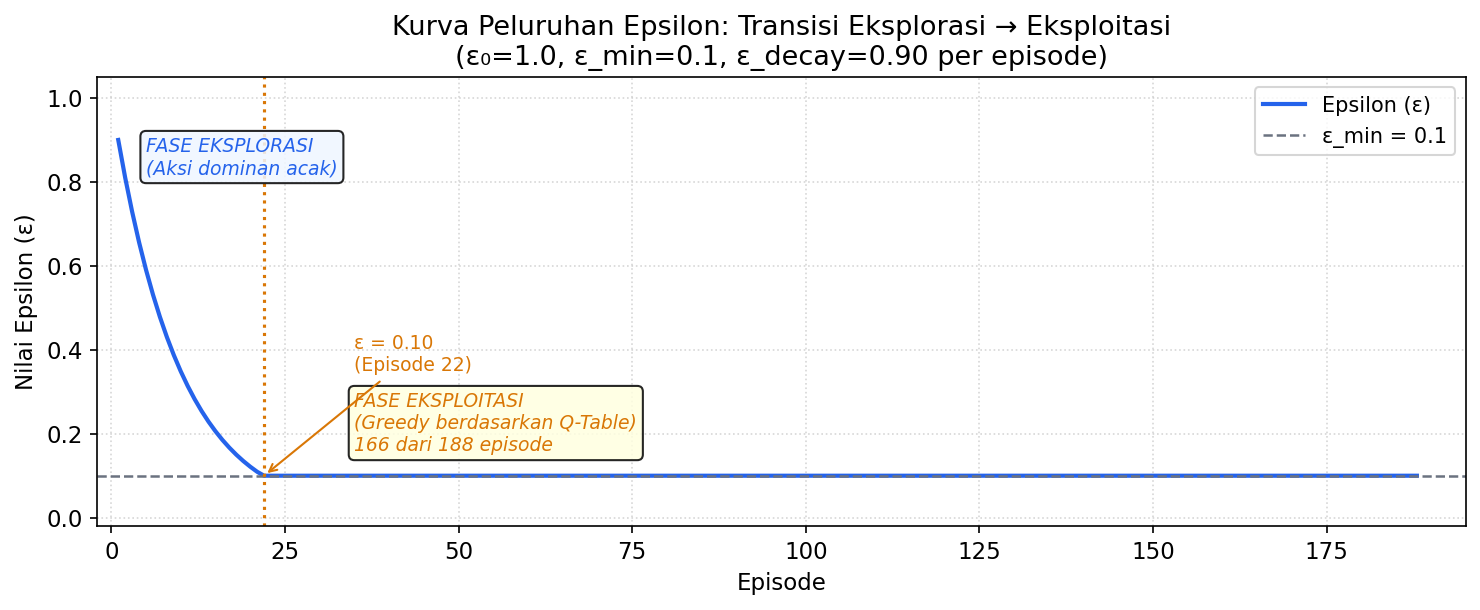
\includegraphics[width=0.85\textwidth]{gambar/epsilon_decay_ql.png} 
\caption{Kurva Peluruhan Epsilon ($\epsilon$-Greedy Decay) Agen Q-Learning}
\label{fig:epsilon_decay_ql}
\end{figure}

Berdasarkan analisis log lintasan aksi pada \texttt{log\_ql.csv}, proses pembelajaran agen secara garis besar terbagi ke dalam empat fase evolusi taktis. Dengan $\epsilon_{\text{decay}} = 0,90$, nilai $\epsilon$ menyentuh ambang minimum $0,10$ sekitar episode ke-22:
\begin{enumerate}
    \item \textbf{Fase 1: Rekognisi Stokastik (Episode 1--22):} Pada tahap ini, nilai $\epsilon$ masih di atas ambang minimum sehingga agen menyurvei berbagai \textit{endpoint} secara acak. Di fase ini, agen langsung berhasil mengidentifikasi celah-celah awal pada \textit{endpoint} 0 (\texttt{/search}) dan \textit{endpoint} 4 (\texttt{/login}). 
    \item \textbf{Fase 2: Eksploitasi Terarah Awal (Episode 23--300):} Setelah $\epsilon$ mencapai batas bawah ($0,10$), 90\% aksi dipilih berdasarkan $\arg\max Q(s,a)$. Agen secara intensif membombardir \textit{endpoint} 0 yang telah terbukti memberikan penguatan tinggi ($+50$). Setiap kali satu varian muatan SQLi atau XSS pada \textit{endpoint} 0 berhasil terverifikasi, aksi tersebut langsung di-mask, mendorong agen untuk mengeksploitasi muatan lain pada \textit{endpoint} yang sama. 
    \item \textbf{Fase 3: Pengalihan Ruang Serang dan Penemuan Celah Tersembunyi (Episode 301--787):} Setelah seluruh celah pada \textit{endpoint} 0 ter-mask, kebijakan $\arg\max$ agen terdorong beralih ke permukaan serang berikutnya. Di fase ini, agen berhasil menemukan 3 celah DOM XSS pada \textit{endpoint} 3 (\texttt{/track-order}) serta 3 kebocoran berkas \textit{poison null byte} pada \textit{endpoint} 1 (\texttt{/ftp/}). Seluruh 14 celah selesai dieksploitasi pada episode ke-787.
    \item \textbf{Fase 4: Kejenuhan Ruang Aksi dan Stabilitas Kebijakan (Episode 788--1.585):} Karena seluruh 14 aksi rentan telah di-mask permanen, agen tidak dapat lagi memperoleh reward $+50$. Agen terus mengeksplorasi sisa aksi yang ada dengan menerima umpan balik normal ($-1$). Stabilitas kurva pada fase ini membuktikan bahwa tidak terjadi osilasi kebijakan atau perilaku berulang yang merusak konvergensi.
\end{enumerate}

\subsection{Analisis Pertumbuhan Cumulative Reward dan Laju Efisiensi}

Dinamika akumulasi perolehan insentif agen Q-Learning sepanjang 1.585 episode interaksi divisualisasikan pada Gambar \ref{fig:cumulative_reward_ql}.

\begin{figure}[H]
\centering
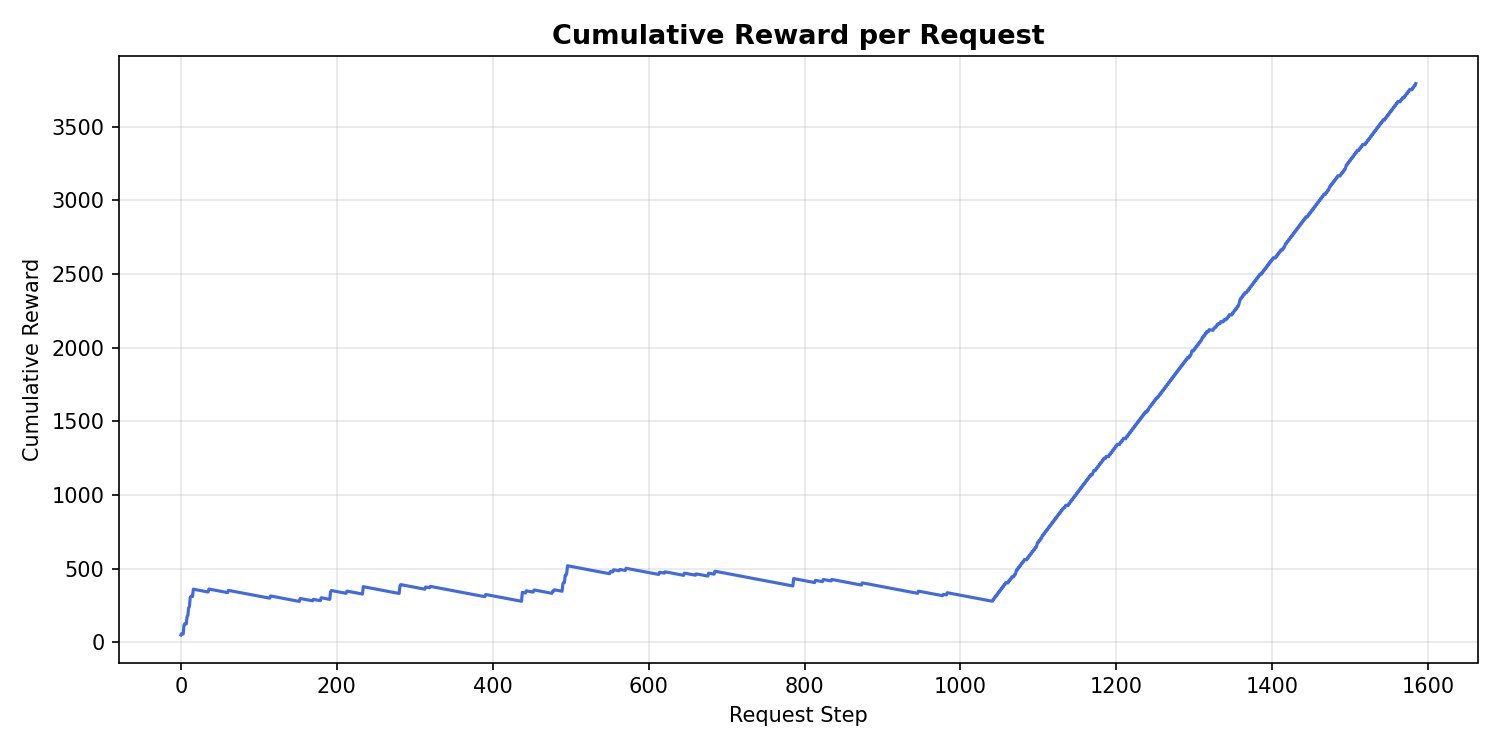
\includegraphics[width=0.85\textwidth]{gambar/cumulative_reward_ql.png} 
\caption{Kurva Pertumbuhan Cumulative Reward Q-Learning sepanjang 1.585 Episode}
\label{fig:cumulative_reward_ql}
\end{figure}

Kurva pada Gambar \ref{fig:cumulative_reward_ql} menunjukkan akumulasi reward hingga mencapai skor akhir \textbf{+3.783}. Lonjakan vertikal pada kurva berkorelasi langsung dengan episode di mana agen berhasil mengeksekusi celah keamanan baru ($+50$). Karakteristik kurva yang konsisten berada pada domain positif membuktikan bahwa insentif positif dari temuan kerentanan dan anomali jauh lebih dominan dibandingkan akumulasi penalti interaksi normal ($-1$). 

Laju akumulasi penemuan kerentanan disajikan pada Gambar \ref{fig:request_count_efficiency_ql}.

\begin{figure}[H]
\centering
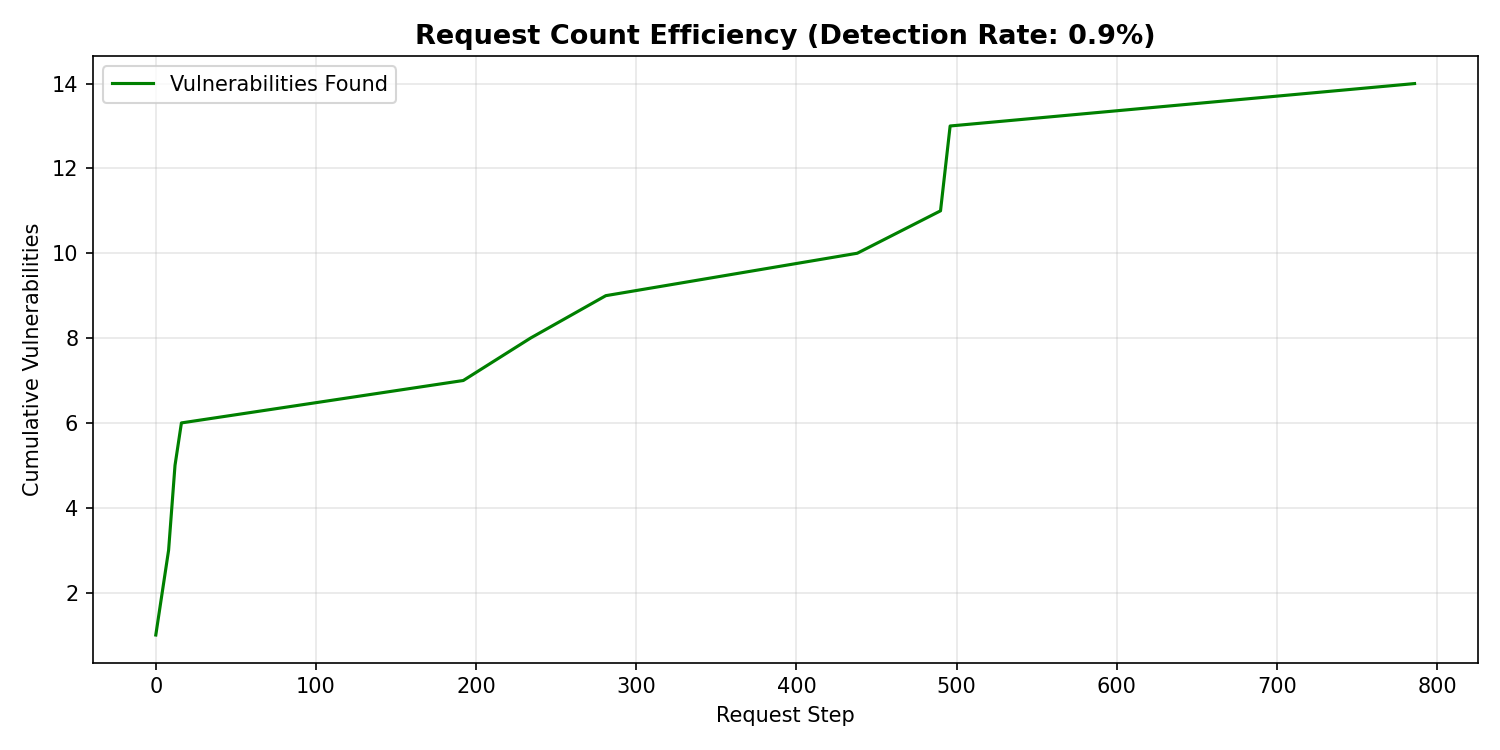
\includegraphics[width=0.85\textwidth]{gambar/request_count_efficiency_ql.png} 
\caption{Grafik Laju Penemuan Kerentanan Kumulatif Q-Learning (Efisiensi Request)}
\label{fig:request_count_efficiency_ql}
\end{figure}

Gambar \ref{fig:request_count_efficiency_ql} membuktikan bahwa agen Q-Learning tidak membutuhkan waktu pemanasan yang lama: celah pertama teridentifikasi pada \textbf{Episode 1}, dan seluruh 14 aksi rentan berhasil dituntaskan pada episode ke-787.

\subsection{Analisis Struktur Q-Table dan Nilai Q Tertinggi}

Sepanjang proses interaksi, agen Q-Learning memetakan lingkungan ke dalam \textbf{25 state unik} yang tercatat pada Q-Table. Tabel \ref{tab:qtable_top} menyajikan 10 nilai estimasi Q tertinggi yang dihasilkan pada akhir proses pelatihan. 

\begin{table}[H]
\centering
\caption{10 Nilai Q Tertinggi pada Q-Table Hasil Pelatihan Q-Learning}
\label{tab:qtable_top}
\begin{tabular}{|l|l|r|}
\hline
\textbf{Kondisi State} & \textbf{Aksi Terpilih (Payload@Endpoint)} & \textbf{Nilai Q} \\
\hline
\texttt{2xx|0|0|0|0|0|0|0} & \texttt{sqli\_comment@ep3} (\texttt{apple\textquotesingle --}) & 67,67 \\
\texttt{5xx|2|0|0|0|3|0|4} & \texttt{sqli\_login@ep0} (Bypass Login) & 59,18 \\
\texttt{2xx|0|0|0|0|6|0|0} & \texttt{sqli\_login@ep0} (Bypass Login) & 30,93 \\
\texttt{4xx|2|0|0|0|1|0|4} & \texttt{fuzz\_null@ep0} (\texttt{\%00}) & 30,89 \\
\texttt{4xx|1|0|0|0|1|0|4} & \texttt{sqli\_login@ep0} (Bypass Login) & 29,28 \\
\texttt{2xx|0|0|0|0|5|0|0} & \texttt{sqli\_login@ep0} (Bypass Login) & 29,04 \\
\texttt{4xx|0|0|0|0|4|0|4} & \texttt{fuzz\_null@ep1} (\texttt{\%00}) & 24,39 \\
\texttt{2xx|0|0|1|0|3|0|0} & \texttt{xss\_script@ep0} (\texttt{<script>}) & 14,94 \\
\texttt{2xx|2|0|1|0|2|0|0} & \texttt{sqli\_login@ep2} (Bypass Login) & 14,85 \\
\texttt{2xx|1|0|0|0|2|0|0} & \texttt{sqli\_login@ep0} (Bypass Login) & 11,69 \\
\hline
\end{tabular}
\end{table}

Nilai Q tertinggi yang tercatat pada tabel mencapai \textbf{67,67} pada \textit{state} \texttt{2xx|0|0|0|0|0|0|0}. Pola yang menonjol adalah dominasi aksi berbasis injeksi SQL seperti \texttt{sqli\_login@ep0} pada baris-baris teratas. Pola ini menunjukkan bahwa aksi tersebut memperoleh estimasi nilai tinggi pada state yang diamati. Interpretasi ini perlu dibaca bersama distribusi aksi dan hasil verifikasi, karena nilai Q sendiri bukan bukti kerentanan. Visualisasi peta panas (\textit{heatmap}) sebaran nilai Q pada seluruh pasangan \textit{state-action} disajikan pada Gambar \ref{fig:q_table_heatmap_ql}.

\begin{figure}[H]
\centering
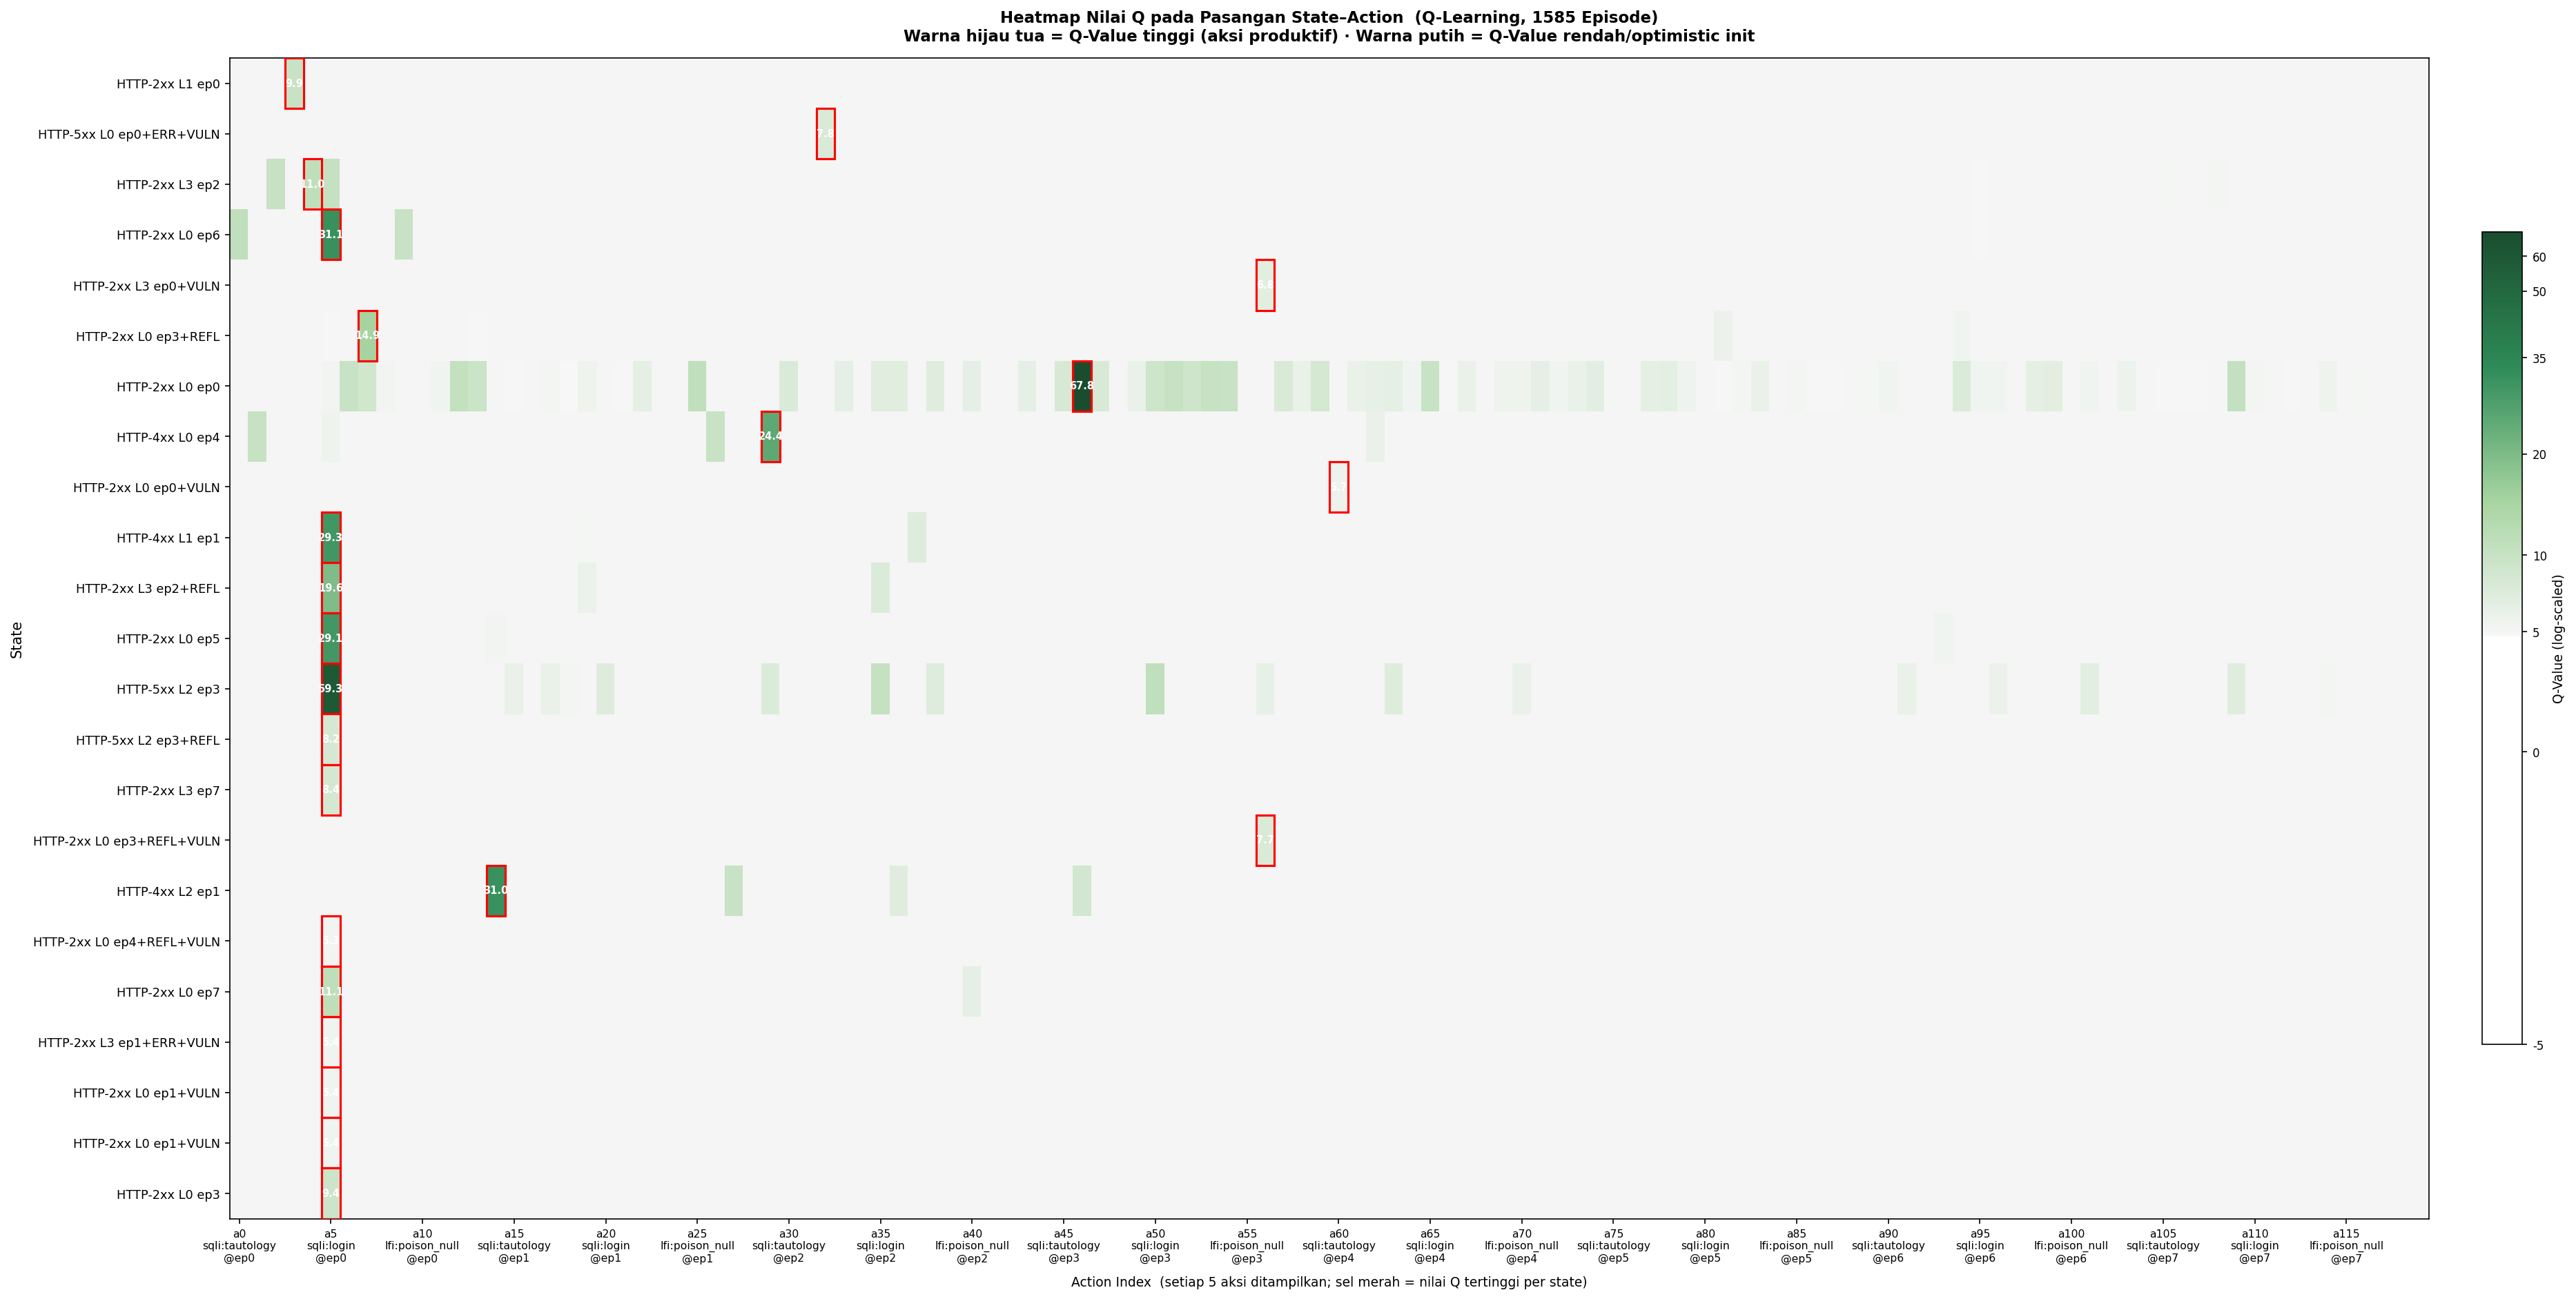
\includegraphics[width=0.95\textwidth]{gambar/q_table_heatmap_ql.png} 
\caption{Heatmap Matriks Q-Table: Pemetaan Nilai Aksi terhadap State Lingkungan}
\label{fig:q_table_heatmap_ql}
\end{figure}


\section{Evaluasi Komparatif: Tabular Q-Learning vs Deep Q-Network (DQN)}

\subsection{Perbandingan Kinerja Kuantitatif Q-Learning dan DQN}

Untuk memperkaya analisis kemampuan representasi kecerdasan buatan dalam pengetesan penetrasi web, sistem mengimplementasikan agen Deep Q-Network (DQN) sebagai pembanding terhadap agen tabular Q-Learning pada anggaran interaksi yang identik (1.585 episode). Tabel \ref{tab:comparison_ql_dqn} merangkum perbandingan kinerja kuantitatif antara kedua algoritma pemelajaran penguatan tersebut.

\begin{table}[htbp]
\centering
\caption{Perbandingan Kinerja Q-Learning vs Deep Q-Network (DQN)}
\label{tab:comparison_ql_dqn}
\small % Ukuran font proporsional
\setlength{\tabcolsep}{6pt} % Mengatur jarak antar kolom agar pas
\begin{tabular}{l c c}
\toprule
\textbf{Metrik Evaluasi} & \textbf{Tabular Q-Learning} & \textbf{Deep Q-Network (DQN)} \\
\midrule
Anggaran Permintaan Payload & 1.585 & 1.585 \\
Total Transaksi HTTP (\textit{w/ verifikasi}) & 1.639 & 1.636 \\ 
Kerentanan Terverifikasi Ditemukan & \textbf{14} & 13 \\ 
Jumlah Lokasi Kerentanan Unik & 5 & 5 \\
SQL Injection & 6 & 6 \\
Reflected XSS (DOM Verified) & 5 & 5 \\ 
Fuzzing / File Disclosure & 3 & 2 \\
Akumulasi Insentif (\textit{Cumulative Reward}) & 3.783 & \textbf{9.503} \\ 
Tingkat Keberhasilan (\textit{Vuln Hit Rate}) & 0,88\% & 0,76\% \\ 
Rasio Permintaan per Kerentanan & \textbf{113,21} & 121,92 \\ 
Episode Penemuan Pertama & Episode 1 & Episode 1 \\
Episode Seluruh Temuan Dikuasai & Episode 787 & \textbf{Episode 443} \\
Waktu Eksekusi Pelatihan & \textbf{142,55 detik} & 146,95 detik \\ 
\bottomrule
\end{tabular}
\end{table}

\subsection{Analisis Kemampuan Generalisasi Nilai dan Akumulasi Reward}

Data pada Tabel \ref{tab:comparison_ql_dqn} memperlihatkan perbedaan fundamental antara pendekatan tabular dan aproksimasi fungsi berbasis jaringan saraf tiruan:
\begin{enumerate}
    \item \textbf{Kecepatan Penemuan Kerentanan:} DQN berhasil mengidentifikasi seluruh 13 kerentanan yang ditemukannya (6 SQLi, 5 XSS, 2 Fuzz) secara jauh lebih cepat, yaitu pada \textbf{Episode 443}, dibandingkan Q-Learning yang membutuhkan 787 episode untuk menemukan 14 kerentanan. Hal ini dimungkinkan oleh kemampuan aproksimasi fungsi jaringan saraf yang mampu melakukan generalisasi nilai (\textit{value generalization}) lintas ruang \textit{state} vektor 28 dimensi. Ketika jaringan mempelajari bahwa suatu vektor input mencirikan anomali, bobot jaringan secara serempak memperbarui estimasi nilai untuk state-state berdekatan. 
    \item \textbf{Akumulasi Reward (+9.503 vs +3.783):} DQN mencatatkan perolehan \textit{cumulative reward} sekitar 2,51 kali lipat lebih besar dibanding Q-Learning. Mekanisme memori pengalaman (\textit{experience replay buffer}) berkapasitas 10.000 transisi memungkinkan sampel pengalaman berinsentif tinggi dilatih berulang kali (\textit{mini-batch sampling}) ke dalam bobot jaringan saraf, menjaga stabilitas estimasi nilai positif sepanjang proses pelatihan. 
\end{enumerate}

\subsection{Analisis Perbedaan Pola Eksplorasi: Konsentrasi vs Distribusi Merata}

Perbedaan yang sangat kontras juga tampak pada profil distribusi permintaan antar-\textit{endpoint}:
\begin{itemize}
    \item \textbf{Q-Learning Tabular:} Sangat terkonsentrasi secara tajam pada \textit{endpoint} 0 (1.184 dari 1.585 \textit{request}, atau 74,7\%). Tabel lookup Q-Learning memperbarui nilai secara terisolasi per sel $(s, a)$, sehingga begitu satu sel memperoleh nilai sangat tinggi, agen cenderung terus mengeksploitasi sel tersebut pada state aktif. 
    \item \textbf{Deep Q-Network (DQN):} Mengalokasikan permintaan yang jauh lebih tersebar dan merata di seluruh 8 \textit{endpoint} (berkisar antara 73 hingga 377 \textit{request} per \textit{endpoint}). Hal ini dipengaruhi oleh laju peluruhan eksplorasi yang lebih landai ($\epsilon_{\text{decay}} = 0,9965$) yang mempertahankan tingkat eksplorasi aktif hingga episode ke-1.000. 
\end{itemize}

Grafik kurva pertumbuhan insentif dan laju efisiensi DQN masing-masing disajikan pada Gambar \ref{fig:cumulative_reward_dqn} dan Gambar \ref{fig:request_count_efficiency_dqn}.

\begin{figure}[H]
\centering
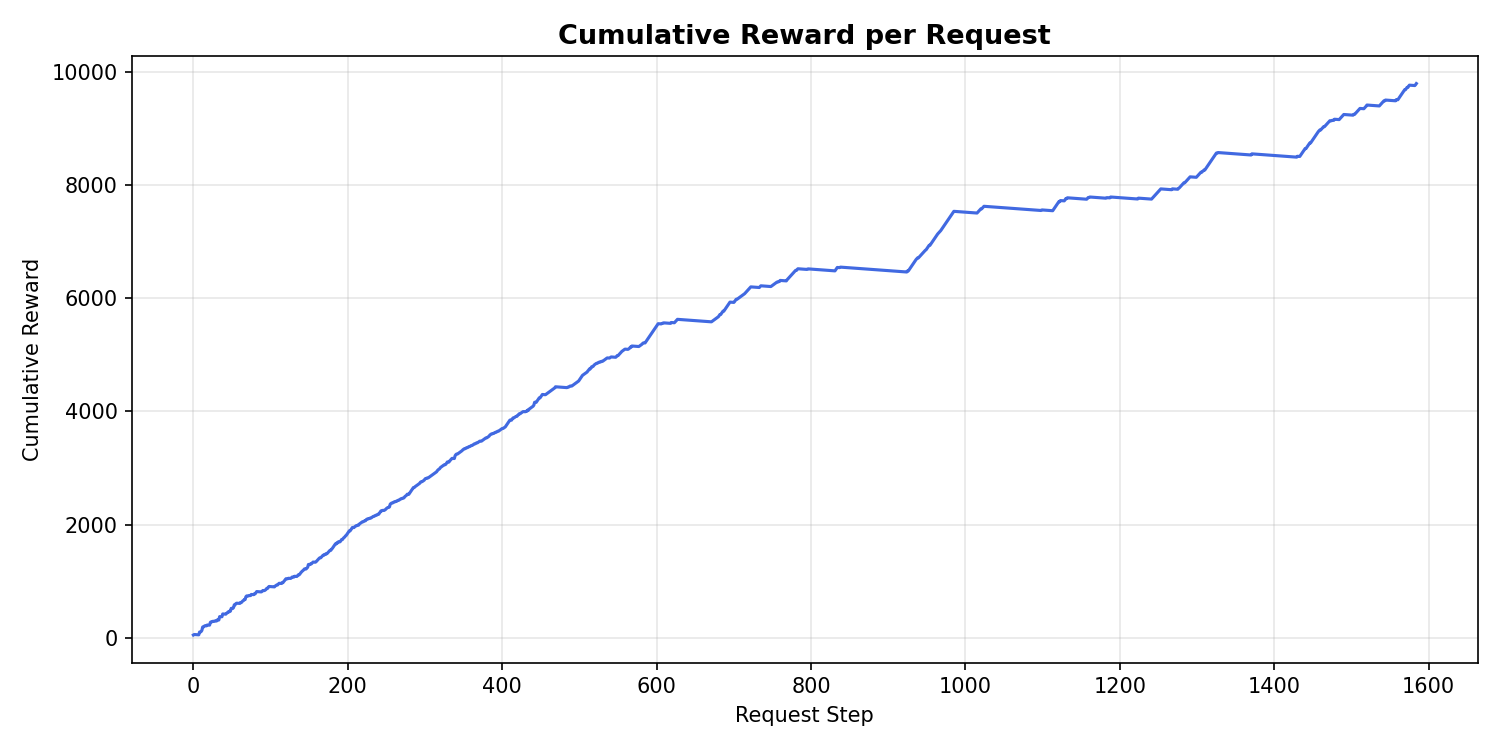
\includegraphics[width=0.85\textwidth]{gambar/cumulative_reward_dqn.png} 
\caption{Kurva Pertumbuhan Cumulative Reward Deep Q-Network (DQN)}
\label{fig:cumulative_reward_dqn}
\end{figure}

\begin{figure}[H]
\centering
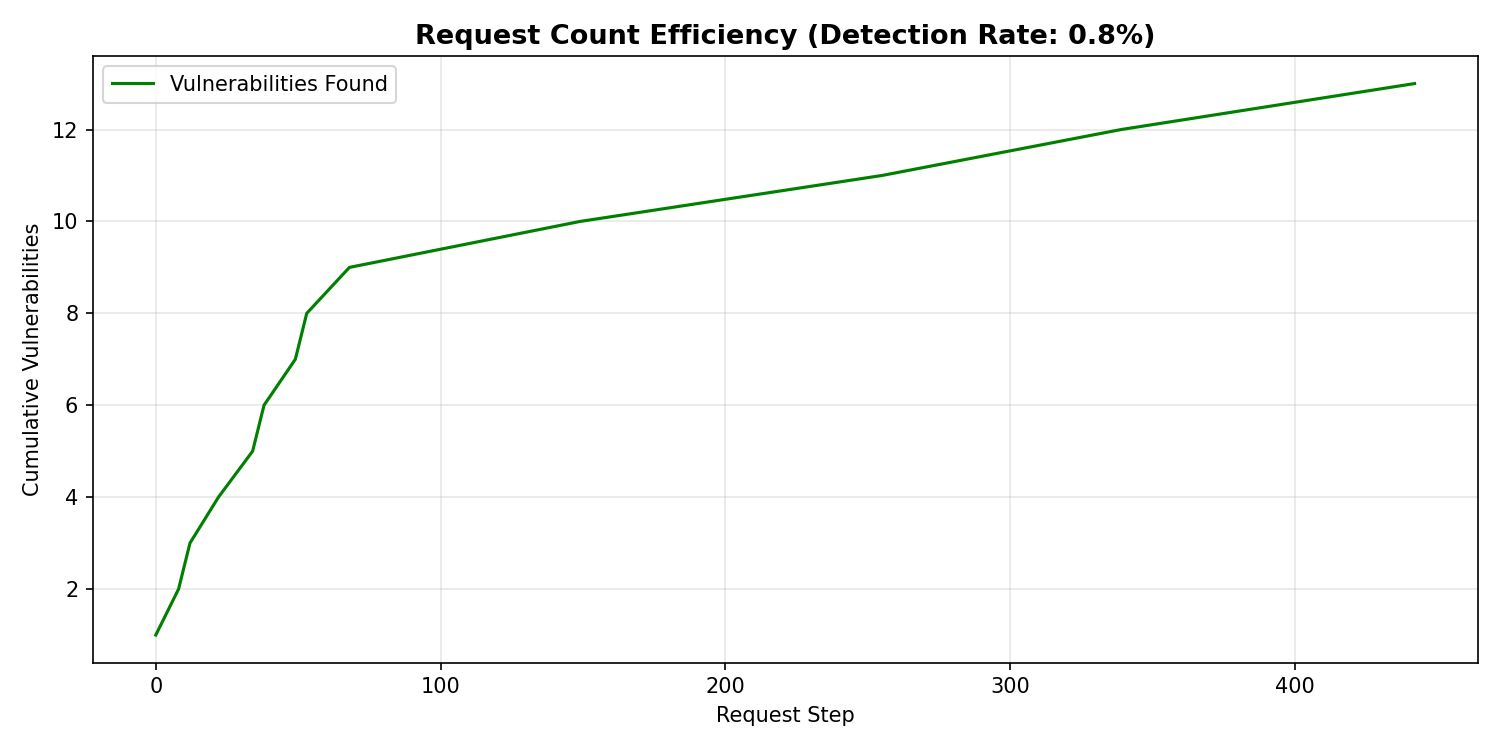
\includegraphics[width=0.85\textwidth]{gambar/request_count_efficiency_dqn.png} 
\caption{Grafik Laju Penemuan Kerentanan Kumulatif Deep Q-Network (DQN)}
\label{fig:request_count_efficiency_dqn}
\end{figure}

\text Hasil menunjukkan perbedaan kinerja pada run yang diamati. Q-Learning menemukan 14 aksi terverifikasi (7 SQLi, 5 XSS, 2 Fuzz), sedangkan DQN menemukan 13 aksi (6 SQLi, 5 XSS, 2 Fuzz). DQN mencapai seluruh temuan yang diperolehnya pada episode ke-443, sementara Q-Learning mencapai 14 temuan pada episode ke-787. Reward kumulatif masing-masing adalah 3.783 dan 9.503. Nilai reward yang lebih tinggi tidak dengan sendirinya menunjukkan deteksi yang lebih baik; hasil ini perlu dibaca bersama jumlah temuan, anggaran request, serta sifat evaluasi yang in-sample. Durasi pelatihan yang tercatat masing-masing 142,55 detik dan 146,95 detik pada run ini.
\section{Perbandingan dengan OWASP ZAP}

\subsection{Rincian Arsitektur dan Prosedur Pemindaian OWASP ZAP}

Pada eksperimen ini, OWASP ZAP dijalankan sebagai daemon yang dikendalikan melalui API oleh skrip Python. Alurnya terdiri atas pengendali eksperimen, API ZAP, mesin pemindaian, aplikasi target, dan pengolahan alert. Pengendali menentukan URL dan tahapan pemindaian. Mesin ZAP menjalankan akses URL, spider, serta pemindaian aktif. Hasil pesan dan alert kemudian diambil kembali oleh pengendali untuk dihitung menggunakan kriteria penelitian.

\begin{enumerate}
    \item \textbf{Pengendali Python:} menetapkan dua URL dalam cakupan, memeriksa versi ZAP, mencatat jumlah pesan awal, dan mengirim perintah melalui API.
    \item \textbf{Core API ZAP:} menyediakan operasi untuk mengakses URL, memulai spider dan pemindaian aktif, membaca status proses, mengambil riwayat pesan, serta mengambil alert.
    \item \textbf{Akses URL dan spider:} setiap URL diakses terlebih dahulu. Spider kemudian menelusuri sumber daya yang dapat dijangkau dan statusnya diperiksa secara berkala sampai proses selesai.
    \item \textbf{Pemindaian aktif:} setelah spider selesai, pemindaian aktif dijalankan dengan \texttt{recurse=false}. ZAP mengirimkan permintaan uji sesuai aturan dan konfigurasi pemindainya.
    \item \textbf{Pengumpulan hasil:} setelah setiap tahap, skrip membaca jumlah pesan dan menghitung selisihnya terhadap jumlah sebelum tahap tersebut. Setelah pemindaian selesai, skrip mengambil alert melalui API.
    \item \textbf{Penyaringan untuk analisis:} alert dikelompokkan menurut kategori penelitian. Hanya alert SQLi, XSS, atau path traversal dengan risiko High atau Medium yang dihitung sebagai temuan relevan.
\end{enumerate}

Untuk memberikan representasi visual yang jelas mengenai interaksi sistem, hubungan komponen arsitektur modular OWASP ZAP beserta alur prosedur pemindaian yang dikendalikan oleh skrip pengendali Python tersebut dimodelkan pada Gambar \ref{fig:zap_architecture_flow}.

\begin{figure}[H]
\centering
% Memaksa seluruh diagram mengecil secara otomatis mengikuti lebar teks halaman dokumen
\resizebox{\textwidth}{!}{
\begin{tikzpicture}[
    font=\sffamily\small,
    node distance=1.2cm and 1.5cm,
    % Definisi Gaya Kotak Komponen
    core/.style={rectangle, rounded corners, draw=blue!70, fill=blue!10, thick, minimum width=3.3cm, minimum height=1.1cm, align=center},
    scanner/.style={rectangle, rounded corners, draw=orange!70, fill=orange!10, thick, minimum width=3.3cm, minimum height=1.1cm, align=center},
    db/.style={cylinder, draw=gray!70, fill=gray!20, thick, shape border rotate=90, minimum width=2.2cm, minimum height=1.6cm, align=center},
    external/.style={rectangle, draw=green!70!black, fill=green!5, thick, minimum width=3.3cm, minimum height=1.1cm, align=center},
    % Definisi Gaya Garis Panah
    arrow/.style={- {Stealth[scale=1.2]}, thick, draw=gray!80},
    doublearrow/.style={{Stealth[scale=1.2]} - {Stealth[scale=1.2]}, thick, draw=gray!80}
]

    % --- LAYER 1: PENGENDALI PYTHON ---
    \node[external] (python) {\textbf{1. Pengendali Python}\\(Skrip Eksperimen)};
    
    % --- LAYER 2: INTERFACES ZAP ---
    \node[core] (api) [right=2.2cm of python] {\textbf{2. Core API ZAP}\\(Endpoint Operasi)};
    \node[core] (engine) [right=1.2cm of api] {\textbf{ZAP Core Engine}\\(Orkestrator Sesi)};

    % --- LAYER 3: PROSEDUR PEMINDAIAN ---
    \node[scanner] (spider) [above right=0.4cm and 1.2cm of engine] {\textbf{3. Akses \& Spider}\\(Pemetaan Direktori)};
    \node[scanner] (active) [below right=0.4cm and 1.2cm of engine] {\textbf{4. Pemindaian Aktif}\\(Active Scanner)};

    % --- LAYER 4: TARGET & REPOSITORI ALERTS ---
    \node[external] (target) [right=4.2cm of engine] {\textbf{Aplikasi Target}\\(Subset 2 Endpoint)};
    \node[db] (database) [below=1.4cm of engine] {\textbf{5 \& 6. Filter Alerts}\\(High / Medium Only)};

    % --- ALUR DATA DAN HUBUNGAN ANTAR KOMPONEN ---
    % Pengendali mengirim perintah ke API
    \draw[arrow] (python) -- node[above, font=\footnotesize] {Kendalikan} 
                            node[below, font=\footnotesize] {Skrip API} (api);
    
    % API meneruskan ke Core Engine ZAP
    \draw[doublearrow] (api) -- (engine);
    
    % Core Engine menggerakkan tahapan operasional
    \draw[arrow] (engine) |- (spider);
    \draw[arrow] (engine) |- (active);
    
    % Aktivitas pemindaian dari modul ke target
    \draw[arrow] (spider) -| node[pos=0.4, above, font=\footnotesize] {Akses URL} (target);
    \draw[arrow] (active) -| node[pos=0.4, below, font=\footnotesize] {1.585 Request} (target);
    
    % Pengumpulan kembali hasil alert ke database
    \draw[arrow] (engine) -- (database);
    
    % Alur pengambilan temuan kembali ke skrip python pengendali
    \draw[arrow] (database) -| node[pos=0.8, left, font=\footnotesize, xshift=-0.2cm] {Ambil Temuan} (python);

\end{tikzpicture}
} % Akhir penutup \resizebox
\caption{Rincian Arsitektur Integrasi Pengendali Python dan Prosedur Pemindaian OWASP ZAP}
\label{fig:zap_architecture_flow}
\end{figure}



Pemindai pasif ZAP menganalisis pesan yang diamati tanpa mengubah pesan, sedangkan pemindai aktif mengirimkan probe ke target. Skrip eksperimen secara eksplisit menjalankan akses URL, spider, dan pemindaian aktif; skrip tidak memulai pekerjaan pemindaian pasif tersendiri. Alert yang tidak masuk kriteria perbandingan tetap merupakan keluaran ZAP, tetapi tidak dihitung sebagai temuan relevan dalam metrik penelitian.

Laporan pemindaian terkontrol yang digunakan mencatat ZAP versi 2.17.0 dan menghasilkan total akumulasi lalu lintas komunikasi sebanyak 1.585 request pesan pada target yang mencakup aktivitas pemetaan akses URL, spider, serta eksekusi pemindaian aktif. Dari seluruh rangkaian aktivitas tersebut, ZAP menghasilkan 32 alert mentah di mana terdapat dua alert yang memenuhi kriteria batas risiko High atau Medium untuk dihitung ke dalam temuan relevan perbandingan. Pengklasifikasian ini wajib dipastikan konsistensinya di sepanjang penyebutan metrik ZAP pada Bab 4.

Pada subset dua endpoint yang sama, QL mencatat 1.214 permintaan payload untuk 10 temuan, sedangkan ZAP mencatat total 1.585 request pesan untuk menghasilkan dua temuan relevan. Cakupan endpoint yang sama tidak membuat prosedur kedua metode sepenuhnya setara. QL memilih payload satu per satu melalui kebijakan agen, sedangkan ZAP menjalankan alur akses URL, spider, dan pemindaian aktif. Karena strategi dan cara penghitungan request berbeda, rasio request per temuan hanya bersifat deskriptif untuk eksperimen ini.

Perbandingan dengan OWASP ZAP dilakukan menggunakan hasil pemindaian terkontrol pada dua endpoint, yaitu \texttt{/rest/products/search?q=} dan \texttt{/ftp/}. Untuk membatasi perbedaan cakupan, hasil Q-Learning juga dihitung pada subset dua endpoint tersebut. Ringkasan perbandingan ditampilkan pada Tabel \ref{tab:zap_comparison}.

\begin{table}[H]
\centering
\caption{Perbandingan Hasil Q-Learning dan OWASP ZAP pada Dua Endpoint}
\label{tab:zap_comparison}
\begin{tabular}{|l|c|c|}
\hline
\textbf{Metrik} & \textbf{Q-Learning (subset)} & \textbf{OWASP ZAP} \\
\hline
Endpoint yang dicakup & 2 & 2 \\
Jumlah request & 1.226 & 1.585 \\
Temuan relevan yang dihitung & 10 & 2 \\
SQL Injection & 5 & 1 \\
Reflected XSS & 2 & 1 \\
Fuzzing / anomali file & 3 & 0 \\
Request per temuan & 122,60 & 792,50 \\
\hline
\end{tabular}
\end{table}

Pada subset tersebut, rasio request per temuan Q-Learning adalah 122,60, sedangkan OWASP ZAP sebesar 792,50. Rasio kedua nilai tersebut sekitar 6,46. Angka ini menggambarkan hasil pada konfigurasi dan run yang digunakan dalam penelitian, bukan bukti bahwa Q-Learning secara umum 6,46 kali lebih efisien. ZAP dan Q-Learning menggunakan strategi pemindaian serta kumpulan payload yang berbeda. Karena itu, perbandingan ini bersifat deskriptif dan perlu ditafsirkan dengan mempertimbangkan perbedaan metode.

OWASP ZAP menghasilkan 32 alert mentah; dua alert masuk kategori yang dihitung sebagai temuan relevan dalam laporan perbandingan, yaitu satu SQL Injection dan satu Reflected XSS. Alert lainnya tidak dimasukkan ke hitungan kerentanan aktif pada penelitian ini. Gambar \ref{fig:vuln_breakdown} menyajikan distribusi temuan berdasarkan kategori.

\begin{figure}[H]
\centering
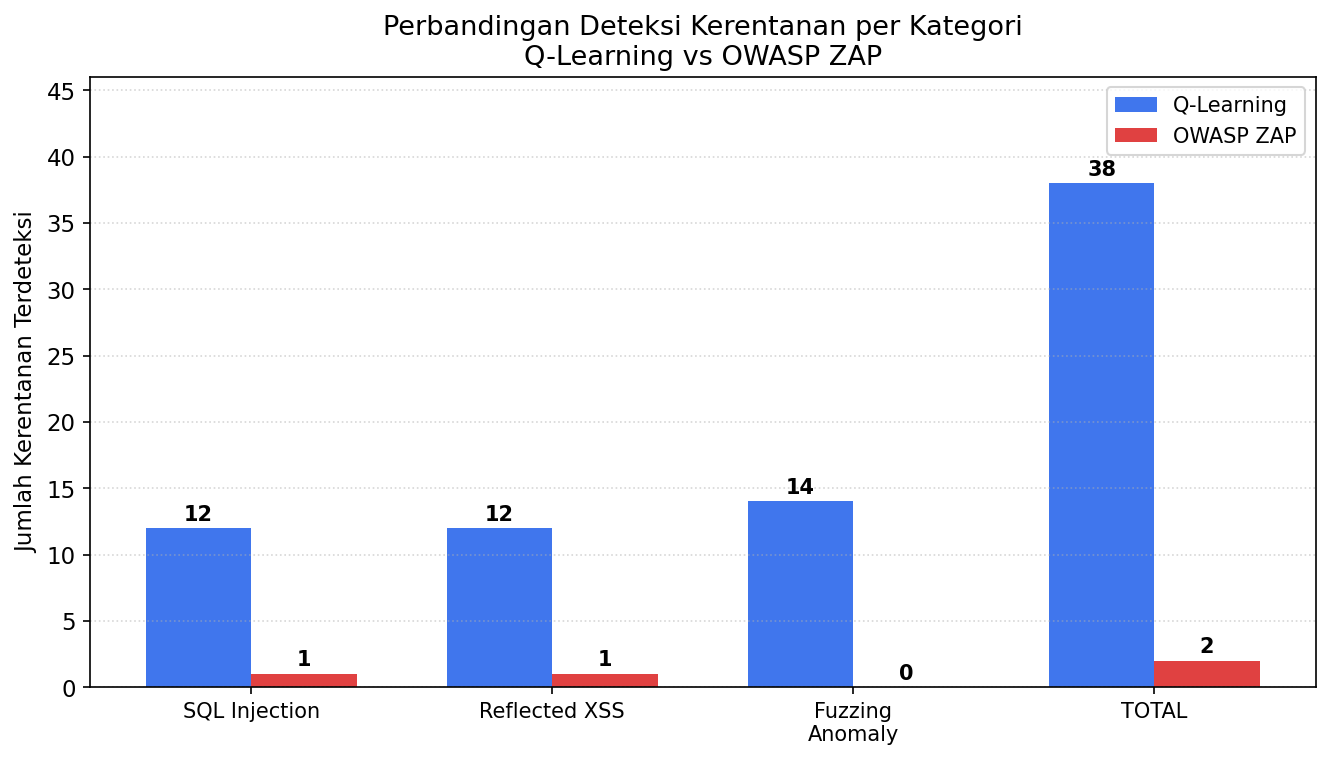
\includegraphics[width=0.85\textwidth]{gambar/vuln_breakdown_ql_zap.png}
\caption{Distribusi Temuan Relevan Q-Learning dan OWASP ZAP}
\label{fig:vuln_breakdown}
\end{figure}



\section{Keterbatasan Penelitian}

Hasil penelitian ini memiliki beberapa batasan. Pertama, metrik Q-Learning dan DQN bersifat \textit{in-sample}: metrik dihitung dari episode yang juga digunakan selama pelatihan. Oleh sebab itu, hasil belum mengukur kemampuan generalisasi kebijakan pada data uji terpisah maupun aplikasi web lain. Kedua, percobaan yang dilaporkan menggunakan satu nilai \textit{random seed}; variasi antar-run belum dianalisis sehingga perbedaan kinerja belum dapat dinyatakan signifikan secara statistik.

Ketiga, daftar payload dan pemetaan \textit{surface} disusun dengan pengetahuan tentang struktur OWASP Juice Shop. Hal ini merupakan \textit{human prior} yang perlu dinyatakan sebagai bagian dari metode penelitian. Keempat, label ground truth dan mekanisme verifikasi memakai bukti teknis yang sejenis dengan sistem, sehingga benchmark detektor tidak sepenuhnya independen. Hasil benchmark sebaiknya dipahami sebagai konsistensi terhadap ground truth terkurasi, bukan bukti akurasi universal.

Kelima, perbandingan dengan OWASP ZAP hanya mencakup dua endpoint dan menggunakan strategi pemindaian yang berbeda. Jumlah request dan temuan karena itu tidak sepenuhnya setara. Penelitian lanjutan dapat mengulang eksperimen dengan beberapa seed, menyediakan evaluasi held-out, menguji target tambahan, dan menyamakan prosedur penghitungan request serta temuan.

Pada eksperimen yang dilakukan, Q-Learning memperoleh 14 temuan terverifikasi dan DQN memperoleh 13 temuan terverifikasi dari anggaran masing-masing 1.585 request payload. Benchmark detektor pada 120 aksi menghasilkan 13 \textit{true positive}, 1 \textit{false negative}, 0 \textit{false positive} pada 60 aksi berlabel negatif, serta 46 aksi berstatus \textit{unknown}. Perbandingan terbatas pada dua endpoint menunjukkan 10 temuan Q-Learning dan 2 temuan ZAP, tetapi perbedaan metode pemindaian membatasi kesimpulan efisiensi yang dapat ditarik. Seluruh hasil tersebut berlaku pada lingkungan dan konfigurasi penelitian ini.


 % ini file bab 4. 
% Edit di file 07_bab4.tex
% jika bab ini tidak dipakai, bisa di-comment (tambah simbol % di depan)

\chapter{Kesimpulan dan Saran}

\section{Kesimpulan}

Berdasarkan perancangan, implementasi, dan pengujian sistem \textit{automated web penetration testing} berbasis \textit{Reinforcement Learning} pada aplikasi OWASP Juice Shop, kesimpulan penelitian ini adalah sebagai berikut.

\begin{enumerate}
    \item Sistem pengujian penetrasi web berbasis \textit{Reinforcement Learning} berhasil diimplementasikan dengan mengintegrasikan agen, pembangkit \textit{payload}, klien HTTP, penganalisis respons, mekanisme verifikasi, dan pencatatan hasil. Pengujian menggunakan delapan \textit{endpoint} dan 15 \textit{payload}, sehingga terdapat 120 kombinasi aksi yang menjadi ruang pengujian. Sistem juga menerapkan verifikasi kontrol-diferensial untuk kandidat SQL Injection dan \textit{fuzzing}, serta verifikasi eksekusi pada DOM menggunakan peramban untuk kandidat XSS.

    \item Dengan anggaran masing-masing 1.585 episode, Q-Learning memperoleh 14 aksi dengan kerentanan terverifikasi, sedangkan DQN memperoleh 12. Temuan Q-Learning terdiri atas enam SQL Injection, lima XSS terverifikasi pada DOM, dan tiga temuan \textit{fuzzing} atau pengungkapan berkas. Temuan DQN terdiri atas enam SQL Injection, empat XSS terverifikasi pada DOM, dan dua temuan \textit{fuzzing} atau pengungkapan berkas. Kedua agen mencapai lima lokasi kerentanan unik, yang dihitung sebagai pasangan \textit{endpoint} dan kelas kerentanan. Pada \textit{run} yang diamati, \textit{vuln hit rate} Q-Learning adalah 0,88\% dan DQN 0,76\%.

    \item Pola hasil kedua agen menunjukkan perbedaan pada beberapa aspek. Q-Learning memperoleh lebih banyak aksi terverifikasi, sedangkan DQN mencapai seluruh temuan yang akhirnya diperolehnya pada episode ke-443, dibandingkan episode ke-787 pada Q-Learning. DQN juga menghasilkan \textit{cumulative reward} yang lebih tinggi, yaitu 10.209 dibandingkan 3.785. Namun, nilai \textit{reward} yang lebih tinggi tidak dengan sendirinya menunjukkan deteksi yang lebih baik; hasil perlu dinilai bersama jumlah temuan terverifikasi, efisiensi permintaan, dan karakteristik fungsi \textit{reward}. Perbandingan ini terbatas pada satu \textit{run} dan tidak menunjukkan keunggulan umum salah satu algoritma.

    \item Evaluasi detektor terhadap 120 aksi menghasilkan 13 \textit{true positive}, satu \textit{false negative}, dan nol \textit{false positive} pada 60 aksi yang berlabel negatif. Sebanyak 46 aksi lainnya berstatus \textit{unknown} dan tidak digunakan sebagai label negatif. Hasil tersebut menunjukkan konsistensi detektor terhadap \textit{ground truth} terkurasi dalam pengujian ini. Hasil ini tidak dapat dianggap sebagai bukti akurasi universal karena label dan mekanisme verifikasi menggunakan bukti teknis yang sejenis.

    \item Pada perbandingan terbatas di dua \textit{endpoint} yang sama, Q-Learning memperoleh 10 temuan relevan dan OWASP ZAP memperoleh dua temuan relevan. Hasil ini bersifat deskriptif karena strategi pemindaian dan cara penghitungan permintaan kedua sistem berbeda. Oleh karena itu, hasil tersebut belum cukup untuk menyimpulkan bahwa salah satu sistem secara umum lebih efisien daripada sistem lainnya.

    \item Evaluasi kinerja agen dalam penelitian ini bersifat \textit{in-sample}, karena metrik dihitung dari episode yang juga digunakan selama pelatihan. Pengujian juga dilakukan pada satu aplikasi target dan satu nilai \textit{random seed}. Dengan demikian, hasil penelitian menggambarkan kinerja sistem pada lingkungan dan konfigurasi yang digunakan, tetapi belum mengukur generalisasi pada data uji terpisah, target lain, atau variasi antar-\textit{run}.
\end{enumerate}

\section{Saran}

Berdasarkan hasil dan keterbatasan penelitian, beberapa saran untuk pengembangan selanjutnya adalah sebagai berikut.

\begin{enumerate}
    \item Penelitian selanjutnya disarankan menjalankan eksperimen menggunakan beberapa nilai \textit{random seed}. Hasil dapat dilaporkan dalam bentuk rata-rata dan variasi antar-\textit{run} agar kestabilan kinerja Q-Learning dan DQN dapat dibandingkan dengan lebih memadai. Evaluasi pada episode atau kumpulan aksi yang tidak digunakan selama pelatihan juga diperlukan untuk mengukur kemampuan generalisasi.

    \item Pengujian dapat diperluas ke aplikasi web lain, lebih banyak \textit{endpoint}, dan variasi teknologi di sisi server. Perluasan ini dapat membantu menilai apakah sistem mampu beradaptasi pada lingkungan yang karakteristiknya berbeda dari OWASP Juice Shop.

    \item Penyusunan \textit{ground truth} sebaiknya diperkuat melalui pemeriksaan independen dan dokumentasi bukti untuk setiap aksi. Aksi berlabel \textit{unknown} perlu tetap dipisahkan dari aksi negatif, atau diperiksa lebih lanjut, agar evaluasi tidak menganggap aksi yang belum diketahui sebagai aksi yang aman.

    \item Perbandingan dengan OWASP ZAP dapat dikembangkan dengan menyamakan cakupan target, definisi temuan, dan aturan penghitungan permintaan sejauh memungkinkan. Aktivitas seperti akses URL, \textit{spider}, dan pemindaian aktif sebaiknya dicatat secara terpisah agar batas perbandingan dapat dijelaskan dengan lebih terukur.

    \item Pengembangan berikutnya dapat menguji pengaruh variasi \textit{hyperparameter} dan fungsi \textit{reward} terhadap pola eksplorasi, jumlah temuan terverifikasi, serta jumlah permintaan yang diperlukan. Evaluasi sebaiknya tidak hanya mengandalkan \textit{cumulative reward}, tetapi juga melaporkan temuan terverifikasi dan efisiensi permintaan secara bersamaan.

    \item Untuk penerapan di luar lingkungan lokal penelitian, pengujian perlu dilakukan hanya pada sistem yang telah mendapat izin. Penggunaan pembatasan laju permintaan, pencatatan aktivitas, dan lingkungan uji terisolasi dapat membantu menjaga agar proses evaluasi tetap terkendali.
\end{enumerate}

%==============================================================
\renewcommand{\bibname}{Daftar Pustaka} % nama bab daftar pustaka
\addcontentsline{toc}{chapter}{Daftar Pustaka}
\bibliographystyle{apacite} % APA style
\bibliography{08_daftar-pustaka} % file bibtex berisi daftar referensi. 
% Isi referensi anda di file 08_daftar-pustaka.bib, dengan format bibtex.

%==============================================================
\appendix
\thispagestyle{empty}
\null
\vspace*{\fill}
\begin{center}
    {\LARGE \textbf{LAMPIRAN}}
\end{center}
\addcontentsline{toc}{chapter}{Lampiran} 
\vspace*{\fill}
\clearpage
\pagestyle{plain}

\chapter{Komentar Penguji dan Respon terhadap Komentar}

\section*{1. Komentar Pak Helmy}
\textbf{Komentar:} \\
Rumusan masalah pertama dibuat lebih lugas dan langsung menyebutkan permasalahan utama yang berkaitan dengan Reinforcement Learning.

\textbf{Respon:} \\
Rumusan masalah telah direvisi dengan menggunakan kalimat yang lebih lugas dan berfokus langsung pada penerapan \textit{Reinforcement Learning} dalam sistem \textit{automated web penetration testing}. Perubahan dilakukan pada bagian \textit{Rumusan Masalah} di Bab I. Kalimat sebelumnya yang terlalu panjang dan umum telah diganti menjadi pembahasan yang lebih spesifik mengenai penerapan RL untuk menentukan strategi pengujian kerentanan secara adaptif.

\vspace{0.5cm}

\section*{2. Komentar Pak Helmy}
\textbf{Komentar:} \\
Pada metode penelitian, skenario pengujian dibuat lebih detail.

\textbf{Respon:} \\
Bagian metode penelitian telah diperbaiki dengan menambahkan penjelasan yang lebih rinci mengenai skenario pengujian. Revisi mencakup penjelasan environment yang digunakan, definisi \textit{state}, \textit{action}, \textit{reward}, parameter \textit{Reinforcement Learning}, serta metode evaluasi sistem. Perubahan dapat dilihat pada Bab III bagian \textit{Metode Penelitian} dan subbab \textit{Skenario Pengujian Sistem}.

\vspace{0.5cm}

\section*{3. Komentar Pak Helmy}
\textbf{Komentar:} \\
Penelitian terkait nomor 8 kosong, dilengkapi atau dihapus apabila memang tidak ada.

\textbf{Respon:} \\
Bagian penelitian terkait yang kosong telah ada, dikarenakan kesalahan teknis yang ada sehingga bagian tersebut bisa hilang. Perubahan dapat dilihat pada Bab II bagian \textit{Penelitian Terdahulu}.

\vspace{0.5cm}

\section*{4. Komentar Pak Helmy}
\textbf{Komentar:} \\
Pembahasan yang dikerjakan banyak, tetapi isi pembahasannya masih terlalu sedikit.

\textbf{Respon:} \\
Isi pembahasan telah diperluas dengan menambahkan penjelasan teknis yang lebih mendalam terkait proses \textit{Reinforcement Learning}, mekanisme pengujian otomatis, serta integrasi sistem dengan OWASP Juice Shop. Selain itu, beberapa subbab yang terlalu singkat telah digabung agar pembahasan menjadi lebih fokus dan substantif. Perubahan dapat dilihat pada Bab II dan Bab III.

\vspace{0.5cm}

\section*{5. Komentar Pak Helmy}
\textbf{Komentar:} \\
Penggunaan tanda poin jangan berbentuk bullet, diganti menggunakan angka atau huruf.

\textbf{Respon:} \\
Seluruh format \textit{bullet point} pada dokumen telah diubah menjadi format enumerasi menggunakan angka dan huruf sesuai kaidah penulisan ilmiah. Perubahan dapat dilihat pada seluruh bagian proposal yang menggunakan daftar poin, khususnya pada Bab II dan Bab III.

\vspace{0.5cm}

\section*{6. Komentar Pak Helmy}
\textbf{Komentar:} \\
Caption tabel seharusnya berada di atas tabel.

\textbf{Respon:} \\
Seluruh \textit{caption} tabel telah dipindahkan ke bagian atas tabel sesuai format penulisan karya ilmiah yang benar. Perubahan dapat dilihat pada seluruh tabel dalam proposal, khususnya pada tabel penelitian terdahulu dan tabel parameter pengujian.

\vspace{0.5cm}

\section*{7. Komentar Pak Helmy}
\textbf{Komentar:} \\
Pemberian nilai reward ditentukan berdasarkan apa dan perlu diberikan acuannya.

\textbf{Respon:} \\
Penjelasan mengenai dasar penentuan nilai reward telah ditambahkan dengan mengacu pada konsep \textit{reward shaping} dalam \textit{Reinforcement Learning}. Selain itu, ditambahkan tabel reward beserta alasan pemberian nilai untuk setiap kondisi pengujian. Perubahan dapat dilihat pada Bab III bagian \textit{Perancangan Reward}.

\vspace{0.5cm}

\section*{8. Komentar Bu Qori}
\textbf{Komentar:} \\
Acuan penentuan nilai reward perlu dijelaskan lebih detail.

\textbf{Respon:} \\
Penjelasan mengenai mekanisme reward telah diperjelas dengan menambahkan referensi pendukung serta tabel kondisi reward dan penalti yang digunakan dalam penelitian. Revisi ini dapat dilihat pada Bab III subbab \textit{Perancangan Reward dan Punishment}.

\vspace{0.5cm}

\section*{9. Komentar Bu Qori}
\textbf{Komentar:} \\
Alur metode penelitian masih terlalu sederhana.

\textbf{Respon:} \\
Diagram dan penjelasan alur metode penelitian telah diperbaiki menjadi lebih rinci dengan menambahkan tahapan studi literatur, perancangan environment, implementasi RL agent, pelatihan agen, hingga evaluasi sistem. Perubahan dapat dilihat pada Bab III bagian \textit{Alur Penelitian}.

\vspace{0.5cm}

\section*{10. Komentar Bu Qori}
\textbf{Komentar:} \\
Bagian pembangunan prototipe sebaiknya dijadikan subbab di dalam perancangan sistem.

\textbf{Respon:} \\
Struktur penulisan telah direvisi dengan memindahkan bagian pembangunan prototipe ke dalam subbab perancangan sistem agar alur pembahasan menjadi lebih terstruktur. Perubahan dapat dilihat pada Bab III bagian \textit{Perancangan Sistem}.

\vspace{0.5cm}

 % ini file lampiran. 
% Edit di 09_bablampiran.tex. 
% jika bab ini tidak dipakai, bisa di-comment (tambah simbol % di depan)

%==============================================================
\end{document}
